\documentclass[12pt]{article}
\usepackage{geometry}
\usepackage{float}
%\geometry{letterpaper, margin=0.75in}
\usepackage{amsmath, amssymb}
\usepackage{setspace}
\usepackage{titlesec}
\usepackage{lipsum}
\usepackage{hyperref}
\usepackage{graphicx}
\usepackage{titlesec}
\usepackage{empheq}
\usepackage[dvipsnames]{xcolor}
\usepackage{subfigure}
\usepackage{mathrsfs}
%\usepackage{endfloat}

\setlength{\textwidth}{6.5in}
\setlength{\textheight}{9.0in}
\setlength{\headheight}{0in}
\setlength{\headsep}{0in}
\setlength{\oddsidemargin}{0in}
\setlength{\topmargin}{0in}

\hypersetup{
    colorlinks=true, % Enable colored links
    linkcolor=Violet,  % Color of internal links (sections, pages, etc.)
    citecolor=Plum,  % Color of citation links (bibliography)
    urlcolor=blue,   % Color of URLs (external links)
}

\newcommand{\pderiv}[2]{\frac{\partial #1}{\partial #2}}
\newcommand{\dblpderiv}[2]{\frac{\partial^2 #1}{\partial #2 ^2}}
\newcommand{\deriv}[2]{\frac{d #1}{d #2}}
\newcommand{\bigparenthesis}[1]{\left(#1\right)}


% Customizing title section
\titleformat{\section}
  {\normalfont\fontsize{16}{20}\bfseries}{\thesection}{1em}{}

% Begin document
\begin{document}
\begin{center}
\thispagestyle{empty}
\large Written Portion of the Doctoral Candidacy Examination

\vspace*{0.75in}
\Huge \textbf{How do stars shine?}\\
\Large (According to physicists.)

\vspace{0.5in}

\LARGE Melanie Angela Zaidel

\vspace{0.5in}


\includegraphics[width=0.3\textwidth]{Bonus Graphics/ASC-Stacked-RGBHEX.jpg}

\vfill

\Large Center for Cosmology and AstroParticle Physics \\
\Large Department of Physics \\
\Large College of Arts and Sciences \\
\Large The Ohio State University

\vspace{0.25in}
\begin{center}
\begin{minipage}{0.25\textwidth}
\begin{flushleft}
\begin{tabbing}
Beginning of Examination Period:\quad \= Friday, June 21, 2024 \\
Written Portion Submission Date: \> Monday, July 22, 2024 \\
Oral Portion Presentation Date: \> Tuesday, July 30, 2024 \\
\end{tabbing}
\end{flushleft}
\end{minipage}
\end{center}
\vfill

\Large Candidacy Examination Committee

\end{center}

\begin{center}
\begin{minipage}{0.5\textwidth}
\begin{flushleft}
\begin{tabbing}
\large Advisor:\quad \= \large Prof. John Beacom \\
\> \large Prof. Geraldine Cochran \\
\> \large Prof. Kaeli Hughes \\
\> \large Prof. Annika Peter
\end{tabbing}
\end{flushleft}
\end{minipage}
\end{center}
\pagebreak

\begin{center}

\includegraphics[width=0.75\textwidth]{Bonus Graphics/CCAP-Horiz.png}
\end{center}
\vspace{-1.5cm}
\pagenumbering{roman}
\phantomsection
\section*{Foreword}
This report satisfies the requirements of the Written Portion of the Doctoral Candidacy Examination for the Department of Physics at The Ohio State University. I intend this report to be useful and understandable to a graduate student interested in this area of astrophysics.\\

\vspace{-0.5cm}\textbf{Of interest to the members of my candidacy committee, the main text of this report is contained within the first 29 pages (24 pages without figures and references).} Concepts, derivations, and details important for my understanding but inappropriate for the length and organization of the main text are placed in various Appendices on the subsequent pages.
\\

\vspace{-0.5cm}If you are a student (graduate or otherwise) and have questions about the intellectual contents of this report, the recommendations made by my committee about the topic of this report, or the Doctoral Candidacy Examination process in Physics at Ohio State, please feel free to contact me at zaidel.3$@$osu.edu.

\phantomsection
\section*{Acknowledgements}
I express gratitude towards Prof. J. Beacom for proposing an exciting and intellectually stimulating topic for my Candidacy Exam, as well as thank Profs. G. Cochran, K. Hughes, and A. Peter for serving on my Advisory Committee as approachable and helpful resources. Thank you to S. Griffith and O. Nairat for answering my questions about the Exam, T. Sit for sharing illuminating literature about stellar structure, H. Gui and S. Olsen for helping me exercise my own scientific communication skills, K. Hoke and Z. Riesen for helping me proofread, the members of Polaris Leadership for their flexibility during my leave, and members of the Hughes Lab Group for assisting me in carrying books from the library. I also shout out C. XCX for creating the soundtrack of my summer, and K. R. Jepsen and L. for bringing light to my life.

Finally, I wish to express a newfound, profound admiration and respect for the Sun and the stars. The topics I've learned as part of this Candidacy Exam have made my life feel small, but at the same time, filled my spirit with determination in knowing that studying the universe is tractable and beautiful. I am overjoyed in that my work as an astrophysicist, I feel a great sense of purpose and connection to the rest of the universe. I have gazed into the Sun, and it has gazed back.
\pagebreak
\section*{Abstract}
The principles underpinning stars span numerous fascinating sub-fields of physics, a holistic understanding of which allows for describing the structure and evolution of the most ubiquitous objects in the universe. The electromagnetic emission from stars is not only an important source of radiation heating the cosmos, but is also the energy source for life on Earth. In this candidacy examination report, I address the central question of ``How do stars shine?" from the perspective of a theoretical physicist. Towards this end, I first provide very brief overviews of the study of stellar structure and Hydrogen fusion reactions. I then provide a quantitative description of how stars shine, focusing this discussion in the context of the Sun. Finally, I discuss why stars are interesting and important subjects of study.
\pagebreak


\tableofcontents


\pagebreak

%\titlespacing{\section}{0pt}{-1.5pt}{-1.5pt}
%\titlespacing{\subsection}{0pt}{-1.5pt}{-1.5pt}
%\titlespacing{\subsubsection}{0pt}{-1.5pt}{-1.5pt}

\doublespacing
\pagenumbering{arabic}
\section{The Question}
\begin{flushleft} \singlespacing \vspace{-0.25cm}
    \textit{``Turn it on in a new kind of bright}\\
    \textit{It's solar (Solar, solar, solar, solar, solar)} \\
    \textit{Come on and let the bliss begin"} \\
\end{flushleft} 
\begin{flushright} \vspace{-0.5cm}
    - Lorde, \textit{Solar Power}
\end{flushright}
\doublespacing
%
Humanity has relied on and had a fascination with stars since antiquity. Ancient people looked up at the night sky both with awe and determination as they built mythologies around the constellations and navigated the Earth's seas using the stars. Unaware that the Sun is also a star, our shared ancestors all lived, struggled, loved, and died under the same sunshine and starlight.

As important as the Sun is for life on Earth and stars are in the structure of the universe, a detailed understanding of the inner workings of stars has only been possible within the last century. The field of stellar structure and evolution has grown to be very broad and deep since the early discussions on the age of the Earth and Sun. To answer the question of \textbf{``How do stars shine?"} as a physicist in this report, I limit my discussion on stars as described in the following subsections. 
\subsection{The Sun as a Main Sequence Star}
Stellar taxonomy is rich in scope and based on observational evidence, which is usually linked to deeper physical phenomena. This is the case for main sequence stars which form a distinct band on plots of luminosity against surface temperature and are indicative of the longest stage of stellar evolution involving the nuclear fusion of Hydrogen~\cite{Prialnik}. Around the solar neighborhood in the Milky Way, and indeed in the universe, the majority of stars are on the main sequence~\cite{BoB}. I focus on the physics of such stars in this report.

Due to its proximity, the Sun (often denoted by the symbol $\odot$) is the most well-understood main sequence star. Aside from having no stellar companion, the Sun is similar in its properties to most other stars~\cite{Robles_2008, Gustafsson_2008}, which makes modeling its structure and evolution relatively simple. Appropriately, the sub-field of solar modeling is extensive and well-developed. I consider the most model-independent physical descriptions of the Sun in this report, which are still representative in discussing why a general star shines.

\subsection{Instantaneous Stellar Structure}
The study of stellar evolution is a very broad topic beyond the scope of this report. The evolution of main sequence stars is slow compared to other relevant timescales (see Section \ref{sec:equilibria}) and mostly governed by changes in stellar elemental compositions~\cite{KWW_book}, which I will also omit. There is still much to discuss regarding the instantaneous structure of stellar interiors without considering time derivatives of state variables. I comment on the relevant timescales and physical arguments about the stability of the Sun's properties in lieu of discussing stellar evolution in detail.
\subsection{Main Sequence Nuclear Burning}
Nuclear fusion has reconciled the solar age problem, has been intimately connected with the energy balance of stars, and is a central component of understanding why stars shine ever since the theoretical treatment of quantum tunneling for nuclei in 1938~\cite{Gamow1938}. I explore the physics of Hydrogen fusion in the Sun at present times, neglecting the details of Helium burning and other reactions. Although fusion is the mechanism via which the composition of stars changes, this change is mostly relevant for describing stellar evolution. I focus my attention on the energetics, dependencies, and related physics of Hydrogen fusion in the Sun for the purposes of producing electromagnetic radiation in this report. 
\subsection{Organization of this Report}
In Section \ref{sec:structure}, I provide an overview of stellar structure from first principles. In Section \ref{sec:heat}, I discuss the relevant energy-producing reactions within the Sun. In Section \ref{sec:shine}, I address the question of how stars shine in physical detail, presenting treatments of energy production and transport. In Section \ref{sec:why}, I discuss contemporary work in understanding uncertainties, observations and experiments relevant to stellar structure, and tie-ins to the broader relevance of the study of stars. The various appendices contain supplementary material which may be of potential use to a student seeking reviews of important physics concepts or additional formulae. 

\section{What is the structure of stars?} \label{sec:structure}
Stellar structure is the study of the internal temperature, density, pressure, composition, and related quantities of stars. A recent and thorough review of the field can be found in Ref.~\cite{Christensen_Dalsgaard_2021}, with foundational texts including Refs.~\cite{Lane1870, Eddington1926, Chandrasekhar1939}.

As a theoretical physicist, I explore concepts in this report that describe ``stars" as spherically symmetric, non-rotating, non-magnetic, companionless, and in equilibrium. Furthermore, I focus on the physics of Hydrogen fusion and blackbody radiation, neglecting changes in composition. For thermodynamic considerations, I assume a classical, non-relativistic, and ideal gas equation of state. I focus the physical discussion and numerical calculations on these regimes in the Sun, and make short comments on departures from these concepts whenever necessary.
\subsection{The Equations of Stellar Structure}
Constructing a physical description of stellar interiors involves a collection of differential equations encapsulating the physics within stars. In Equations \ref{eq:Main_hydro}--\ref{eq:Main_energy}, I present selected canonical relations\footnote{For derivations, definitions, and additional discussions, see Appendix \ref{ap:equations}.} which are helpful in exploring stellar structure and answering the central question of this report.%\vspace{-0.5cm}
%
\begin{align}
    \pderiv{P}{r} &= -\frac{Gm}{r^2}\rho \label{eq:Main_hydro} \\
    \pderiv{T}{r} &= \frac{Gm\rho}{r^2}\frac{T}{P} \nabla \label{eq:Main_thermal} \\
    \zeta E_\mathrm{i} &= E_\mathrm{g} \label{eq:Main_virial} \\
    \pderiv{l}{r} &= 4\pi r^2 \rho \text{ }(\epsilon_\mathrm{n} - \epsilon_\nu + \epsilon_\mathrm{g}) \label{eq:Main_energy} 
\end{align} %\vspace{-1.5cm} 
%
Equation \ref{eq:Main_hydro} describes the dependence of pressure $P$ as a function of enclosed mass $m$ at radial distance $r$ and density $\rho$, known as the equation of hydrostatic equilibrium. Equation \ref{eq:Main_thermal} is the equation of thermal structure which describes changes in temperature throughout the star and encodes energy transport mechanisms via the temperature gradient $\nabla = \bigparenthesis{\pderiv{\ln T}{\ln P}}$. Equation \ref{eq:Main_virial} is known as the virial theorem, and describes the relationship between a star's internal energy $E_\mathrm{i}$ and gravitational binding energy $E_\mathrm{g}$ via an equation of state parameter $\zeta$. Finally, Equation \ref{eq:Main_energy} describes the enclosed luminosity $l$ within a star due to nuclear, neutrino loss, and gravitational energy content $\epsilon_i$, and may be referred to as the equation of conservation of energy.

\subsection{Main Sequence Stars in ``Equilibrium"} \label{sec:equilibria}
The general concept of equilibrium is central to the study of stellar structure\footnote{For more detail about the ideas surrounding various equilibria in stars, see Chapters 0.2, 3.1, 4, and 5 in Ref.~\cite{Cox_Giuli_vol1}.}. The properties of the Sun have been (mostly~\cite{Feulner_2012}) constant over the life of the solar system~\cite{Christensen_Dalsgaard_2021}, owing to the stability of conditions within the Sun. It is customary to model the \textit{mechanical} processes giving rise to these conditions as adiabatic, wherein heat does not flow and only mechanical work is exchanged. This idea, along with the equation of hydrostatic equilibrium, gives rise to the dynamical timescale for a star of mass $M$ and radius $R$,
%\vspace{-0.5cm}
%
\begin{equation}
    \tau_\mathrm{dyn} \approx 26 \text{ minutes } \bigparenthesis{\frac{R}{R_\odot}}^3 \bigparenthesis{\frac{M}{M_\odot}}^{-1},
\end{equation}%\vspace{-1.5cm}
%
which represents the timescale for stellar profiles to adjust in response to pressure and density changes, i.e., the typical time for hydrostatic equilibrium to be restored when it is perturbed. 

As described in the introduction, the evolution of main sequence stars is characterized by compositional changes and is rather slow. How slow? Nuclear fusion of Hydrogen is responsible for changes in composition, which liberate nuclear binding energy. One can define a nuclear time scale

\begin{equation}
    \tau_\mathrm{n} \equiv \frac{E_\mathrm{n}}{L} \approx 1.5 \times 10^{10} \text{ years} \bigparenthesis{\frac{f}{0.1}}\bigparenthesis{\frac{\eta}{10^{-2}}} \bigparenthesis{\frac{M}{M_\odot}} \bigparenthesis{\frac{L}{L_\odot}}^{-1},
\end{equation}
%
where $L$ is the star's total luminosity, $f$ is the fraction of stellar mass accessible to nuclear fusion, and $\eta$ is the typical efficiency of such nuclear reactions in converting matter to energy. The nuclear timescale is approximately the duration of the main sequence phase, and is the timescale over which stellar compositions change significantly~\cite{Cox_Giuli_vol1}.

Even in the absence of nuclear burning, a star's temperature profile and thermal equilibrium is balanced by energy transport and the equation of thermal structure. Given that stars radiate their energy away at luminosity $L$, one can use arguments proceeding from the virial theorem to define the Kelvin-Helmholtz timescale in Equation \ref{eq:tau_KH}. This timescale represents the typical time for a star to return to thermal equilibrium if it is perturbed, as well as the time required for a star to radiate its thermal energy.

\begin{equation}
    \tau_\mathrm{KH} \approx 2 \times 10^7 \text{ years} \bigparenthesis{\frac{M}{M_\odot}}^2 \bigparenthesis{\frac{L}{L_\odot}}^{-1} \bigparenthesis{\frac{R}{R_\odot}}^{-1} \label{eq:tau_KH}
\end{equation}

One may note that $\tau_\mathrm{n} >> \tau_\mathrm{KH} >> \tau_\mathrm{dyn}$, which has simplifying consequences for the physics of stars. Fluctuations in the mechanical variables normalize very quickly compared to evolution and thermal equilibration and so one need not focus on the mechanical details of stellar structure. Whenever useful, I treat any of these details as adiabatic processes. Stars that have lived several times longer than their Kelvin-Helmholtz timescale (age of the Sun $>> \tau_{\mathrm{KH},\odot}$) may be treated to be in thermal equilibrium, allowing for radiation fields in the interior to be treated as blackbodies~\cite{Prialnik, Cox_Giuli_vol1}. This makes tractable the treatment of energy generation and transport in the context of the central question. Finally, changes in composition happen on much longer timescales than changes in thermal content, allowing for the safe omission of derivatives of stellar abundances and stellar evolution.

\subsection{Stellar Models}
Here, I give very brief highlights on the construction and outputs of stellar models, focusing on models of the Sun. In creating a stellar model, one often makes simplifying assumptions similar to those at the beginning of this section. The standard equations of stellar structure along with boundary conditions are numerically integrated and made self-consistent throughout the star, producing profiles of state variables, mass fractions, and other useful quantities. Details on how this integration is commonly performed can be found in Chapter 21 of Ref.~\cite{Cox_Giuli_vol2}, Chapter 7 of Ref.~\cite{KWW_book}, and Ref.~\cite{Henyey1964}.

Solar models are especially effective in the study of stellar structure because there exist plentiful observational tests and constraints of these models which are not as precise for more distant stars. For a review on solar modeling, see Ref.~\cite{Serenelli_2016}. For physical arguments and numerical calculations, I use the model in Ref.~\cite{Bahcall_2005} for no particular reason, since I am not concerned between the fine structure of the solar interior and differences between models. Figures \ref{fig:SSM_state_vars}--\ref{fig:SSM_mass_shine} contain the outputs of this model to be used going forward in this report.

\begin{figure}[H]
    \centering
    \subfigure[]{
        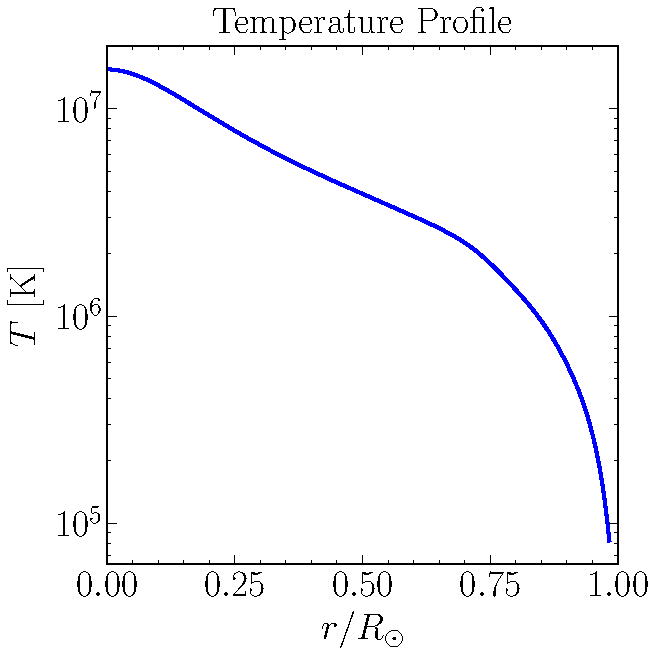
\includegraphics[width=0.3\textwidth]{Solar Model Images/T(r).pdf}
    }
    \subfigure[]{
        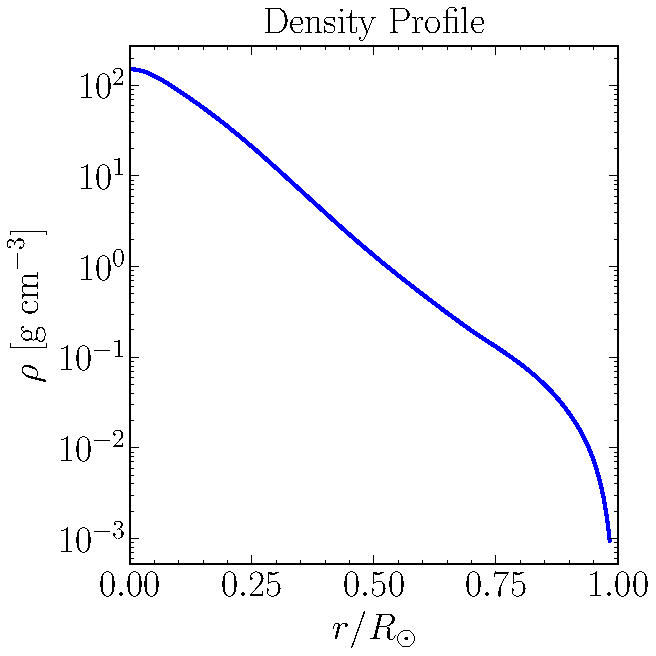
\includegraphics[width=0.3\textwidth]{Solar Model Images/rho(r).pdf}
    }
    \subfigure[]{
        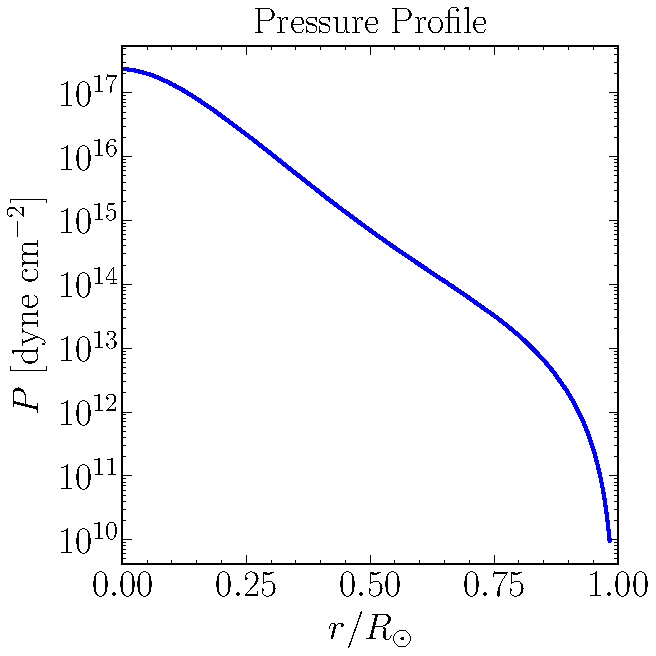
\includegraphics[width=0.3\textwidth]{Solar Model Images/P(r).pdf}
    }
    \caption{From left: temperature, density, and pressure profiles in the Sun as given by Ref.~\cite{Bahcall_2005}.}
    \label{fig:SSM_state_vars}
\end{figure}


\begin{figure}[H]
    \centering
    \subfigure[]{
        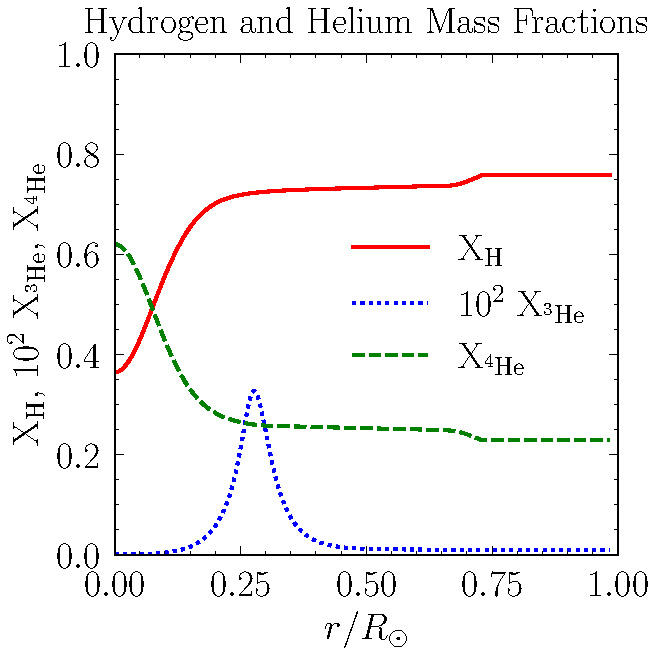
\includegraphics[width=0.45\textwidth]{Solar Model Images/X_nonmetal(r).pdf}
    }
    \subfigure[]{
        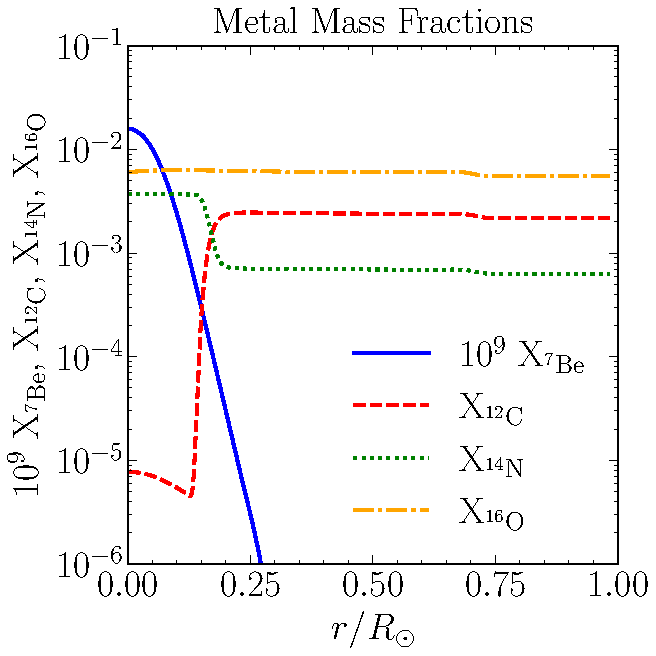
\includegraphics[width=0.45\textwidth]{Solar Model Images/X_metal(r).pdf}
    }
    \caption{Abundance profiles of Hydrogen and Helium (left) and metals (right) in the Sun as given by Ref.~\cite{Bahcall_2005}.}
    \label{fig:SSM_abundances}
\end{figure}

\begin{figure}[H]
    \centering
    \subfigure[]{
        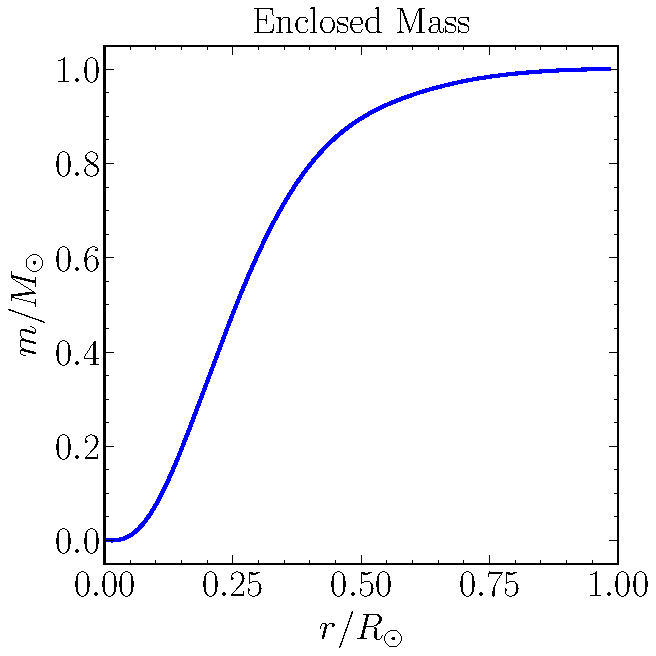
\includegraphics[width=0.45\textwidth]{Solar Model Images/m(r).pdf}
    }
    \subfigure[]{
        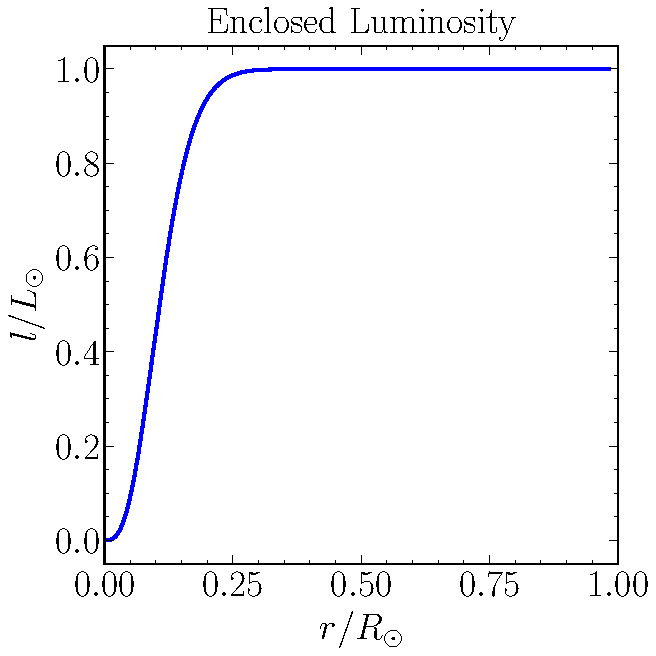
\includegraphics[width=0.45\textwidth]{Solar Model Images/l(r).pdf}
    }
    \caption{Enclosed mass (left) and luminosity (right) as a function of radius in the Sun as given by Ref.~\cite{Bahcall_2005}.\vspace{1cm}}
    \label{fig:SSM_mass_shine}
\end{figure}

\section{What heats stars?} \label{sec:heat}
\begin{flushleft} \singlespacing \vspace{-0.25cm}
    \textit{``When did you become an expert in thermonuclear astrophysics?''}\\
    \textit{``Last night."} \\
\end{flushleft} 
\begin{flushright} \vspace{-0.5cm}
    - Conversation between Maria Hill and Tony Stark, \textit{The Avengers}
\end{flushright}
\doublespacing

%
Given the luminosity of the Sun $\sim 10^{26}$ W~\cite{Kopp_2016} and its presumed age $\sim 10^9$ years~\cite{Connelly2012}, it is difficult to imagine a stellar power source. Through the physics described in Refs.~\cite{Gamow1938,Clayton1983,Rolfs1988}, we now know that \textit{``when we look up at night and view the stars, everything we see is shining because of distant nuclear fusion"}~\cite{sagan1985cosmos}. I provide only a short overview of the important nuclear reactions powering the Sun here, returning to the physics and energy generation in Section \ref{sec:shine_production}. For more details, see Appendix \ref{ap:fusion}.

\subsection{The pp Chain}
First identified in the late 1930s, the proton-proton (pp) chain is the primary mechanism via which energy is generated in Sun-like stars~\cite{Bethe1939,Phillips1999}. The process via which four Hydrogen atoms combine to form one Helium atom is split across three sub-chains, involving many individual reactions detailed in Appendix \ref{ap:nucReac}. A diagramatic representation of the pp chain is given in Figure \ref{fig:pp_pictorial}.

\begin{figure}[H]
    \centering
    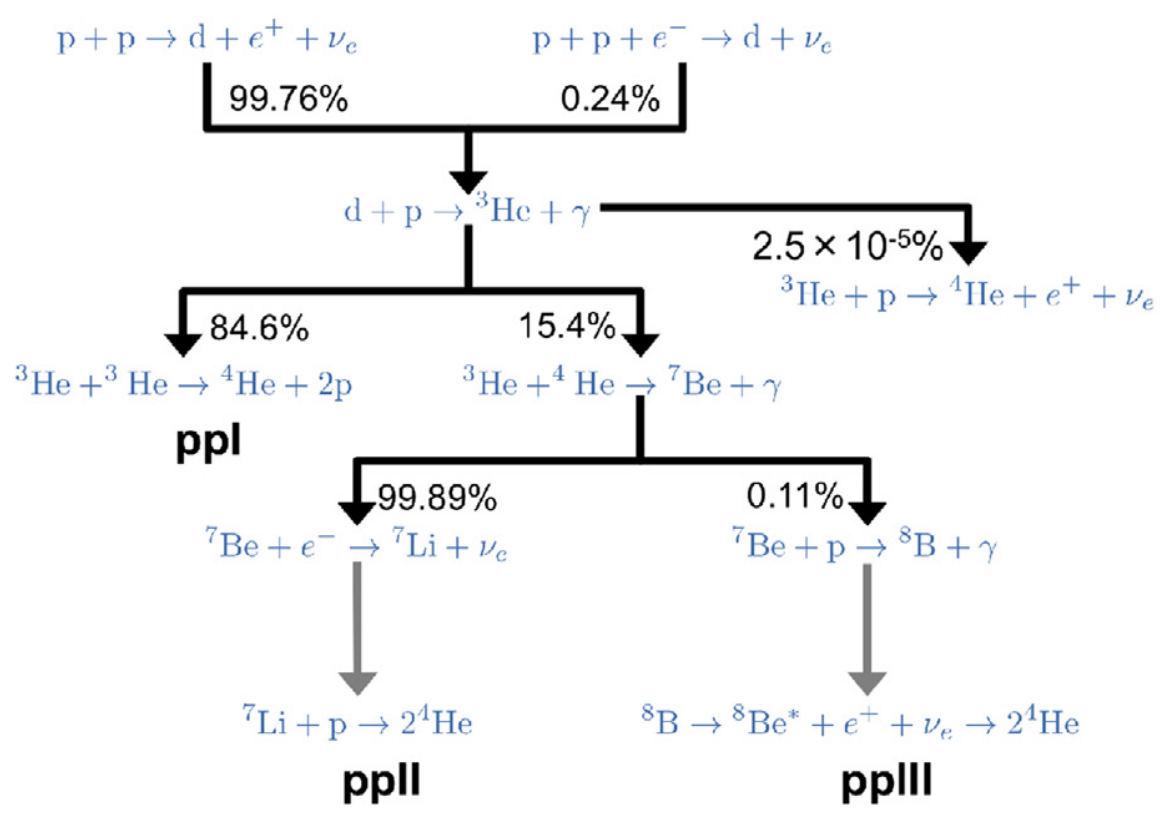
\includegraphics[width=0.5\linewidth]{Main Graphics/pp_pictorial.png}
    \caption{Schematic of the pp-chain taken from Ref.~\cite{fusionGraphics}.}
    \label{fig:pp_pictorial}
\end{figure}

\subsection{The CNO Bi-cycle}
The Carbon-Nitrogen-Oxygen (CNO) bi-cycle dominates energy production in stars more massive than the Sun~\cite{Phillips1999} due to very high temperature dependence~\cite{Prialnik}, but still plays an important role in studying the Sun. In this process, two parallel branches (see Figure \ref{fig:CNO_pictorial}) fuse Hydrogen into Helium via metal catalysts in reactions detailed in Appendix \ref{ap:nucReac}.

\begin{figure}[H]
    \centering
    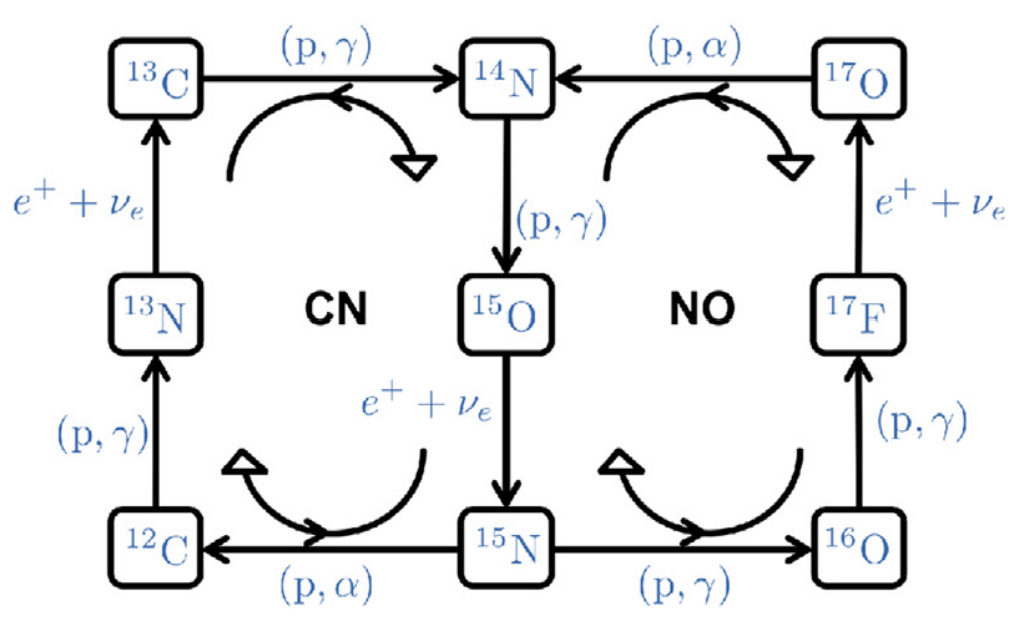
\includegraphics[width=0.5\linewidth]{Main Graphics/CNO_pictorial.png}
    \caption{Schematic of the CNO bi-cycle taken from Ref.~\cite{fusionGraphics}.}
    \label{fig:CNO_pictorial}
\end{figure}

\subsection{Keeping Stars Hot}
A star retains its heat content over the Kelvin-Helmholtz timescale even in the absence of nuclear reactions, continuing to shine. To explore this idea in more detail, reconsider the virial theorem,
%\vspace{-0.5cm}
%
\begin{equation}
    \zeta E_\mathrm{i} = E_\mathrm{g}, \tag{\ref{eq:Main_virial}}
\end{equation}
%\vspace{-1.5cm}
%
which relates internal energy to gravitational binding energy within a star via an equation of state parameter. Imagine a star which adiabatically contracts on a timescale longer than the dynamical timescale. For an ideal gas\footnote{For more on the ideal gas law, see Appendix \ref{ap:ideal_gas}.}, $\zeta = 2$, meaning that half of the energy liberated by contraction (redistribution of the gravitational binding energy) is used to heat the star (increase the internal energy of gas particles) with the remaining half radiated away as luminosity $L$:
%\vspace{-0.5cm}
\begin{equation}
    L = \deriv{E_\mathrm{i}}{t} = -\frac{1}{2} \deriv{E_\mathrm{g}}{t}
\end{equation}
%\vspace{-1.5cm}
%
As a star shines, it \textit{necessarily} stays hot by the virial theorem. For the derivation of this result, see Section \ref{sec:virialTheorem}.

\section{So, how \textit{do} stars shine?} \label{sec:shine}
\begin{flushleft} \singlespacing \vspace{-0.25cm}
    \textit{``Stars, won't you shine on me?}\\
    \textit{Won't you dance with me?"} \\
\end{flushleft} 
\begin{flushright} \vspace{-0.5cm}
    - Carly Rae Jepsen, \textit{Love Again}
\end{flushright}
\doublespacing
%
In answering the question of how stars shine, I present analytical treatments of energy generation and transport in the Sun. Using the solar model from Ref.~\cite{Bahcall_2005}, I numerically calculate and plot quantities of interest as a function of radius throughout the solar interior.

\subsection{Energy Production}\label{sec:shine_production}
The pp chain and CNO bi-cycle are responsible for energy generation in the Sun. I present the central arguments of nuclear reactions here, and offer more details in Appendix \ref{ap:rates}.

\subsubsection{Nuclear Reaction Rates}
When considering a reaction between bare atomic nuclei, one must first consider the electrostatic repulsion between the particles. A fusion reaction becomes likely to occur when the particle separation becomes comparable to the nuclear radius ($r_0 \sim 10^{-15}$ m). For a projectile $a$ and a target nucleus $b$, the height of the Coulomb barrier is of order $ E_\mathrm{C} \sim Z_a Z_b$ MeV, where $Z_i$ are the atomic numbers of the reactants involved. For a Maxwellian distribution of particles, this corresponds to a temperature in excess of $10^{10}$ K. This is far above the typical range of temperatures in stellar interiors and gives a probability of $\sim 10^{-481}$ for the fusion reaction between two protons. From classical arguments alone, it would seem that nuclear fusion is an impossibility as a power source for the Sun.

The application of quantum mechanical tunneling in Ref.~\cite{Gamow1938} demonstrated that the Coulomb barrier need not be breached via ``brute force", with the probability of a reaction scaling with center-of-mass energy $E$ as

\begin{equation}
    p(\text{reaction}) \approx \exp\left[-\bigparenthesis{\frac{E_\mathrm{G}}{E}}^{1/2}\right]
\end{equation}
%
where $E_\mathrm{G}$ is the Gamow energy. For the fusion of two protons in the Sun at $r/R_\odot \sim 0.1$, the temperature corresponds to $E \sim 1$ keV and $E_\mathrm{G} \approx 500$ keV~\cite{Phillips1999}, giving a probability of $\sim 10^{-10}$. This still seemingly low probability for fusion is compensated by the $\sim 10^{56}$ protons within the inner 10\% of the Sun.

To calculate nuclear reaction rates, two main ingredients are needed. The number densities $n_i$ of the reactants must play a role, as well the probability that the reactions occur. The reaction rate per volume per second is thus given by

\begin{equation}
    \Gamma_{ab} = \frac{n_a n_b}{1 + \delta_{ab}} \left<\sigma v\right> \label{eq:main_reactionrate}
\end{equation}
%
where the Kronecker delta is included in the denominator to correct for double-counting. The final factor in Equation \ref{eq:main_reactionrate} contains the relevant microphysics encoding the reaction probability per pair of reactants, and is a weighted average in energy of the product of the fusion cross section $\sigma(E)$ and velocity $v(E)$ distribution of particles $f(E)$:

\begin{equation}
    \left< \sigma v \right> = \int_0^\infty dE v(E)f(E)\sigma(E)\label{eq:main_sigmav}
\end{equation} 


The cross section factor in Equation \ref{eq:main_sigmav} is dependent on the reaction of interest, and often contains nuclear resonances complicating the evaluation of the energy integral. The consideration of nuclear resonances is complex\footnote{For a discussion of resonant contributions, see Chapters 4.4 -- 4.7 in Ref~\cite{Cox_Giuli_vol1}.} and not important within the stars of interest in this report, so I proceed by calculating non-resonant contributions. Energy-dependent behavior in the cross section is encapsualted via the experimentally determined ``astrophysical S factor" defined by

\begin{equation}
    \sigma(E) = \frac{S}{E} \exp\bigparenthesis{-\sqrt{\frac{E_\mathrm{G}}{E}}}.
\end{equation}
%
For a non-relativistic Maxwellian distribution of particles, we obtain

\begin{equation}
     \left< \sigma v \right> = \frac{2\sqrt{2}}{\sqrt{m_r\pi}} \frac{1}{(k_B T)^{3/2}} \int_0^\infty dE S(E) \exp\bigparenthesis{-\frac{E}{k_B T} -\sqrt{\frac{E_\mathrm{G}}{E}}} \label{eq:Maxwell_sigmav}
\end{equation}
%
where $m_r$ is the reduced mass of the reactants. The most interesting part of the integrand in Equation \ref{eq:Maxwell_sigmav} is the exponential term, wherein two competing physical phenomena produce a compromise; the exponential tail of the Maxwell-Boltzmann distribution is compensated by the increasing probabilty for quantum tunneling. This produces a characteristic shape known as a Gamow peak (see Figure \ref{fig:Gamow}), outside of which there is vanishing contribution to the integral. 

\begin{figure}
    \centering
    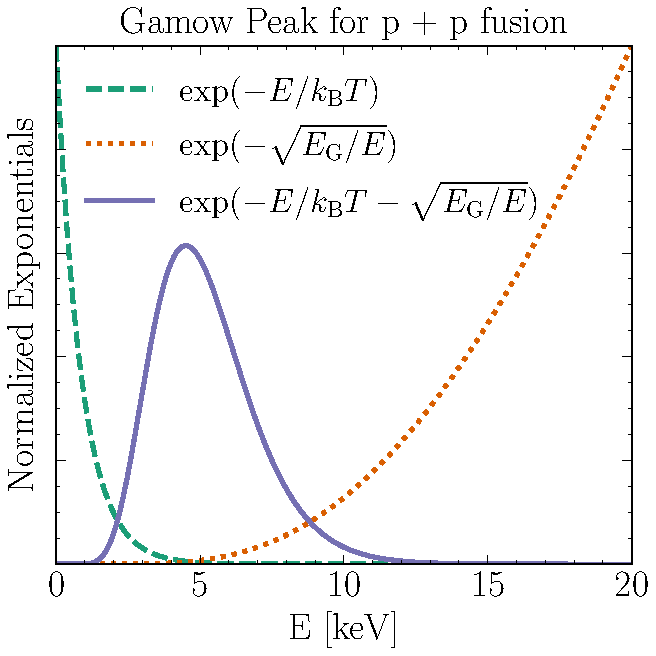
\includegraphics[width=0.5\linewidth]{Main Graphics/Gamow.pdf}
    \caption{Demonstration of how the exponential tail of the Maxwell-Boltzmann distribution and the tunneling probability combine to form a Gamow peak for the fusion of two protons. The exponential functions in this plot are arbitrarily normalized for visual clarity.}
    \label{fig:Gamow}
\end{figure}

At astrophysical energies, $S(E)$ is typically a very slowly varying function in the absence of known resonances. It is typical to write an effective S factor $S_\mathrm{eff}$ as Maclaurin series for which coefficients are determined from theory and measurements. Additionally, one can include a simple numerical approximation of the effect of electron screening on the reaction rates given by a screening parameter $f_0$~\cite{Saltpeter1954}. These approaches are reasonable due to the ``tame" nature of the interiors of Sun-like stars. The energy range of Gamow peaks for the Hydrogen-fusing reactions of interest happen to fall outside of sharp nuclear resonances and regimes of strong electron screening, and the typical temperatures and densities do not significantly\footnote{See Appendix \ref{ap:departures} for departures from non-relativisitic, classical mechanics in the Sun.} stray far from non-degenerate and non-relativistic conditions~\cite{Clayton1983,Cox_Giuli_vol1,Christensen_Dalsgaard_2021}. For the purposes of addressing how stars shine, I comfortably use the approximation for the $\left<\sigma v\right>$ given in Ref.~\cite{bahcall1989neutrino} as


\begin{equation}
    \left<\sigma v \right> = 1.3005 \times 10^{-15} \left[\frac{Z_a Z_b}{A T_6^2}\right]^{1/3} f_0 S_\mathrm{eff} \exp{(-\tau)} \text{ cm}^{3} \text{ s}^{-1} \label{eq:sigmav_approximation}
\end{equation}
%
where $\tau$ is approximately the argument of the exponent in Equation \ref{eq:Maxwell_sigmav} having the form

\begin{equation}
    \tau = 3 \left[\pi \bigparenthesis{\frac{m}{2k_B T}}^{1/2} \frac{Z_a Z_b e^2}{\hbar^2} \right]^{2/3} \approx 42.487 (Z_a^2 Z_b^2 A T_6^{-1})^{1/3}
\end{equation}
%
where $A$ is the reduced atomic mass of the reactants, and $T_6 = T/10^6$~\cite{KWW_book,bahcall1989neutrino}. Rates for selected reactions of the pp chain and CNO bi-cycle in the Sun are shown in Figures \ref{fig:pp_Reactions} and \ref{fig:cno_Reactions}. For more details regarding the quantities involved, see Appendix \ref{ap:SunRates}.

\begin{figure}
    \centering
    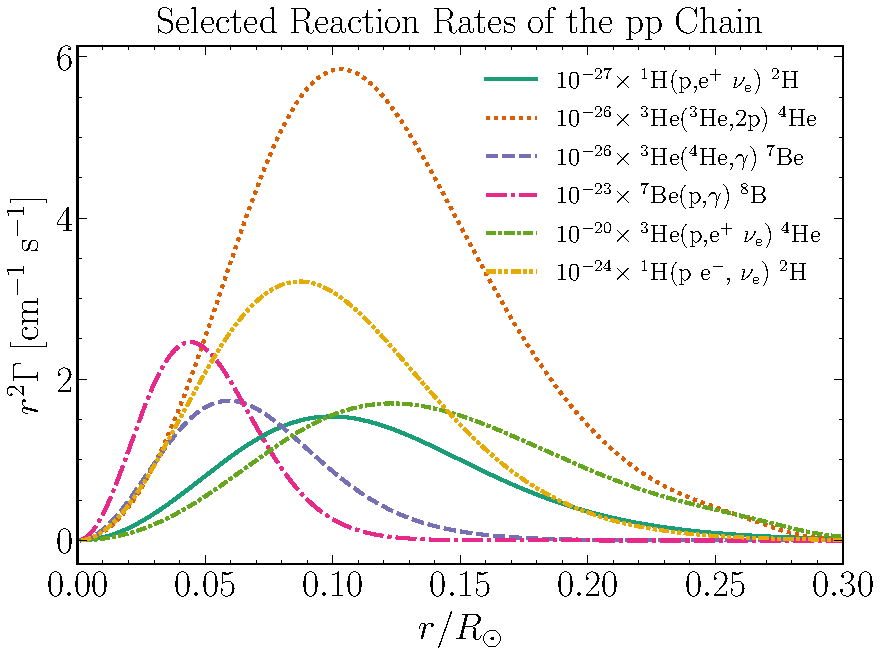
\includegraphics[width=0.75\linewidth]{Main Graphics/pp_rates.pdf}
    \caption{Reaction rates for selected reactions of the pp chain in the Sun computed using Equation \ref{eq:main_reactionrate} and \ref{eq:sigmav_approximation}. Reactions are appropriately scaled for visual comparison, and are labeled using the following notation: Target(projectiles,by-products)Product}
    \label{fig:pp_Reactions}
\end{figure}

\begin{figure}
    \centering
    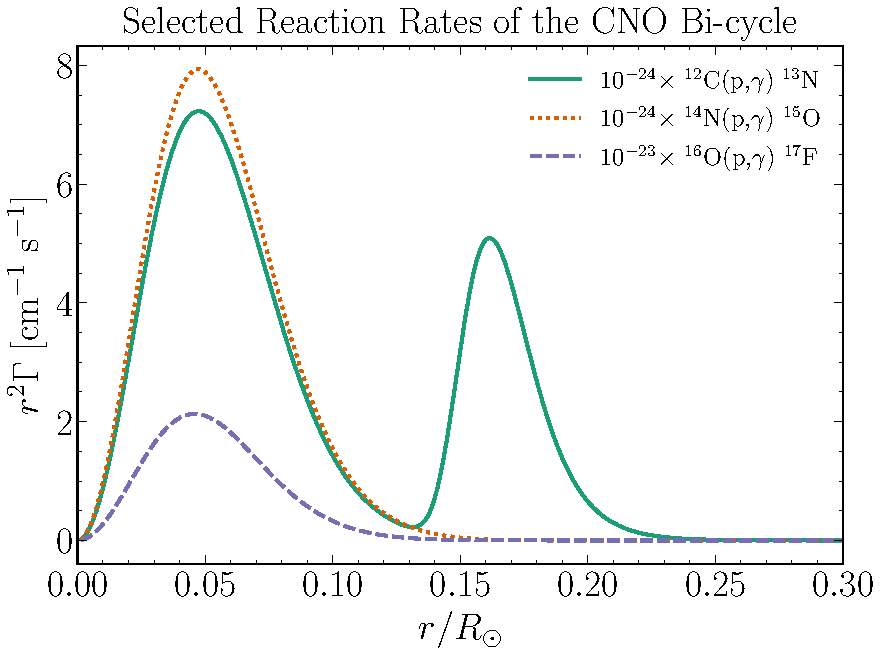
\includegraphics[width=0.75\linewidth]{Main Graphics/cno_rates.pdf}
    \caption{Same as Figure \ref{fig:pp_Reactions} but for selected reactions of the CNO bi-cycle.}
    \label{fig:cno_Reactions}
\end{figure}

Returning to the point that stars are powered by \textit{thermo}nuclear reactions, fusion reaction rates can be well-described by their temperature dependence following the procedure in Chapter 18.3 of Ref.~\cite{KWW_book} . The temperature dependence of $S_\mathrm{eff}$ and $f_0$ are very weak, while $\tau \sim T^{-1/3}$. The quantity $\left<\sigma v \right>$ accordingly scales as $\sim T^{-2/3} \exp{(-\tau)}$. One can then approximate the reaction rate as a power law of the form

\begin{equation}
    \Gamma \sim \left<\sigma v \right> = \left<\sigma v \right>_0 \bigparenthesis{\frac{T}{T_0}}^\nu,\text{ } \nu = \pderiv{\ln \left<\sigma v \right>}{\ln T} \label{eq:powerLaw}
\end{equation}
%
where $\left<\sigma v \right>_0$ is a normalization factor and $T_0$ is some reference temperature. Taking the natural log of Equation \ref{eq:powerLaw} and differentiating with respect to $\ln T$,

\begin{align}
    \ln  \left<\sigma v \right> &= \text{constant} - \frac{2}{3}\ln T - \tau \\
    \pderiv{\ln \left<\sigma v \right>}{\ln T} &= -\frac{2}{3} - \pderiv{\tau}{\ln T} = -\frac{2}{3} - \tau\pderiv{\ln\tau}{\ln T} = \frac{\tau}{3} - \frac{2}{3}.
\end{align}

For the lightest reaction at the solar core between two protons, $\tau \approx 13$, giving $\nu_\mathrm{11} \sim 4$. For reactions involving heavier constituents such as the fusion of $^{7}$Be and a proton, $\tau \approx 41$, giving $\nu_\mathrm{17} \sim 13$. Reaction rates are more accurately modeled using somewhat higher values of $\nu$ in practice due to dependencies on composition or density.

\subsubsection{Generation of Luminosity}
Having described the rates of nuclear reactions, I now move on to describing reaction energetics. One can consider energy generated per reaction, $Q$, from first principles via the liberation of nuclear binding energy from fusing four protons into a Helium nucleus:


\begin{equation}
    Q = (4m_\mathrm{p} - m_{^{4}\mathrm{He}})c^2
\end{equation}


The quantity $m_{^4\mathrm{He}}$ is the mass of the Helium \textit{nucleus}, but since $m_\mathrm{p}/m_\mathrm{e} \approx 1800$, it is reasonable to evaluate the energy per reaction using the atomic mass. For the general transmutation of $4\text{p} \rightarrow\text{ } ^4\text{He}$, $Q \approx 27.4$ MeV is produced and injected into the surroundings. From $Q$ we can define an energy content $\varepsilon$ of this transmutation as


\begin{equation}
    \varepsilon = \frac{Q}{4 m_\mathrm{p}} = 6.56 \times 10^{4} \text{ erg/g},
\end{equation}
%
which when multiplied by 0.1 solar masses and divided by the solar luminosity, approximately reproduces the nuclear timescale:

\begin{equation}
    \frac{0.1 \varepsilon M_\odot}{L_\odot} \approx 10^{10} \text{ yr} \approx \tau_\mathrm{n}
\end{equation}
%
This should not be surprising, since $\varepsilon/c^2 \approx 7.3\times 10^{-3} \sim 10^{-2}$, the ``efficiency" of Hydrogen fusion that went into the expression for the nuclear timescale.

One might crudely imagine obtaining a nuclear energy generation rate for use in Equation \ref{eq:Main_energy} via $\epsilon_\mathrm{n} = Q\Gamma_{4\mathrm{p} \rightarrow \text{} ^4\text{He}}$, which while demonstrative of the general procedure, is not so simple. The pp chain and CNO cycle are made of many reactions, each with different rates and energetics. Careful treatments of the \textit{energy} generation rates involve counting the fractions of $^4$He nuclei produced by each chain/cycle, identifying rate-limiting reactions, considering how chains may terminate, abundances of various isotopes, and energy losses from reactions involving the production of neutrinos. Analytical expressions differ between approaches but generally produce similar behaviors, so I adopt the easily usable effective energy generation rates from Ref.~\cite{KWW_book} given by

\begin{align}
    \epsilon_\mathrm{pp} &= \frac{2.4 \times 10^{4} \rho X_\mathrm{H}^2}{T_9^{2/3}}\exp\left(\frac{-3.380}{T_9^{1/3}}\right) \text{ erg} \text{ g}^{-1} \text{ s}^{-1} \\
    \epsilon_\mathrm{CNO} &= \frac{4.4\times10^{25} \rho X_\mathrm{H}^2 Z}{T_9^{2/3}} \exp\left(\frac{-15.228}{T_9^{1/3}}\right) \text{ erg} \text{ g}^{-1} \text{ s}^{-1}
\end{align}
%
where $X_\mathrm{H}$ is the mass fraction of Hydrogen, $T_9 = T/10^9$, $\rho$ is the usual mass density in units of g cm$^{-3}$, and $Z$ is the mass fraction of metals. In Sun-like stars, the pp chain dominates over the CNO bi-cycle (see Figure \ref{fig:energy_gen}) but this relation flips for more massive stars.  For detailed and technical discussions on the procedure of calculating energy generation rates, see Chapter 17.17 of Ref.~\cite{Cox_Giuli_vol1}, Chapters 5.1-5.4 of Ref.~\cite{Clayton1983}, and Chapter 6.1.3 of Ref.~\cite{Rolfs1988}.

\begin{figure}
    \centering
    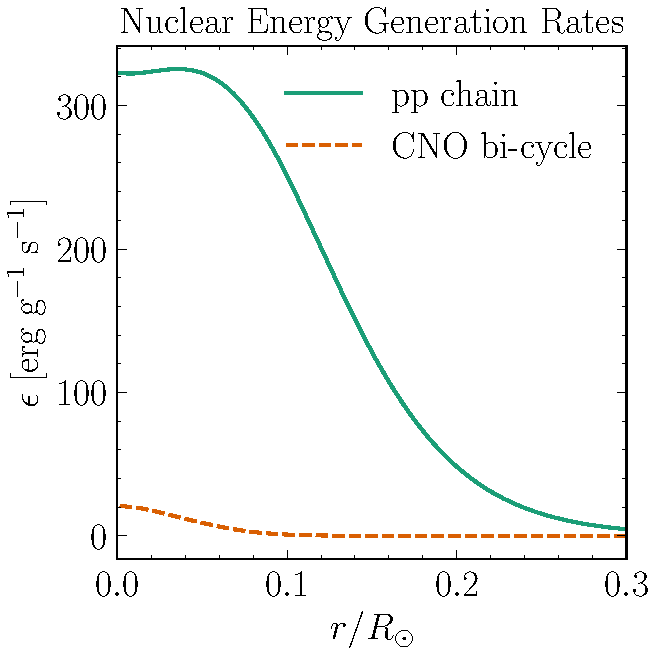
\includegraphics[width=0.5\linewidth]{Solar Model Images/energy_gen.pdf}
    \caption{Effective energy generation rates for the pp chain and the CNO bi-cycle.}
    \label{fig:energy_gen}
\end{figure}

In addition to the neutrinos produced directly from nuclear reactions, various particle physics processes within stellar interiors contribute to $\epsilon_\nu$ in Equation \ref{eq:Main_energy} to varying degrees. If $\epsilon_\nu$ is interpreted to be the specific energy rate at which neutrinos are produced~\cite{HK_book}, then the minus sign in Equation \ref{eq:Main_energy} indicates that the production of neutrinos is a power drain on the star. How can this be? The typical neutrino capture cross section scales like

\begin{equation}
    \sigma_\nu \sim 10^{-44} \text{ cm}^2 \bigparenthesis{\frac{E_\nu}{10 \text{ MeV}}}^{-2}, 
\end{equation}
%
where $E_\nu$ is the neutrino energy~\cite{KWW_book}. The mean free path of neutrinos can be calculated using $\lambda = m_\mathrm{p}/\rho\sigma_\nu$ to obtain

\begin{equation}
    \lambda \sim 10^{19} \text{ cm} \bigparenthesis{\frac{E_\nu}{10 \text{ MeV}}}^{-2} \bigparenthesis{\frac{\rho}{100 \text{ g cm}^{-3} }}^{-1},
\end{equation}
%
which is much larger than the size of the Sun ($R_\odot \sim 7 \times 10^{10}$ m). As such, neutrinos do not deposit their energy within stellar interiors. While not significant in the Sun, discussions on neutrino energy losses can be found in Chapter 18.7 of Ref.~\cite{KWW_book}, Chapter 6.8 of Ref.~\cite{HK_book}, and references therein, with approximate expressions for $\epsilon_\nu$ given in Chapter 17.20 of Ref.~\cite{Cox_Giuli_vol1}.

\subsection{Energy Transport}
The preceding subsection covered the production of energy within stars, which by the condition of thermodynamic equilibrium, powers the blackbody photon fields within stellar interiors. In essence, the ``shine" has been produced, and what remains is to follow it as it flows out of the star. I now turn my attention to the transport of energy through Sun-like stars, focusing on the physical mechanisms.

Energy is transported via radiation and convection in the main sequence stars of interest. The dominant energy transport mechanism at a particular radial shell defines the ``zone" the shell belongs to. The Sun's core is characterized by radiative transport, while the envelope is convective (see Figure \ref{fig:transportImage}). This arrangement is reversed for stars of higher mass, with less massive stars being entirely convective~\cite{KWW_book}. 

\begin{figure}[H]
    \centering
    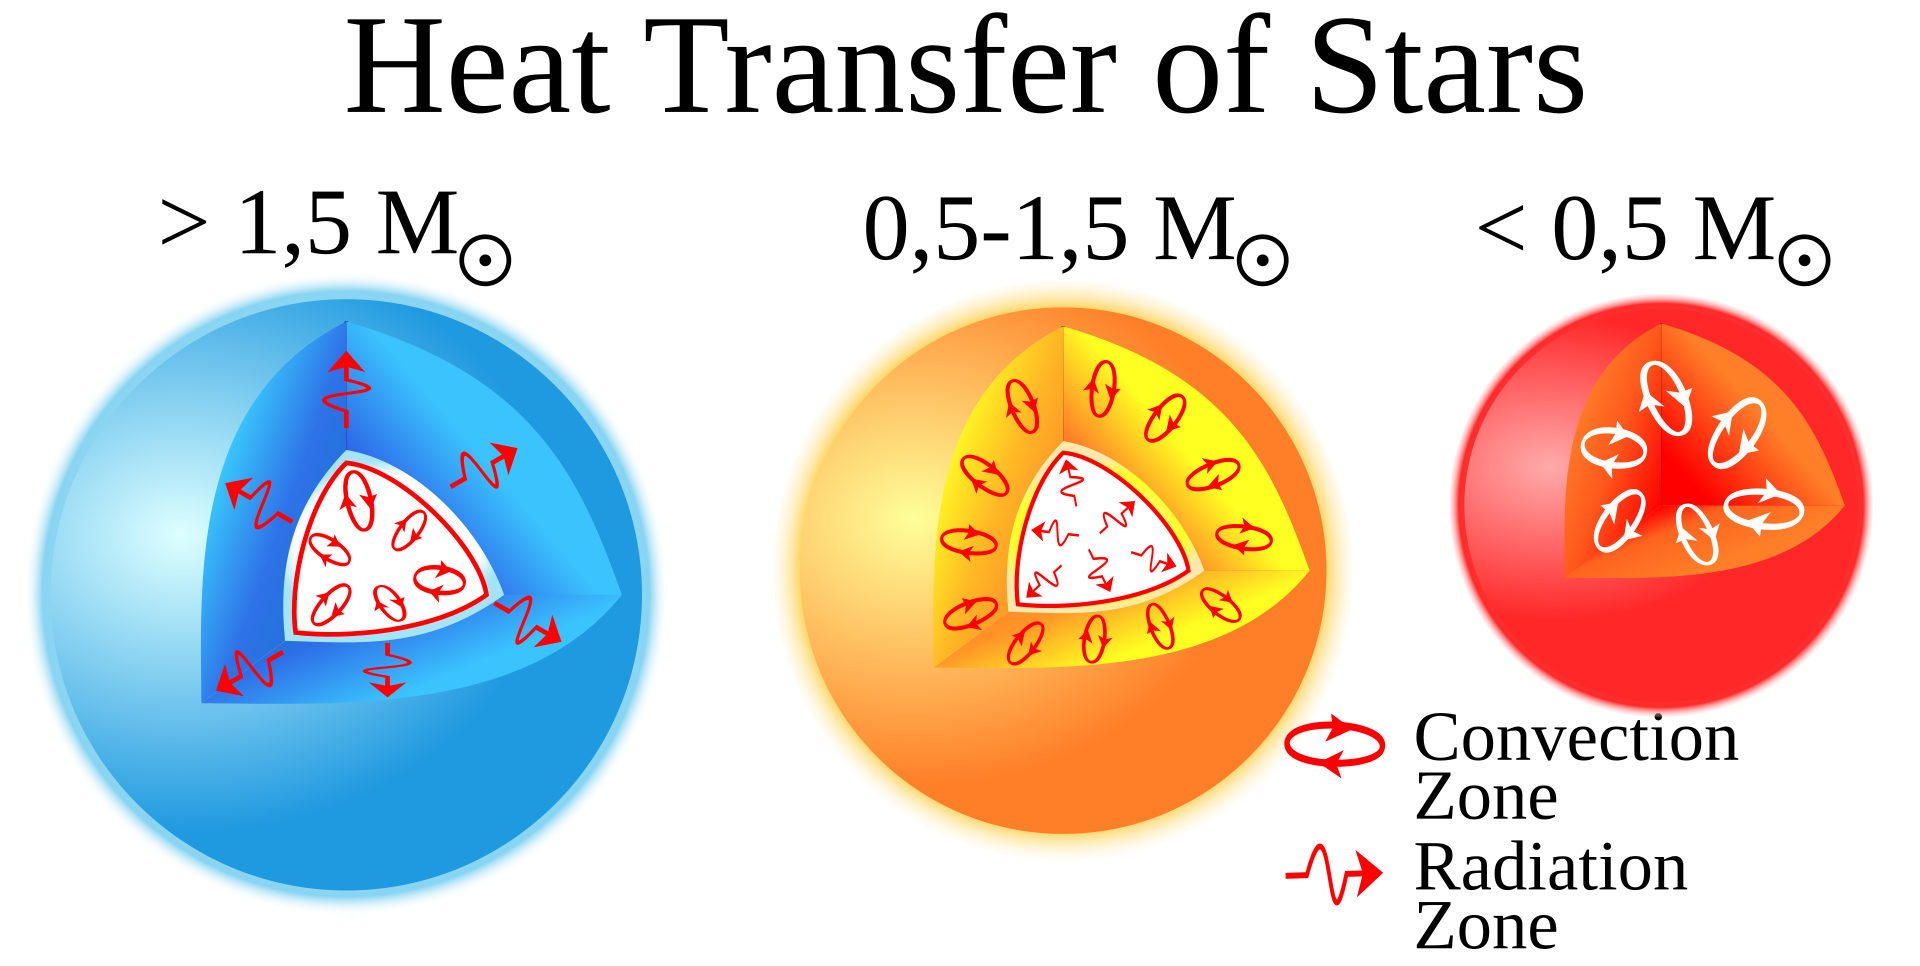
\includegraphics[width=0.5\linewidth]{Main Graphics/Heat_transfer.png}
    \caption{Energy transport mechanisms within stars, highlighting radiative and convective zones~\cite{transportImage}.}
    \label{fig:transportImage}
\end{figure}

The discussion regarding energy transport centers around the equation of thermal structure

\begin{equation}
    \pderiv{T}{r} = \frac{Gm\rho}{r^2}\frac{T}{P} \nabla,\tag{\ref{eq:Main_thermal}}
\end{equation}
%
focusing on the temperature gradient $\nabla = \pderiv{\ln T}{\ln P}$. The temperature gradient in Equation \ref{eq:Main_thermal} is the \textit{actual} logarithmic slope of temperature versus pressure, and is a general expression evaluated within the stellar interior agnostic to the mechanism via which energy is transported. 

When energy transport is entirely from the diffusion of photons, the temperature gradient is given by $\nabla = \nabla_\mathrm{rad}$ for radiative transport. Such portions of stars are said to be under radiative equilibrium, wherein the rate of emission of electromagnetic energy is compensated by the rate of absorption~\cite{Cox_Giuli_vol1}. The role of opacity is thus essential in describing radiative transport. 

When energy is transported via adiabatically rising and falling parcels of gas, the temperature gradient is $\nabla = \nabla_\mathrm{ad}$ for convective transport. Here, $\nabla_\mathrm{ad}$ characterizes the gas parcels themselves. In this scheme, a parcel of gas may experience a temperature fluctuation, causing it to expand, decrease in density, and move radially outward without transferring heat to the surroundings. After the parcel has risen some characteristic length, it dissolved into its new surroundings, transporting heat in the process. Note that there is a net \textit{energy} flux, but no net \textit{mass} flux.

In the following subsections I present the main results of analytical treatments of radiative and convective transport and the important physics therein, showcasing important conclusions within the Sun using numerical computations. Derivations are included in Appendices \ref{ap:rad_transport} and \ref{ap:convection}.

\subsubsection{The Radiative Core}
Energy produced by nuclear reactions in the cores of stars is dumped into the stellar material at thermodynamic equilibrium, giving rise to blackbody radiation fields. The blackbody photons then diffuse outwards and interact with the layers of the star. Following the derivation in Appendix \ref{ap:rad_transport}, the radiative temperature gradient is given by

\begin{equation}
    \nabla_\mathrm{rad} = \bigparenthesis{\pderiv{\ln T}{\ln P}}_\mathrm{rad} = \frac{P}{T} \frac{\partial T/ \partial r}{\partial P/\partial r} = \frac{3\kappa l P}{16\pi \sigma_\mathrm{SB} c G m T^4} \label{eq:nabla_rad}
\end{equation}
%
with opacity $\kappa$ and luminosity $l$. The various expressions in Equation \ref{eq:nabla_rad} are worth discussion. The first and second equalities hold only if energy transport is solely described by radiative mechanisms. In other words, attributing a calculation of $\frac{P}{T} \frac{\partial T/ \partial r}{\partial P/\partial r}$ over the entire star to represent radiative transport as the \textit{actual} energy transport is physically meaningful only in the absence of other mechanisms. Likewise, the final equality only applies if the \textit{actual} energy transport in some region of the stellar interior is dominated by radiative transport.

The final ingredient precluding the computation of $\nabla_\mathrm{rad}$ is the opacity $\kappa$. In general, the opacity is a very involved function of density, temperature, composition, photon frequency, and ionization states that is frequently presented in tabular form. To alleviate some of this complexity, one can define a monochromatic opacity known as the Rosseland mean opacity $\bar{\kappa}$ for which there exist simple approximate forms for the canonical absorption mechanisms~\cite{EracleousPSU}. See  Appendix \ref{ap:opacity} for approximate formulae for sources of opacity.

\subsubsection{The Convective Envelope}
To determine which energy transport mechanism is at play at different layers of a star, one appraises a stability condition that arises from physical arguments involving several temperature gradients. For a displaced parcel of gas to continue rising, the density inside the parcel must drop faster than the density of the parcel's surroundings~\cite{KWW_book}. Consequently,

\begin{equation}
    \bigparenthesis{\pderiv{\rho}{r}}_\mathrm{parcel} > \bigparenthesis{\pderiv{\rho}{r}}_\mathrm{star} \label{eq:main_convec_stab}
\end{equation}
%
for a region to be \textit{stable} against convective motion\footnote{Note that $\partial\rho/\partial r < 0$, which may alleviate some confusion regarding the direction of the inequality in Equation \ref{eq:main_convec_stab}.}. For a region of homogeneous chemical composition, the Schwarzchild criterion for dynamical stability\footnote{See Appendix \ref{ap:convec_stability} for a derivation.} states that if

\begin{equation}
    \nabla_\mathrm{rad} < \nabla_\mathrm{ad}, \label{eq:convectionStability}
\end{equation}
%
convective motion does not occur. This condition is appraised while evaluating the equation of thermal structure in stellar model codes to most accurately describe energy transport.

When considering the stability condition in Equation \ref{eq:convectionStability}, convection will start to kick in when the radiative temperature gradient gets too high. How high? Assuming the gas parcels are ideal and undergo adiabatic changes\footnote{See Appendix \ref{ap:nabla_ad_ideal} for details regarding Equation \ref{eq:0.4}.},

\begin{equation}
    \nabla_\mathrm{ad} = \frac{P\delta}{T\rho c_P} = \frac{2}{5}. \label{eq:0.4}
\end{equation}

Once $\nabla_\mathrm{rad} > \frac{2}{5}$ at some radial shell in the star, convection will begin to take over as the dominant form of energy transport. Via the first equality in Equation \ref{eq:nabla_rad}, one can use the temperature and density profiles from a stellar model and calculate the radiative temperature gradient throughout the star. Then, the location of the base of the convective envelope can be identified via the Schwarzchild criterion. The result of this computation for the Sun is in Figure \ref{fig:nabla_rad}, suggesting that convection sets in at $r/R_\odot \approx 0.74$ and extends towards the Solar surface. Seismic observations of the Sun suggest a precise value closer to $r/R_\odot \approx 0.71$~\cite{convectiveZone}. Figure \ref{fig:texas} is an image of the convective cells right below the Sun's photosphere.

\begin{figure}
    \centering
    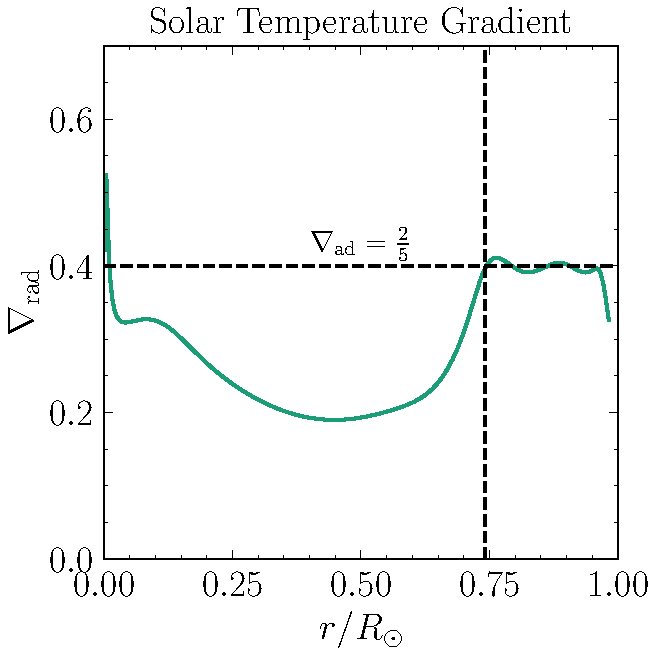
\includegraphics[width=0.5\linewidth]{Solar Model Images/nabla_rad.pdf}
    \caption{Evaluation of the radiative temperature gradient within the Sun. From the Schwarzschild criterion in Equation \ref{eq:convectionStability}, a simple estimate of the base of the convective zone is $r/R_\odot \approx 0.74$.}
    \label{fig:nabla_rad}
\end{figure}

\begin{figure}
    \centering
    \includegraphics[width=0.5\linewidth]{Main Graphics/granule.jpg}
    \caption{Photograph of the convection cells in the  Sun's photosphere~\cite{NSF_2020}, where the scale of the typical cell is comparable to the size of Texas $\sim 7\times10^{11}$ m$^2$.}
    \label{fig:texas}
\end{figure}

\subsubsection{The Photosphere}
As state variables drop with radius, $\nabla_\mathrm{rad}$ relaxes and energy transport is once again dictated by the diffusion of photons near the Sun's surface. This thin (depth $\sim 500$ km), cool ($T \sim 5000$ K), and only easily visible region of the solar interior is known as the photosphere. The density of particles drastically drops off in the photosphere and above (optical depth $\tau \approx 2/3$~\cite{BoB}), allowing photons to escape from the star and propagate into space. At last, the Sun shines, bathing the universe with $3.828 \times 10^{33}$ erg s$^{-1}$ of electromagnetic energy~\cite{Kopp_2016}.

One can determine the effective temperature of stars using measurements of luminosity. Here, ``effective temperature" corresponds to the blackbody temperature of the stellar photosphere. Via the Stefan-Boltzmann law,

\begin{equation}
    L = 4\pi R^2 \sigma_\mathrm{SB} T_\mathrm{eff}^4,
\end{equation}
%
and $R_\odot = 6.957 \times 10^{10}$ cm~\cite{Haberreiter_2008}, one finds that $T_\mathrm{eff} \approx 5770$ K for the Sun. 

\section{Why study stars?} \label{sec:why}
\begin{flushleft} \singlespacing \vspace{-0.25cm}
    \textit{``Don't you see the starlight, starlight?}\\
    \textit{Don't you dream impossible things?"} \\
\end{flushleft} 
\begin{flushright} \vspace{-0.5cm}
    - Taylor Swift, \textit{Starlight}
\end{flushright}
\doublespacing
%
In answering how stars shine, I have explored many rich topics in physics in this report. While I am an astrophysicist at heart, I hope that my ``terraphysicist" colleagues can still agree that stars are fascinating subjects to study. In this section, I provide a short overview of observations and experiments relevant to the preceding theoretical discussions, as well as uncertainties and active areas of research regarding both microphysics and stellar structure. Involved discussions of these topics is not feasable in this report, and so I include several potentially illuminating references throughout this section.

\subsection{Uncertainties in Stellar Structure}
In contrast to the stipulations made in Section \ref{sec:structure}, the modeling of \textit{real} stars is a serious and laborious undertaking. While the general structure of main sequence stars is well understood, there remain potentially significant physics that are either ignored or heavily simplified due to computational complexity. For example, diffusion of atomic species and gravitational settling were not included in early ``standard" solar models (SSMs), and rotation or deviations from spherical symmetry are not universally considered~\cite{Christensen_Dalsgaard_2021}.

\subsubsection{Beyond the Standard Solar Model}
Limitations from SSMs in describing the real physical systems come from the assumptions made when building such models. For instance, while spherically symmetry is a good approximation globally, it may not be appropriate for local processes. Convection, (differential) rotation, diffusion, angular momentum, and magnetic fields are inherently multi-dimensional phenomena, which cannot be carefully described using only the radial coordinate. In addition, the accurate treatment of stellar opacity remains complicated. For literature resources on these active problems, see Refs.~\cite{Vinyoles_2017,Gough_2015,Turck2011} and references therein.

\subsubsection{The Solar Abundance Problem}
The abundances (mass fractions) of metals are important quantities necessary for accurately calculating the radiative opacities within stellar interiors, affecting the general problem of stellar modeling since the differential equations of stellar structure are coupled. Even sophisticated solar models have around 2.5\% uncertainties on opacity calculations~\cite{Villante2019AnUD}. Predictions of abundances from solar model codes are at odds with spectroscopic evidence of the photosphere, and remains an unsolved problem~\cite{Bergemann_2014}. Even so, solar models which incorporate the observed abundances cannot reproduce behavior consistent with observations of solar seismic activity~\cite{Villante2019AnUD}. 


\subsubsection{Helioseismology}
In considering the restoration of hydrostatic equilibrium described in Section \ref{sec:equilibria}, dynamically stable stars are in effect oscillating on timescales on the order of the dynamical timescale. The discovery of small oscillatory motions ($ \sim 3 \text{ cm} \text{ s}^{-1}$) of the photosphere on short ($\sim$ 1--10 minute) timescales birthed the field of helioseismology which serves as a useful constraint on solar models and microphysics~\cite{Phillips1999}. 

The observation of oscillatory modes in the Sun can extract information about variable profiles within the solar interior in a process known as inversion~\cite{Buldgen_2019}. Helioseismology provides external constraints on convection~\cite{Hanasoge_2016}, abundances~\cite{Basu_2008}, the speed of sound~\cite{CD1985Nature}, and other quantities of interest within the Sun. A gentle introduction to the theory of stellar oscillations can be found in Chapter 7 of Ref.~\cite{Phillips1999}, with more advanced treatments in Refs.~\cite{HK_book,PulsatingCox,Cox_Giuli_vol2}. Reviews of helioseismology can be found in Refs.~\cite{Pall2015,CDHelioseismology}.



\subsection{Laboratories for Nuclear and Particle Physics}
The typical temperatures and densities of stellar interiors creates conditions wherein broad phenomena in subatomic physics interplay with each other. For example, the equation of state underpins the dynamics of stars, and even stars like the Sun offer a setting to test relativistic and degenerate effects (see Appendix \ref{ap:departures}). Stellar energy generation offers a direct window to studying the kinematics of fusion, which involves a plethora of connections between the strong, weak, and electromagnetic interactions (see Appendix \ref{ap:fusion}).

As such, stars of all forms serve as enticing playgrounds for theorists, observers, and experimentalists in nuclear and astroparticle physics. Among the rich sectors of physics probed by the studies of stars at large, the Sun alone enables fascinating contemporary work in understanding gamma-ray emission~\cite{OSUGamma2018,Puzzoni2023}, neutrino physics~\cite{SK2024,Borexino2017}, dark matter~\cite{Ranjan2023,IceCube2016}, and a myriad of other topics. In this subsection, I discuss the role of the Sun in exciting areas of nuclear and astroparticle physics.

\subsubsection{Neutrino Mixing Parameters}
Neutrinos produced from nuclear reaction in the Sun are effective probes of the physics and conditions near the center of the Sun, and are intimately connected with the historical development of SSMs~\cite{bahcall1989neutrino}. Since the Homestake experiment~\cite{DAVIS199413} and the discovery of solar neutrino oscillations in resolving the solar neutrino problem~\cite{SNoscillations}, much attention has been given to studying the physics of neutrinos themselves~\cite{Xu_2023}. 

Neutrinos are peculiar particles in that they only interact via the weak interaction, are very light ($m_\nu c^2 \lesssim 1$ eV~\cite{Burros1987}), and oscillate between three flavor states as they propagate through space. The mixing of neutrino flavors is physics beyond the Standard Model, and much work has been done to determine neutrino mixing parameters~\cite{Esteban2018,deSalas2020}. While tension remains in the values of mixing parameters between solar and reactor neutrino experiments~\cite{SK2024}, the incredible precision of current and planned neutrino experiments~\cite{Capozzi2019} allow for neutrinos to serve as probe of state variables within the Sun~\cite{LaberSmith:2024}.

\subsubsection{Astrophysical S-Factors}
Calculating nuclear reaction rates involves understanding the nuclear physics and cross sections of various fusion reactions, neatly baked into the astrophysical S factor. The cross section $\sigma(E)$ for various reactions can only be measured at energies around 100-200 keV, below which cross sections are too small to measure~\cite{Cox_Giuli_vol1,Acharya2024}. Meanwhile, the energies in stars are on the order of 1-10 keV, leaving a gap between nuclear theory and experiment in the astrophysical problem of calculating nuclear reaction rates. As such, considerable extrapolation of measurements are needed for astrophysical purposes. A summary of contemporary efforts in nuclear theory and experiment with recommendations for Hydrogen-burning stars can be found in Ref.~\cite{Acharya2024}.

\subsubsection{Multi-messenger Astrophysics}
Due to its proximity, the Sun is an easily accessible, bright, and simultaneous source of photons, neutrinos, and cosmic rays. There is still much to learn about the multi-messenger nature of the Sun, including TeV gamma-ray emission~\cite{Zhou2016}, the nature of solar cosmic ray anisotropy~\cite{Bartoli2015}, and the mechanisms responsible for heating the solar corona~\cite{Aschwanden2005}.

For both Earth and space-based experiments and telescopes, the Sun is an important source of background and useful for calibration. Direct detection dark matter experiments are so sensitive that solar neutrinos are an important background~\cite{Essig2018}, solar flares can be detected by radio neutrino experiments~\cite{Agarwal2024}, and the Sun modulates low-energy cosmic rays~\cite{Corti2015}, an effect important for cosmic ray experiment and theory alike.

\subsection{Stars are Everywhere}
The Sun is in part responsible for the origin of life on Earth and dictates the flow of day-to-day life, while stars in the night sky remain as reminders of the beauty and vast expanse of the universe. Depending on one's intellectual interests in physics and astronomy, stars are likely just a few degrees of separation away; as first decreed by Isaac Newton, the laws of the physics are the same on Earth as they are in the heavens. In this subsection, I discuss a very brief selection of exciting research into stars and their broad applications to astrophysical fields.

\subsubsection{Distant Stars}
The discovery, cataloguing, and studying of stars in the night sky has captured the attention of astronomers since antiquity and continues to be a highly effective undertaking in the modern era due to advances in instrumentation and theory. For instance, the discovery of exoplanets~\cite{Wolszczan1992}, extensive imaging of deep space by numerous telescopes, and the identification of a neutrino point source from a blazar~\cite{TXSneutrino} are closely connected to the study of stars. 

Our understanding of the Sun grows hand-in-hand with the study distant stars. For example, spectroscopic measurements of open clusters have been helpful in studying the solar abundance problem~\cite{VandenBerg_2007}. Meanwhile, detailed observations of the structure of the Sun are very useful in understanding the structure, formation, and evolution of other stars~\cite{Christensen_Dalsgaard_2021}. Furthermore, the field of asteroseiesmology has greatly advanced in the last ten years~\cite{Garc2019}, allowing for observational studies of structure in stars other than the Sun.

\subsubsection{Extragalactic Background Light}
The combined emission from all the stars in the universe manifests in contributions to radiation backgrounds necessary for understanding the propagation of particles across large distances~\cite{Aharonian}. Stars primarily contribute to backgrounds between the ultraviolet and infrared bands~\cite{Franceschini_2008}. Not only relevant to the author's research interests in astroparticle physics, such backgrounds are useful in understanding the history of star formation~\cite{Cooray2016}, which in general has broad consequence for the field of cosmology.

\subsubsection{Stellar Evolution}
The study of stellar evolution is very broad, going much further than the simple discussion of stellar timescales in this report. In early stages of star formation, equilibrium conditions may not necessarily be satisfied, complicating the treatment of proto-star structure~\cite{Christensen_Dalsgaard_2021}. On the other hand, evolution off the main sequence requires treatments of relativistic and degenerate equation of states for giant stars, since nuclear fusion changes internal compositions. For physical description of interiors as stars evolve, see Ref.~\cite{Cox_Giuli_vol2}, Parts V--VII of Ref.~\cite{KWW_book}, and Chapter 8 of Ref.~\cite{HK_book}.

In parallel to the development of SSMs, there exist stellar evolution codes that determine the changes in composition, effective temperature, and luminosity over astronomical timescales~\cite{Scuflaire_2007}. Studies of stellar associations and clusters can identify the evolutionary stages of their members, and in turn be used to determine the age of various structures. Additionally, massive evolved stars frequently die in cataclysmic events such as the formation of black holes, gamma-ray bursts, and supernovae, an understanding of which is very exciting to astroparticle physicists. 

\section{The Answer}

Stars shine as blackbodies, heated by nuclear reactions and kept hot by the balance between gas pressure and gravity. 

In this report, I discuss the physics of how stars shine. I provide an overview of the study of stellar structure and nuclear fusion, focusing on concepts relevant to simple, Sun-like stars. I offer summaries of analytical treatments of various problems in energy production and transport, which while simplified, are general enough to explain how a typical star shines. Finally, I end with a discussion on why stars should be studied, highlighting exciting contemporary advancements in various research areas.

\pagebreak %Start of extra stuff
\singlespacing
%\titlespacing{\section}{2pt}{2pt}{2pt}
%\titlespacing{\subsection}{2pt}{2pt}{2pt}
%\titlespacing{\subsubsection}{2pt}{2pt}{2pt}

\bibliographystyle{unsrt} % We choose the "plain" reference style
\phantomsection
\addcontentsline{toc}{section}{References}
\bibliography{refs} % Entries are in the refs.bib file
\pagebreak


\appendix
\phantomsection
\addcontentsline{toc}{section}{Appendix}
\begin{center}
\Huge Appendix
\end{center}

\normalsize
As an exercise for the author in reviewing concepts important to the topic, as well as for potential use to a student reading this report, I populate this appendix with details that I learned or revisited during my Candidacy Examination. I include derivations, concepts, and comments that I identified as important for me to understand or otherwise notable, but would have taken up too much space in the main text to explore and discuss in detail.

Part of convincing myself that I understand something involves producing a written description of the concept and following along with a derivation in my own algebra. The material contained in this Appendix is primarily for my own efforts to de-obfuscate frustratingly terse derivations in books or papers, which I secondarily hope comes in handy one day for a future student.

\renewcommand{\thesection}{\Alph{section}}
\numberwithin{equation}{section}

\section{Review of Selected Literature} \label{ap:lit}
This Appendix contains a short review of the literature I used in this candidacy exam. The majority of my learning material consisted of textbooks on the subject of stellar structure, many of which are cited throughout this report.\\

\textbf{Stellar Structure and Evolution by Rudolf Kippenhahn, Alfred Weiger, and Achim Weiss} was my primary reference for getting acquainted with the study of stellar structure. This book may serve as a broad and accessible introduction to the physics of stars for a graduate student in Physics. I found this book very easy to follow,  and found it extremely helpful in helping me identify which subjects to focus on. I especially enjoyed the provided derivations of the equations of stellar structure. This book can be found at the OSU 18th Avenue Library. The record of this book in the catalog can be found \href{https://library.ohio-state.edu/record=b7190503~S7}{here}. \\

\textbf{Stellar Interiors: Physical Principles, Structure, and Evolution by C.J. Hansen and S.D. Kawaler} is another great resource for graduate students with a strong foundation in math and physics. This book generally follows the organization of that in the above book by Kippenhahn et. al., but offers additional illuminating examples and exercises and is more verbose. The Equation of State chapter provides a great summary on the microphysics of gases, but I used this book primarily for its discussion on radiative and conductive transport. This book can be found at the OSU 18th Avenue Library. The record of this book in the catalog can be found \href{https://library.ohio-state.edu/record=b4338038~S7}{here}. \\

\textbf{The Physics of Stars by A.C. Phillips} is potentially a great resource for a well-prepared undergraduate student hoping to get an introduction to the physics of stars, or for a graduate student wanting a gentler overview before exploring the above two resources. This book is heavier on text and explanations than equations and does a nice job of walking the reader through the physical arguments. I used this book primarily for its gentle introduction to nuclear fusion and quantum tunneling, and cross referenced more complicated topics in other books with chapters in this one. The Helioseismology chapter in this book is the most gentle and accessible introduction to stellar oscillations that I have found so far. This book can be found at the OSU 18th Avenue Library. The record of this book in the catalog can be found \href{https://library.ohio-state.edu/record=b5117032~S7}{here}. \\

\textbf{An Introduction to the Theory of Stellar Structure and Evolution by Dina Prialnik} is another excellent resource for undergraduates, whom are the primary audience of this book. This text may be an accessible and useful resource on the physics of stars for a student who has finished their introductory coursework. This book reads like a combination of the last two resources mentioned, containing easy-to-follow derivations, ample text, and helpful diagrams. I mainly used this book for its insights on stellar timescales and overview of stellar nuclear fusion. This book can be found at the OSU 18th Avenue Library. The record of this book in the catalog can be found \href{https://library.ohio-state.edu/record=b5250814~S7}{here}. \\

\textbf{An Introduction to Modern Astrophysics by Bradley W. Carrol and Dale A. Ostie}, or ``Bob" (Big orange book) is a broad overview on topics in astrophysics which takes advantage of a undergraduate student's introductory preparation in physics. It contains treatments of many different topics and offers exercises across astronomy and astrophysics. This book is regularly used as a staple in undergraduate astronomy courses. When I was an undergraduate, my colleagues and I infrequently referenced this book as a supplement to our ``introductory" astronomy course. During this candidacy exam, I mainly used this book to gain insight on what exactly is meant by ``the main sequence" and to cross-reference different notation used across various books. This book can be found at the OSU 18th Avenue Library. The record of this book in the catalog can be found \href{https://library.ohio-state.edu/record=b4725812~S7}{here}.\\

\textbf{Principles of Stellar Structure (Volumes 1 and 2) by John P. Cox and R. Thomas Giuli} are masterful resources in the description of stellar structure. \textbf{Volume 1, Physical Principles}, is extremely detailed in physical discussion and served me as an incredibly helpful resource on the concept of various equilibria in stars, the detailed theoretical underpinnings of energy transport, statistical mechanics, nuclear reactions, and a number of other topics. This book may be tremendously helpful for a graduate student well-aquainted with the theory of stellar structure and fundamentals in physics. \textbf{Volume 2, Applications to Stars}, is a potentially excellent resource for an astrophysics graduate student interested in pursuing research in stellar structure, as it provides thorough explanations about stellar modeling, stellar evolution (and the relevant physics), and more advanced applications of the concepts in Volume 1. These books can be found at the OSU 18th Avenue Library. The record of these books in the catalog can be found \href{https://library.ohio-state.edu/record=b1748633~S7}{here}.\\

\textbf{Principles of Stellar Evolution and Nucleosynthesis by Donald D. Clayton} is a thorough and technically complex resource potentially helpful for an advanced graduate student and beyond. Many other books cite this text for its detailed theoretical treatment of nuclear reaction rates, which was my purpose in going through it. This book can be found at the OSU 18th Avenue Library. The record of this book in the catalog can be found \href{https://library.ohio-state.edu/record=b1131545~S7}{here}.\\

\textbf{Cauldrons in the Cosmos: Nuclear Astrophysics by Claus E. Rolfs and William S. Rodney} may be useful as a more accessible technical overview of the concepts in Clayton's book for a graduate student. I used this book for its detailed mathematical treatment of nuclear reaction rates. This book can be found at the OSU 18th Avenue Library. The record of this book in the catalog can be found \href{https://library.ohio-state.edu/record=b2222792~S7}{here}.\\

\textbf{Neutrino Astrophysics by John N. Bahcall} provides a nice overview of stellar structure from the perspective of neutrinos. I used this book for a research project outside of this candidacy report, but found the section on nuclear reaction rates very accessible and helpful in getting acquainted with simple numerical approximations. This book can be found at the OSU 18th Avenue Library. The record of this book in the catalog can be found \href{https://library.ohio-state.edu/record=b2471768~S7}{here}.\\

\textbf{Radiative Processes in Astrophysics by George G. Rybicki and Alan P. Lightman} may be a potentially useful resource on the theory of electromagnetic radiation for a well-prepared graduate student. I used this book during this candidacy exam as a refresher on the mathematics of blackbody radiation. This book was assigned reading for an astrophysics course I took as an undergraduate, which I do not recommend for such a student by virtue of the rather terse explanations and derivations. This book can be found at the OSU 18th Avenue Library. The record of this book in the catalog can be found \href{https://library.ohio-state.edu/record=b1932436~S7}{here}.\\ 

Outside of textbooks, the one academic article that I heavily leaned on is \textbf{Solar Structure and Evolution by J\o{}rgen Christensen-Dalsgaard}. This review article was helpful in getting acquainted with the overall concepts of stellar structure, the important areas of research, and which details are interesting to explore. This article contains a multitude of references within, which I extensively followed and used to develop the literature review portion of this candidacy exam. This review article can be found on the \href{https://arxiv.org/abs/2007.06488v2}{arXiv}.

\pagebreak

\setcounter{equation}{0}
\section{Equations of Stellar Structure} \label{ap:equations}
In this section, I present derivations of the equations of stellar structure. The main arguments and logical flow of this section are inspired by and compiled from Refs~\cite{KWW_book,EracleousPSU,HK_book,Cox_Giuli_vol1}.\\

\subsection{Eulerian and Lagrangian Classical Hydrodynamics}
When considering a spherically symmetric system, it is often natural and appropriate to describe local variables at concentric spheres located at radial distance from the center of the system. For example, consider a star with an internal mass density $\rho$ that depends on the distance from the center of the star $r$ and some time $t$. In an Eulerian description of hydrodynamics, the temperature and density are parameterized as

\begin{equation}  
    \rho = \rho(r,t)
\end{equation}
%
which seems like usual way of going about writing a function, and may initially feel like a strange thing to formalize. However, the choice of radius $r$ as a coordinate is not unique. In such spherically symmetric systems, sometimes choosing the enclosed mass within some sphere at radius $r$ at time $t$, $m(r,t)$, is a more convenient coordinate This is known as a Lagrangian description of hydrodynamics. To see how one might write equations as a function of an enclosed mass, we first need to provide a description for the distribution of mass. While doing so, I'll also derive the continuity equation of hydrodynamics.\\

Let's consider the star at a point frozen in time, wherein the enclosed mass must be given by
\begin{equation}
    m(r,t) = \int_0^r 4\pi r'^2 \rho(r',t) dr',
\end{equation}
%
where $r'$ is a dummy integration variable. Differentiating with respect to radius describes how enclosed mass changes with radius throughout the star:

\begin{equation}
\label{eq:radius_continuity}
\pderiv{m(r,t)}{r} = 4\pi r^2 \rho(r,t)
\end{equation}
%
Next, consider that time has begun to move again, and we are interested in one sphere at particular radius. How can the enclosed mass within this sphere change in time? In the spherical symmetry of this problem, mass may flow into or out of the sphere with some radial velocity $v(r,t)$, giving

\begin{equation}
\label{eq:time_continuity}
\pderiv{m(r,t)}{t} = -4\pi r^2 \rho(r,t)v,
\end{equation}
%
where the minus sign is chosen for radial velocity in an outward direction. To obtain the continuity equation, we must differentiate Equation \ref{eq:radius_continuity} by $t$ and Equation \ref{eq:time_continuity} by $r$:

\begin{alignat}{2}
   \pderiv{m(r,t)}{r} &= 4\pi r^2 \rho(r,t) \quad \notag & \pderiv{m(r,t)}{t} &= -4\pi r^2 \rho(r,t) v(r,t) \notag \\
    \pderiv{}{t}\left(\pderiv{m(r,t)}{r}\right) &= 4\pi r^2\pderiv{ \rho(r,t)}{t}  & \quad \pderiv{}{r}\left(\pderiv{m(r,t)}{t} \right) &=  -4\pi\pderiv{}{r}\left( r^2 \rho(r,t) v(r,t)\right) \label{eq:dbl_continuity}
\end{alignat}
%
Assuming the functions $\rho$ and $v$ are well-behaved, we can equate Equations \ref{eq:dbl_continuity}  and slightly rearrange to obtain the spherically symmetric continuity equation of hydrodynamics:

\begin{empheq}[box=\fbox]{equation}
    \pderiv{\rho(r,t)}{t} + \frac{1}{r^2}\pderiv{(r^2 \rho(r,t) v(r,t))}{r} = 0 \label{eq:continuity}
\end{empheq}
%
Note that in general, the continuity equation (now dropping functional dependency notation) reads

\begin{equation}
    \pderiv{\rho}{t} + \nabla \cdot \left( \rho\vec{v} \right) = 0.
\end{equation}
%
In spherical coordinates, the divergence operator $\nabla \cdot$ acts on a vector field $\vec{F} = (F_r, F_\theta, F_\phi)$ as

\begin{equation}
\nabla \cdot F = \frac{1}{r^2} \pderiv{}{r}(r^2 F_r) + \frac{1}{r\sin(\theta)} \pderiv{}{\theta} (\sin(\theta) F_\theta) + \frac{1}{r\sin(\theta)} \pderiv{F_\phi}{\phi}. \label{eq:div}
\end{equation}
%
In our spherically symmetric case where $\vec{v} = (v_r, 0, 0)$, the latter two terms in Equation \ref{eq:div} drop out and the first term is reflected in Equation \ref{eq:continuity}.\\

I'll now return to the discussion surrounding Lagrangian hydrodynamics. How can one transform between Eulerian and Lagrangian descriptions? The partial derivative rules for going from $r,t \rightarrow m,t$ are given by

\begin{align}
    \pderiv{}{m} &= \pderiv{}{r}\pderiv{r}{m} \label{eq:transformation}\\
    \left(\pderiv{}{t}\right)_m &= \pderiv{}{r}\left(\pderiv{r}{t} \right)_m + \left(\pderiv{}{t}\right)_r, \label{eq:why_lagrangian}
\end{align}
%
where subscripts denote variables that are kept constant when differentiating. To transform between the $\pderiv{}{r}$ and $\pderiv{}{m}$ operators, consider applying the parts of Equation \ref{eq:transformation} directly to $m(r,t)$, our new Lagrangian coordinate. The left-hand-side simply produces $1$, while the first factor right-hand-side is precisely Equation \ref{eq:radius_continuity}. That is,

\begin{align}
    1 &= 4\pi r^2 \rho \pderiv{r}{m} \\
    \pderiv{r}{m} &= \frac{1}{4\pi r^2 \rho} \label{eq:spatial_m}
\end{align}
%
Plugging Equation \ref{eq:spatial_m} into \ref{eq:transformation} produces the transformation between the operators:

\begin{empheq}[box=\fbox]{equation}
\pderiv{}{m} = \frac{1}{4\pi r^2 \rho} \pderiv{}{r} \label{eq:operator_transform}
\end{empheq}

Why might one wish to use enclosed mass as a coordinate? The left-hand-side of Equation \ref{eq:why_lagrangian} produces the ``substantial time derivative", which describes how the physical properties of a mass element changes in time. When considering time-dependent quantities in the study of stellar structure, conservation laws have simpler functional forms when parameterized using $m$ instead $r$. For example, the $\left(\pderiv{r}{t} \right)_m$ term appears explicitly in some treatments of convection and is more complicated in the Eulerian description~\cite{KWW_book}.

\subsection{Hydrostatic Equilibrium and the Equation of Motion}
\label{ap:hydrostatic}
Examine a star of radius $R$ and total mass $M$. Consider a thin spherical shell in the interior with infinitesimal thickness $dr$ at a radius $r$. The shell has surface area $A$, weight given by $g(r)dm$, and is affected by pressure from above $P_\mathrm{above}$ and below $P_\mathrm{below}$. If the shell is not under any acceleration, the balance of forces described by this arrangement is given by

\begin{align}
    P_\mathrm{below}A - P_\mathrm{above}A - \rho g A dr &= 0  \label{eq:force_balancing} \\
    P_\mathrm{below} - P_\mathrm{above} &= \rho g dr 
\end{align}
%
If we assume that the pressure change over an infinitesimal distance $dr$ is also infinitesimal, we can rewrite the left-hand-side as a pressure gradient:

\begin{equation}
    \deriv{P}{r} = \rho g
\end{equation}
%
Using the expression for gravitational acceleration, $g(r) = - G m(r)/r^2$, we arrive at the equation of hydrostatic equilibrium in the Eulerian description.

\begin{empheq}[box=\fbox]{equation}
    \deriv{P}{r} = -\frac{Gm(r)}{r^2}\rho(r)
\end{empheq}
%
The equivalent expression in the Lagrangian description can be obtained by transforming the $\deriv{}{r}$ operator according to Equation \ref{eq:operator_transform}:

\begin{empheq}[box=\fbox]{equation}
    \deriv{P}{m} = -\frac{Gm}{4\pi r(m)^4} \label{eq:hydr_lagrangian}
\end{empheq}
%
We considered a special case governing the internal structure of a star wherein changes in momentum are balanced by pressure and gravity. However, what if mass elements within the star undergo some radial acceleration? Again, consider a thin spherical shell of mass $dm$ at a radial distance $r$, which again, encloses a mass of $m$. The shell is subject to a pressure gradient, and so experiences a force $F_P$ given by

\begin{equation}
    F_P = P_\mathrm{below}A - P_\mathrm{above}A = -\pderiv{P}{r}Adr.
\end{equation}
%
The shell is also affected by the gravitational force $F_G$ given by

\begin{equation}
    F_G = gdm = -\frac{Gmdm}{r^2}.
\end{equation}
%
If $F_P$ and $F_G$ are unbalanced, the shell will accelerate according to 

\begin{equation}
    dm \dblpderiv{r}{t} = F_P + F_G.
\end{equation}
%
Substituting $F_P$, $F_G$, the area of the shell $A = 4\pi r^2$, 

\begin{equation}
    dm \dblpderiv{r}{t} = -\frac{Gmdm}{r^2} -4\pi r^2 \pderiv{P}{r}dr.
\end{equation}
%
Using Equation \ref{eq:spatial_m}, we obtain the equation of motion for spherical symmetry:

\begin{empheq}[box=\fbox]{equation}
    \dblpderiv{r}{t} = -\frac{Gm}{r^2} - \frac{1}{\rho} \pderiv{P}{r}
\end{empheq}
%
In the Lagrangian description, the equation of motion reads

\begin{empheq}[box=\fbox]{equation}
\frac{1}{4\pi r^2} \dblpderiv{r}{t} = -\frac{Gm}{4\pi r^2} -\pderiv{P}{m} \label{eq:of_motion}
\end{empheq}
%
where the left-hand-side is known as the inertial term. Note that if all mass elements are at rest or move radially at a constant velocity, we reproduce the condition for hydrostatic equilibrium.\\

Must we always use the equation of motion for \textit{any} deviation from true hydrostatic equilibrium? As described in the main text, the evolution of main sequence stars is slow. Is stellar evolution slow enough that $\partial^2 r / \partial t^2 = 0$ is a good enough approximation to use the equation of hydrostatic equilibrium? \\

Let's consider a scenario in which the pressure term in the equation of motion suddenly disappears. This leaves us with

\begin{equation}
    \dblpderiv{r}{t} = -g \label{eq:no_pressure}
\end{equation}
%
How long will it take for the star to collapse? It is customary to define a characteristic timescale $\tau_\mathrm{collapse}$ using the relation

\begin{equation}
    \left|\dblpderiv{r}{t}\right| = \frac{R}{\tau_\mathrm{collapse}^2}, \label{eq:collapse_radius}
\end{equation}
%
which roughly describes the acceleration of a radial shell in terms of the radius of the star $R$ and the characterstic timescale. Solving for this timescale using Equations \ref{eq:no_pressure} and \ref{eq:collapse_radius},

\begin{equation}
    \tau_\mathrm{collapse} = \sqrt{\frac{R}{g}}. \label{eq:collapse_time}
\end{equation}
%
Now instead consider that the gravity term the equation of motion suddenly disappears:

\begin{equation}
 \dblpderiv{r}{t} = -\frac{1}{\rho}\pderiv{P}{r} \label{eq:no_gravity}
\end{equation}
%
We can make a crude estimate of the pressure gradient setting it equal to the average pressure in the star $\bar{P}$ over the star's radius, that is, $\partial P/\partial r = \bar{P}/R$. Along the same lines, we can use the average density in the star $\bar{\rho}$. In the similar scheme as before, we define a characteristic timescale $\tau_\mathrm{expand}$ via

\begin{equation}
    \left|\dblpderiv{r}{t}\right| = \frac{R}{\tau_\mathrm{expand}^2} \label{eq:expand_radius}.
\end{equation}
%
Equating Equations \ref{eq:no_gravity} and \ref{eq:expand_radius} with the aforementioned prescriptions for the mean density and pressure gradient, we obtain

\begin{equation}
    \tau_\mathrm{expand} = R \sqrt{\frac{\bar{\rho}}{\bar{P}}}
\end{equation}
%
where the inverse of the radical term is of order the typical sound speed within stellar interiors~\cite{KWW_book}. As such, $\tau_\mathrm{expand}$ can be interpreted as the timescale for a pressure wave to travel from the surface of a star to its center. \\

For hydrostatic equilibrium to hold within stellar interiors, these timescales must be about equal. Otherwise, slight  perturbations would lead to dynamical instability within the stellar interior, a problem outside of the scope of this report. If $\tau_\mathrm{collapse} \approx \tau_\mathrm{expand}$, we call this the dynamical timescale $\tau_\mathrm{dyn}$. Taking quantities characteristic to the star ($m = M$, $r = R$) and values of the Solar mass and radius, we obtain

\begin{equation}
    \tau_\mathrm{dyn} = \sqrt{\frac{R^3}{GM}} \approx 26 \text{ minutes } \bigparenthesis{\frac{R}{R_\odot}}^3 \bigparenthesis{\frac{M}{M_\odot}}^{-1},
\end{equation}
%
which is infinitesimal compared to the timescale of stellar evolution on the main sequence. As such, hydrostatic equilibrium is a very safe approximation within stellar interiors of interest. 

\subsection{Thermodynamic Relations}
In answering the question of ``Why do stars shine?" as physicists, we must understand the thermal structure of stellar interiors in addition to the mechanical relationships discussed above. As such, in this section I discuss and define important thermodynamic quantities that are both used to inform the proceeding equations of stellar structure and arguments within the main text. \\

One can start from the first law of thermodynamics, which can be written to relate the heat added to a system per unit mass $dq$ to the internal energy per unit mass $u$ and the specific volume $v = 1/\rho$ per unit mass:
\begin{equation}
    dq = du + Pdv \label{eq:first_law_of_thermo}
\end{equation}
%
In addition to Equation \ref{eq:first_law_of_thermo}, we can assume an equation of state for a multi-particle general gas with general density $\rho = \rho(P,T)$, internal energy $u = u(\rho,T)$ (again, both per unit mass), and unchanging mean molecular weight $\mu$ (no chemical reactions). 

\vspace{0.25cm}
\hrule
\begin{center}
    Aside on the Mean Molecular Weight
\end{center}

The arguments in this aside are primarily summarized from the discussion in Ref~\cite{HK_book}. Conceptually, the mean molecular weight $\mu$ is a dimensionless average mass (implicitly, in units of atomic mass units) of the particles in a region. Consider a gaseous mixture of many species, containing neutral atoms, ions, and electrons. To start, let's collect the ions and neutral atoms and sort them by atomic number, indexing them with integer $i$. Each nucleus of index $i$ has a nuclear mass number $A_i$ and nuclear charge $Z_i$, and is a fraction \textit{by mass} of the total mixture $X_i$. Naturally, $\sum_i X_i = 1$. \\

For example, $^3$He and $^4$He would be grouped together and share an index. Furthermore, $^3$He has $Z_i = 2$ and $A_i = 3$, while $^4$He has $Z_i = 2$ and $A_i = 4$ (ignoring nuclear binding energy). \\
%
The number density (in units of inverse volume) of some species of ion is then given by 

\begin{equation}
    n_{\mathrm{I},i} = \frac{\rho X_i}{A_i},
\end{equation}
%
where $\rho$ is the mass density of the gaseous mixture. The total density of all ions is then

\begin{equation}
    n_\mathrm{I} = \sum_i n_{\mathrm{I},i} = \rho \sum_i \frac{X_i}{A_i}
\end{equation}
%
We can then define a \textit{mean molecular weight of ions} $\mu_\mathrm{I}$ as 

\begin{equation}
    \mu_\mathrm{I} = \frac{\rho}{n_\mathrm{I}} = \left[\sum_i \frac{X_i}{A_i} \right]^{-1}
\end{equation}

To repeat this treatment for the electrons, we must know the ionization states of each species and the ionization fractions $y_i$. A nuclear species $i$ has the potential to contribute $Z_i$ free electrons to the gaseous mixture, but may be only be partially ionized. As such, $y_i = 1$ means that species $i$ is completely ionized, while $y_i = 0$ means that species $i$ is completely neutral.\\

Assuming that the $y_i$ are known, the number density of free electrons originating from some nuclear species $i$ is given by 

\begin{equation}
    n_{\mathrm{e},i} = y_i Z_i n_{\mathrm{I},i} = \rho N_A \left(\frac{X_i}{A_i}\right) y_i Z_i.
\end{equation}
%
In a similar story to the ions, the total electron number density is

\begin{equation}
    n_\mathrm{e} = \sum_i n_{\mathrm{e},i} = \rho N_A \sum_i \left(\frac{X_i}{A_i}\right)y_i Z_i = \frac{\rho}{\mu_\mathrm{e}},
\end{equation}
%
where $\mu_\mathrm{e}$ is the \textit{mean molecular weight per free electron} given by

\begin{equation}
    \mu_\mathrm{e} = \left[ \sum_i \frac{Z_i X_i y_i}{A_i} \right]^{-1}. \label{eq:mu_e}
\end{equation}
%
Note that Equation \ref{eq:mu_e} can also be viewed as the ratio of nucleons of all species to the total number of free electrons in the mixture.

Finally, we can define the number density of all particles as

\begin{equation}
    n = n_\mathrm{I} + n_\mathrm{e} = \frac{\rho}{\mu m_a},
\end{equation}
%
where $\mu$ is the \textit{total mean molecular weight} defined by

\begin{equation}
    \frac{1}{\mu} = \frac{1}{\mu_\mathrm{I}} + \frac{1}{\mu_\mathrm{e}} .
\end{equation}

\begin{center}
    End of Aside
\end{center}
\hrule
\vspace{0.25cm}
It is also customary to define thermodynamic coefficients which encode various derivatives of state variables which are useful for modeling stellar structure. First consider two arbitrary quantities $A$ and $B$. It is useful to describe fractional changes in $A$ and $B$ via the following scheme:

\begin{equation}
    \pderiv{\ln A}{\ln B} = \frac{\partial A / A}{\partial B / B} = \frac{B}{A} \pderiv{A}{B}
\end{equation}

The thermodynamic coefficients can be defined in no particular order. The isothermal compressibility coefficient describes the response of density to changes in pressure and is given by

\begin{equation}
    \alpha \equiv \bigparenthesis{\pderiv{\ln\rho}{\ln P}}_{T,\mu} = -\frac{P}{v} \bigparenthesis{\pderiv{v}{P}}_{T,\mu},
\end{equation}
%
where subscripted state quantities are kept constant. The coefficient of thermal expansion describes changes in volume in response to changing temperature and is given by

\begin{equation}
    \delta \equiv -\bigparenthesis{\pderiv{\ln\rho}{\ln T}}_{P,\mu} = \frac{T}{v} \bigparenthesis{\pderiv{v}{T}}_{P,\mu}.
\end{equation}
%
Specific heats capacities describe changes in internal energy with changes in temperature. At constant pressure and specific volume respectively, they are given by

\begin{align}
    c_P &\equiv \bigparenthesis{\pderiv{u}{T}}_{P,\mu} + P\bigparenthesis{\pderiv{v}{T}}_{P,\mu}\text{ and}\\
    c_V &\equiv \bigparenthesis{\pderiv{u}{T}}_{v,\mu}.
\end{align}
%
After the derivation in Appendix \ref{ap:ideal_gas_thermo_prop}, one can arrive to a relationship between all of the above defined thermodynamic coefficients given by

\begin{equation}
    c_P - c_V = \frac{P \delta^2}{\rho T \alpha},
\end{equation}
%
as well as rewrite the first law of thermodynamics in terms of temperature and pressure as

\begin{equation}
    dq = c_P dT - \frac{\delta}{\rho} dP. \label{eq:first_law_TP}
\end{equation}
%
For similar intents and purposes, one may also define an adiabatic index~\cite{HK_book} $\gamma$ as

\begin{equation}
    \gamma = \frac{c_P}{c_V} 
\end{equation}
%
which can be used in a general relation for the equation of state of a gas undergoing adiabatic changes, given by 

\begin{equation}
    P = (\gamma - 1) \rho u. \label{eq:adiabaticGasLaw}
\end{equation}
%
One final coefficient of note is the adiabatic temperature gradient, which describes changes in temperature with changes in pressure at constant entropy $s$:

\begin{equation}
    \nabla_{\mathrm{ad}} \equiv \bigparenthesis{\pderiv{\ln T}{\ln P}}_s = \frac{P}{T}\bigparenthesis{\pderiv{T}{P}}_s. \label{eq:nabla_ad}
\end{equation}
%
Entropy remains constant during adiabatic processes, $ds = dq/T = 0$. By dividing Equation \ref{eq:first_law_TP} by $T$ and setting it equal to zero, the adiabatic temperature gradient can be related to the remaining coefficients via

\begin{equation}
    \nabla_\mathrm{ad} = \frac{P\delta}{T\rho c_P}.
\end{equation}

\subsection{Thermal Structure}
Now that we have explored the useful thermodynamical quantities, we can write the equation for thermal structure. While the yet-to-be-explored production of energy occurs near the center of stars, the stars still shine. The stratification of temperature throughout the interiors of dynamically stable stars is intimately connected to the condition of hydrostatic equilibrium. \\

The temperature distribution throughout the star may be simply formulated as 

\begin{equation}
    \pderiv{T}{r} = \pderiv{T}{P}\pderiv{P}{r}.
\end{equation}
%
The final factor can be immediately substituted for the expression of hydrostatic equilibrium to obtain

\begin{equation}
    \pderiv{T}{r} = -\pderiv{T}{P} \frac{Gm\rho}{r^2}.
\end{equation}
%
Using the second form of Equation \ref{eq:nabla_ad} in the definition of the temperature gradient\footnote{In general, the temperature gradient need not be adiabatic. This is why the subscript on $\nabla$ is omitted. When evaluating stellar structure codes, an appropriate expression for the temperature gradient is evaluated. This is a fine point but worth the distinction. For more on the differences between different temperature gradients, see Section 14.1 of Ref.~\cite{Cox_Giuli_vol1}.}, we obtain the equation of thermal structure

\begin{empheq}[box=\fbox]{equation}
     \pderiv{T}{r} = \frac{Gm\rho}{r^2}\frac{T}{P} \nabla
\end{empheq}
%
in the Eulerian description, and 

\begin{empheq}[box=\fbox]{equation}
     \pderiv{T}{m} = \frac{Gm}{4\pi r^4}\frac{T}{P} \nabla
\end{empheq}
%
in the Lagrangian description.

\subsection{The Virial Theorem} \label{sec:virialTheorem}
Towards the path of describing the role of energy production and transport within stellar interiors, we must form a link between the energy of microscopic particles within stars to the energy of the stars themselves. Starting from the equation of hydrostatic equilibrium in Equation \ref{eq:hydr_lagrangian}, we can suggestively multiply the left-hand-side by $4\pi r^3$ and integrate by parts over mass elements $dm$ from $0$ to $M$, the mass of the star:

\begin{equation}
    \int_0^M dm 4\pi r^3 \pderiv{P}{m} = [4\pi r^3 P]|_0^M - \int_0^M 12\pi dm r^2 \pderiv{r}{m}P \label{eq:byparts}
\end{equation}
%
The surface term vanishes, since no mass is contained at the center of the star and pressure has been defined to vanish at the stellar surface. Using Equation \ref{eq:spatial_m}, the integrand of the second term in Equation \ref{eq:byparts} reduces to $3P/\rho$. Now moving our attention to the right-hand-side of Equation \ref{eq:hydr_lagrangian}, repeating the above integration scheme produces the gravitational binding energy of the star $E_\mathrm{g}$ given by

\begin{equation}
    E_\mathrm{g} \equiv -\int_0^M \frac{Gm}{r}dm.
\end{equation}
%
Finally, equating both integrated sides of \ref{eq:hydr_lagrangian}, we obtain one possible form of the virial theorem:

\begin{empheq}[box=\fbox]{equation}
     3 \int_0^M dm \frac{P}{\rho} = -E_\mathrm{g} \label{eq:virial1}
\end{empheq}
%
One immediate consequence of Equation \ref{eq:virial1} is that the gravitational binding energy the star varies if the internal structure of the star changes, i.e., if there is expansion and contraction. Of course, any radial motion must be slow enough to maintain hydrostatic equilibrium. We can gain further insight into the consequences of the virial theorem by involving previously explored thermodynamic identities. 

Using Equation \ref{eq:adiabaticGasLaw}, we can continue to develop the virial theorem by subsisting $P/\rho$ to involve the internal energy of gas particles, assuming that the equation of state does not change throughout the star:

\begin{equation}
    3(\gamma - 1)\int_0^M dm u = E_\mathrm{g} \label{eq:dmu}
\end{equation}
%
Defining the integral in Equation \ref{eq:dmu} as the total internal energy of the star $E_\mathrm{i}$, and $\zeta = 3(\gamma - 1)$, we obtain another more general form of the virial theorem:

\begin{empheq}[box=\fbox]{equation}
    \zeta E_\mathrm{i} = E_\mathrm{g} \label{eq:virial2}
\end{empheq}
%
If we define the total energy of the star $W$ as the sum of internal and gravitational binding energy,

\begin{equation}
    W = E_\mathrm{i} + E_\mathrm{g} < 0 \text{ for a gravitationally bound star},
\end{equation}
%
along with Equation \ref{eq:virial2}, we see that total energy, internal energy, and gravitational binding energy are all coupled:

\begin{equation}
    W = (1-\zeta)E_\mathrm{i} = \frac{\zeta - 1}{\zeta}E_\mathrm{g} \label{eq:Wvirial}
\end{equation}
%
As the total energy of a star changes, its internal density/pressure profile changes. Since any gas of finite temperature radiates, we can start to consider the thermodynamics of the luminosity $L$ of the star and how that relates to its total energy. Consider a simple example wherein the entire star contracts (slowly). By conservation of energy, we must have

\begin{equation}
    \deriv{W}{t} + L = 0.
\end{equation}
%
Combining this with Equation \ref{eq:Wvirial}, essentially differentiating in time,

\begin{equation}
    L = (\zeta - 1)\deriv{E_\mathrm{i}}{t} = -\frac{\zeta - 1}{\zeta} \deriv{E_\mathrm{g}}{t}.
\end{equation}
%
As the star produces energy and eventually radiates it away, a portion of this energy is used to heat the star. This may be interpreted as stars having negative specific heats.

We can also define a characteristic timescale describing the loss of internal energy to radiation. Barring any pathological choices for the adiabatic index $\gamma$, the luminosity of a contracting star is of order the rate of change of gravitational binding energy and internal energy. From simple dimensional analysis, the Kelvin-Helmholtz timescale~\cite{KWW_book} can be constructed as

\begin{equation}
\tau_\mathrm{KH} \equiv \frac{|E_\mathrm{g}|}{L} \approx \frac{E_\mathrm{i}}{L}. 
\end{equation}
%
For a sun-like star, one can estimate~\cite{HK_book} the gravitational binding energy as

\begin{equation}
    E_\mathrm{g} = \frac{3GM^2}{4R}.
\end{equation}
%
where again, $M$ and $R$ are the mass and radius of the entire star. Using values characteristic of the Sun, 

\begin{equation}
    \tau_\mathrm{KH} \approx 2 \times 10^7 \text{ years} \bigparenthesis{\frac{M}{M_\odot}}^2 \bigparenthesis{\frac{L}{L_\odot}}^{-1} \bigparenthesis{\frac{R}{R_\odot}}^{-1}.
\end{equation}

\subsection{Conservation of Energy}
The final equation relevant to the discussion of stellar structure in this report is that of energy conservation. Consider a spherical shell of radius $r$, thickness $dr$, and mass $dm$. Closely following the discussion in Ref~\cite{KWW_book}, one can define the net energy flow per second passing through the shell in an outwards direction as $l(r)$. This function comprises energy sources, sinks, and transport mechanisms that may be at play within stellar interiors. If the energy flowing \textit{into} the shell at the inner surface is $l$ and the energy flowing \textit{out of} the shell at the outer surface is $l + dl$, any surplus power generation (or depletion) can be encapsulated in $dl$.

If nuclear reactions are solely responsible for the generation of energy, we can write

\begin{align}
    dl &= 4\pi r^2 \rho \epsilon_\mathrm{n} dr = \epsilon dm \text{ or} \\
    \pderiv{l}{m} &= \epsilon_\mathrm{n}
\end{align}
%
where $\epsilon_\mathrm{n}$ is the energy released per unit mass per second from nuclear reactions. In general, $\epsilon_\mathrm{n}$ may be a complicated function of density, temperature, abundances within stellar interiors or simple numerical approximations.\\

However, $dl$ need not be due solely to nuclear reactions. If shells undergo expansion and contraction, they can exchange mechanical work with neighboring shells given by

\begin{equation}
    dq = \bigparenthesis{\epsilon_\mathrm{n} - \pderiv{l}{m}}dt.
\end{equation}
%
If we substitute the first law of thermodynamics in Equation \ref{eq:first_law_of_thermo} for $dq$,

\begin{equation}
    \pderiv{l}{m} = \epsilon_\mathrm{n} - \pderiv{u}{t} - P\pderiv{v}{t} = \epsilon_\mathrm{n} - \pderiv{u}{t} + \frac{P}{\rho^2}\pderiv{\rho}{t}.
\end{equation}
%
Using Equation \ref{eq:first_law_TP}, we can rewrite the above as
\begin{equation}
    \pderiv{l}{m} = \epsilon_\mathrm{n} - c_P \pderiv{T}{t} + \frac{\delta}{\rho}.
\end{equation}
%
It is customary~\cite{KWW_book} to collect terms with time derivatives and define a gravitational energy content $\epsilon_\mathrm{g}$ as 

\begin{equation}
    \epsilon_\mathrm{g} \equiv -c_P T \bigparenthesis{\frac{1}{T} \pderiv{T}{t} - \frac{\nabla_\mathrm{ad}}{P}\pderiv{P}{t}}.
\end{equation}
%
Finally, a number of reactions within stellar interiors produce neutrinos which do not deposit their energy inside the star. As such, energy ``lost" to neutrinos, $\epsilon_\nu$ must excluded from the energy flux. With the inclusion of neutrino losses, we obtain the final equation of stellar structure

\begin{empheq}[box=\fbox]{equation}
    \pderiv{l}{m} = \epsilon_\mathrm{n} - \epsilon_\nu + \epsilon_\mathrm{g}
\end{empheq}
%
in the Lagrangian description, or 

\begin{empheq}[box=\fbox]{equation}
    \pderiv{l}{r} = 4\pi r^2 \rho (\epsilon_\mathrm{n} - \epsilon_\nu + \epsilon_\mathrm{g})
\end{empheq}
%
in the Eulerian description. 

In a similar fashion to the Kelvin-Helmholtz timescale, we can define a timescale associated with the balance between energy loss from the star's luminosity and the release of nuclear energy. Inspired from Refs.~\cite{KWW_book} and~\cite{EracleousPSU}, the energy released by nuclear reactions over the entire star of mass $M$ over its entire lifetime $t^*$ can be imagined as

\begin{equation}
    E_\mathrm{n} = \int_0^{t^*} dt \int_0^M \epsilon_\mathrm{n} dm \propto f \eta M c^2,
\end{equation}
%
where $f$ is the fraction of the star's mass which is fused over the star's lifetime, $\eta$ is the typical efficiency of nuclear fusion, 

\begin{equation}
    \eta = \frac{\text{binding energy released per nucleon}}{1 \text{ amu}} \sim 10^{-2} \text{ (hydrogen fusion)},
\end{equation}
%
and $c$ is the speed of light. As such, the nuclear timescale on the main sequence can be defined in terms of the potentially releasable nuclear binding energy over the star's lifetime:

\begin{equation}
    \tau_\mathrm{n} \equiv \frac{E_\mathrm{n}}{L} \approx 1.5 \times 10^{10} \text{ years} \bigparenthesis{\frac{f}{0.1}}\bigparenthesis{\frac{\eta}{10^{-2}}} \bigparenthesis{\frac{M}{M_\odot}} \bigparenthesis{\frac{L}{L_\odot}}^{-1}
\end{equation}
\pagebreak

\setcounter{equation}{0}
\section{Blackbody Radiation Fields} \label{ap:blackbody}
This Appendix contains additional details regarding blackbody radiation.

\subsection{Planck's Law}
This derivation follows closely with the one in Chapter 1.5 of Ref.~\cite{Rybicki1979} Consider a photon of frequency $\nu$ within a box of dimension $L_x$, $L_y$, and $L_z$. The photon has a wavenumber $k = 2\pi/\lambda = 2\pi\nu/c$. If each dimension of the box is much longer than the wavelength of the photon, the photon can be represented as a standing wave within the box. The number of nodes in the wave in each direction $i$ is given by

\begin{equation}
    n_i = \frac{k_i L_i}{2\pi},
\end{equation}
%
since a node corresponds to an integer number of wavelengths that fit in each orthogonal direction. Different states of the wave are distinguished by a different number of nodes. As such, the number of node changes within a wave number interval is written as 

\begin{equation}
    \Delta n_i = \frac{L_i \Delta k_i}{2\pi}.
\end{equation}
%
Within a three-dimensional wave vector element $d^3k = \Delta k_x \Delta k_y \Delta k_z$, the number of states $\Delta N$ is given by the product of the number of states along each direction. That is,

\begin{equation}
    \Delta N = \Delta n_x \Delta n_y \Delta n_z = \frac{L_x L_y L_z d^3 k}{(2\pi)^3}.
\end{equation}
%
The product $L_x L_y L_z = V$ is simply the volume of the box. Since the photons in the container are generally unpolarized, there exist two polarization states:

\begin{equation}
    \Delta N = \frac{2Vd^3 k}{(2\pi)^3} \label{eq:ap:bb_deltaN}
\end{equation}
%
The quantity $d^3 k$ can be rewritten in a kind of spherical coordinates, as in

\begin{equation}
    d^3 k = k^2 dk d\Omega = \frac{(2\pi)^3 \nu^2 d\nu d\Omega}{c^3} \label{eq:ap:bb_d3k}
\end{equation}
%
where $k = 2\pi\nu/c$ has been used, and $d\Omega$ is a solid angle element. Combining Equations \ref{eq:ap:bb_deltaN} and \ref{eq:ap:bb_d3k}, we obtain the density of states per solid angle per volume per frequency $\rho_s$:

\begin{equation}
    \rho_s = \frac{\Delta N}{Vd\nu d\Omega} = \frac{2\nu^2}{c^3}
\end{equation}
%
To proceed with obtaining an expression for the specific intensity of a blackbody, we must consider the statistical thermodynamics of the states. The dispersion relation for the energy of a photon is given by $E = h\nu$. What is the average energy of each state of the blackbody? Each state may contain an integer $n$ photons, giving the energy of the state $E_n = nh\nu$. The probability of finding the system in a state of energy $E_n$ is proportion to the Boltzman factor given by

\begin{equation}
p(E_n) \propto \exp\bigparenthesis{-\beta E_n}    
\end{equation}
%
where $\beta = (k_\mathrm{B}T)^{-1}$. The average energy of the system $\left< E \right>$ is obtained in the usual statistical mechanics framework of a weighted sum by the partition function:

\begin{align}
    \left< E \right> &= \frac{\sum_{n=0}^{\infty}E_n e^{-\beta E_n}}{\sum_{n=0}^{\infty}e^{-\beta E_n}} = -\pderiv{}{\beta} \ln \bigparenthesis{\sum_{n=0}^{\infty}e^{-\beta E_n}} = - \pderiv{}{\beta}\bigparenthesis{\frac{1}{1-e^{-\beta h \nu}}} \\
    \left< E \right> &= \frac{h\nu}{\exp\bigparenthesis{h\nu/k_\mathrm{B}T}-1}
\end{align}
%
The occupation number $n_\nu$, or the average number of photons with frequency $\nu$ is obtained from the average energy by dividing by the energy of one photon:

\begin{equation}
    n_\nu = \bigparenthesis{\exp \bigparenthesis{\frac{h\nu}{k_\mathrm{B}T}}-1}^{-1}
\end{equation}
%
The energy density per unit solid angle $u_\nu(\Omega)$ for blackbody radiation is written as the product of the density of states and the average energy,

\begin{equation}
    u_\nu(\Omega) = \bigparenthesis{\frac{2\nu^2}{c^3}} \frac{h\nu}{\exp\bigparenthesis{h\nu/k_\mathrm{B}T}-1}.
\end{equation}
%
Via the relation

\begin{equation}
    u_\nu(\Omega) = \frac{I_\nu}{c},
\end{equation}
%
we can finally write Planck's law in terms of the specific intensity $I_\nu$ in units of

\begin{align}
    I_\nu (\nu,\Omega) &= (\text{energy}) (\text{time})^{-1} (\text{solid angle})^{-1} (\text{frequency})^{-1} \\
    &= \text{erg} \text{ s}^{-1} \text{ cm}^{-2} \text{ ster}^{-1} \text{ Hz}^{-1}
\end{align}
%
which in general, depends on spatial coordinates, direction, and frequency. Planck's law is usually labeled as $I_\nu = B_\nu$ and thus expressed as

\begin{equation}
B_\nu (T) = \frac{2h\nu^3/c^2}{\exp\bigparenthesis{h\nu/k_\mathrm{B}T}-1}    
\end{equation}
%
in terms of frequency. If expressed in terms of per unit wavelength,

\begin{equation}
B_\lambda (T) = \frac{2hc^2/\lambda^5}{\exp\bigparenthesis{hc/\lambda k_\mathrm{B}T}-1} .
\end{equation}

\subsection{Radiation Pressure from Blackbody Fields}
The total energy density $u_\nu$ of a radiation field is obtained by integrating $u_\nu(\Omega)$ over all solid angles as 

\begin{equation}
    u_\nu = \int u_\nu(\Omega) d\Omega = \frac{1}{c}\int I_\nu d\Omega = \frac{4\pi}{c} I_\nu
\end{equation}
%
where in the last expression, the integral is evaluated for an isotropic radiation field. The monochromatic energy density $u$ is obtained by integrating $u_\nu$ over all frequencies

\begin{equation}
    u = \int u_\nu d\nu
\end{equation}
%
which has units of erg cm$^{-3}$. Now consider a radiation field within a reflecting enclosure. Photons of frequency $\nu$ transfer the component of their momentum normal to the walls of the enclosure, generating a pressure expressed as

\begin{equation}
    P_{\mathrm{rad},\nu} = \frac{2}{c} \int I_\nu \cos^2\theta d\Omega
\end{equation}
%
where $\theta$ is the angle a photon makes when impacting a container wall. For the pressure generated by photons of all frequencies for an isotropic radiation field, one integrates over $\nu$:

\begin{align}
    P_{\mathrm{rad}} &= \frac{2}{c} \int_0^\infty I_\nu d\nu \int_0^{2\pi} \int_{0}^{\pi} \sin\theta \cos^2 \theta d\phi d\theta \\
    P_{\mathrm{rad}} &= \frac{4}{3c} \int_0^\infty I_\nu d\nu \int_0^{2\pi} d\phi \\
    P_{\mathrm{rad}} &= \frac{8\pi}{3c} \int_0^\infty I_\nu d\nu  \\
    P_{\mathrm{rad}} &= \frac{1}{3} u.
\end{align}
%
Radiation pressure is one-third of the monochromatic energy density for an isotropic photon field. Returning to blackbody radiation fields, we can now obtain an expression for the radiation pressure within stellar interiors. The monochromatic energy density for blackbody radiation is

\begin{equation}
    u = \frac{4\pi}{c} \int B_\nu(T) d\nu = \frac{8\pi h}{c^3} \int_0^{\infty} \frac{\nu^3}{\exp\bigparenthesis{h\nu/k_\mathrm{B}T}-1} d\nu.
\end{equation}
%
Transforming variables via $x = h\nu/k_\mathrm{B}T \rightarrow \nu = x k_\mathrm{B}T / h $ and $dx = hd\nu/k_\mathrm{B}T \rightarrow d\nu = k_\mathrm{B}T dx/h$, the integral takes the form of

\begin{equation}
    u = \frac{8\pi h}{c^3} \bigparenthesis{\frac{k_\mathrm{B}T}{h}}^{4} \int_0^{\infty} \frac{x^3}{e^{x} - 1} dx.
\end{equation}
%
The integral can be evaluated numerically to obtain $\pi^4 /15$. As such, 

\begin{equation}
    u = \frac{8\pi^5 k_\mathrm{B}^4 T^4}{15 c^3 h^3} = a T^4
\end{equation}
%
where the collection of constants has been packaged into the so-called ``radiation constant" $a = 7.56\times10^{-15}$ erg cm$^{-3}$ K$^{-4}$. Finally, the radiation pressure from a blackbody field is given by

\begin{equation}
    P_\mathrm{rad} = \frac{1}{3} u = \frac{aT^4}{3} = \frac{4\sigma_\mathrm{SB}T^4}{3c}
\end{equation}
%
where $\sigma_\mathrm{SB}$ is the Stefan-Boltzmann constant and is related to $a$ via $\sigma_\mathrm{SB} = ac/4 = 5.67 \times 10^{-5}$ erg cm$^{-2}$ K$^{-4}$ s$^{-1}$.

\subsection{Role of Radiation Pressure in the Sun}
How does radiation compare to gas pressure from ions and electrons within the Sun? Let us compare the equations of state first:

\begin{align}
    P_\mathrm{gas} &= \frac{\rho}{\mu m_a} k_\mathrm{B} T \\
    P_\mathrm{rad} &= \frac{a}{3} T^4
\end{align}
%
At what point does radiation pressure become comparable to gas pressure?

\begin{align}
    \frac{P_\mathrm{rad}}{P_\mathrm{gas}} = \frac{a\mu m_a T^3}{3\rho k_\mathrm{B}} \sim 1
\end{align}
%
For a solar abundance mix ($X_\odot = 0.71$, $Y_\odot = 0.271$, $Z_\odot = 0.019$ for Hydrogen, Helium, and metal mass fractions respectively over the Sun at large), conditions warrant $\mu \approx 0.6$. Plugging in other values, radiation pressure begins to become important when

\begin{equation}
    \frac{T^3}{\rho} \sim 5.5 \times 10^{22} \text{ cm}^{3} \text{ K}^{3} \text{ g}^{-1}.
\end{equation}
%
Is radiation pressure important in the Sun? Near the very center of the Sun, $T \approx 15 \times 10^6$ K and $\rho \approx 150 $ g cm$^{-3}$, giving

\begin{equation}
    \frac{T_\odot^3}{\rho_\odot} \sim 2.25 \times 10^{19} \text{ cm}^{3} \text{ K}^{3} \text{ g}^{-1}\text{, so} \bigparenthesis{\frac{P_\mathrm{rad}}{P_\mathrm{gas}}}_\odot \sim 10^{-3}.
\end{equation}
%
The impact of radiation pressure is three orders of magnitude below that of gas pressure within the Sun. In more massive stars which generate energy primarily through the CNO bi-cycle, temperatures are much higher than in the Sun and radiation pressure dominates.

\subsection{Stefan-Boltzmann Law}
Integrating the Planck function over all frequencies produces

\begin{equation}
    B(T) = \int_0^{\infty} B_\nu (T) d\nu = \frac{ac}{4\pi}T^4
\end{equation}
%
as recovered in the previous section. For an isotropically emitting surface, the flux emerging from the surface is given by $F = \pi B(T)$, or

\begin{equation}
    F = \sigma_\mathrm{SB} T^4.
\end{equation}
%
Assuming the surface is a sphere of radius $R$, the luminosity $L$ of the radiating blackbody is given by

\begin{equation}
    L = 4\pi R^2 \sigma_\mathrm{SB} T_\mathrm{eff}^4
\end{equation}
%
where $T_\mathrm{eff}$ is the effective temperature of the blackbody derived from the emitted flux.

\pagebreak

\setcounter{equation}{0}
\section{Departures from Classical, Non-Relativistic Physics in the Sun} \label{ap:departures}
In this report I discuss the physics of the solar interior assuming that a classical, non-relativistic description is adequate in capturing the major details. Following closely along with Section 2.3.1 of Ref.~\cite{Christensen_Dalsgaard_2021}, I calculate the significance of various non-classical and relativistic effects in the Sun.

Coulomb interactions between ions within stellar interiors are potentially important in describing the mechanics of momentum exchange and gas pressure. A measure of the importance of such interactions can be constructed as a ratio between the average Coulomb potential energy and thermal energy of electrons

\begin{equation}
    \Gamma_e = \frac{e^2}{d_e k_\mathrm{B}T}
\end{equation}
%
where $d_e = \left(\frac{3}{4\pi n_e}\right)^{1/3}$ is the mean separation between electrons with number density $n_e$. This naturally leads to a discussion of electron degeneracy, the importance of which can be quantified by a degeneracy parameter

\begin{equation}
    \zeta_e = \lambda_e^3 n_e
\end{equation}
%
where $\lambda_e = h \left(2\pi m_e k_\mathrm{B}T\right)^{-1/2}$ is the de Broglie wavelength of the electron. The importance of relativistic effects can be described by the ratio between the thermal energies and rest energies of electrons:

\begin{equation}
    x_e = \frac{k_\mathrm{B}T}{m_e c^2}
\end{equation}
%
Finally, one can determine the significance of radiation pressure compared to gas pressure using

\begin{equation}
    \xi = \frac{P_\mathrm{rad}}{P_\mathrm{gas}} = \frac{a\mu m_a T^3}{3\rho k_\mathrm{B}},
\end{equation}
%
where the mean molecular weight can be approximated \cite{Christensen_Dalsgaard_2021} by

\begin{equation}
    \mu = \frac{4}{3 + 5X - Z}
\end{equation}
%
where $X$ is the mass fraction of Hydrogen and $Z$ is the mass fraction of metals. A plot of the above effects throughout the Sun is given in Figure \ref{fig:weird_stuff}.

\begin{figure}[H]
    \centering
    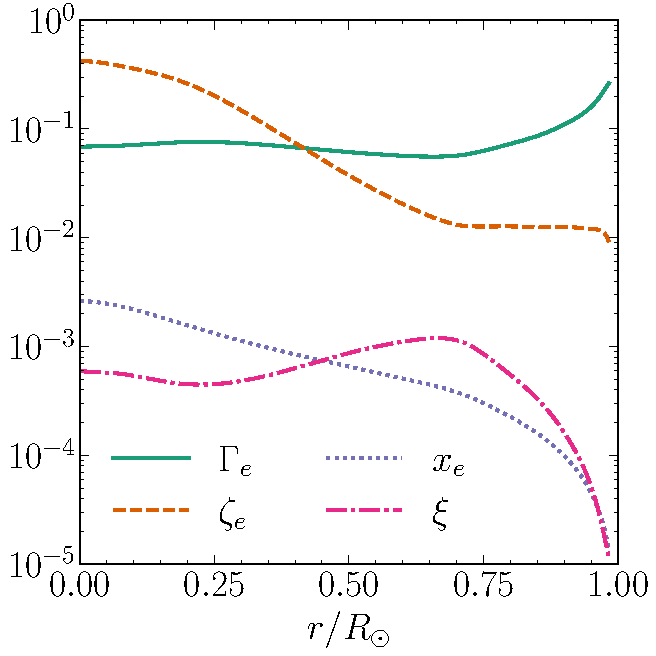
\includegraphics[width=0.5\linewidth]{Solar Model Images/weird_stuff.pdf}
    \caption{Profiles of the importance of Coulomb interactions $\Gamma_e$, degeneracy $\zeta_e$, relativistic energy $x_e$, and radiation pressure $\xi$ within the Sun calculated using the solar model in Ref.~\cite{Bahcall_2005}.}
    \label{fig:weird_stuff}
\end{figure}

Out of the phenomena discussed here, the partial degeneracy of electrons near the solar core is of moderate importance. Coulomb interactions between electrons are of modest importance throughout the Sun, with the contributions from relativistic behavior and radiation pressure being negligible.

\pagebreak

\setcounter{equation}{0}
\section{Maxwell-Boltzman Distribution} \label{ap:MB_dist}
The Maxwell-Boltzmann distribution describes the velocities of non-interacting, non-relativistic, classical particles in thermodynamic equilibrium. The distribution of particles with mass $m$ and velocity $v$ at a temperature $T$ is given by

\begin{equation}
    f(v) = 4\pi v^2 \bigparenthesis{\frac{m}{2\pi k_\mathrm{B}T}}^{3/2} \exp \bigparenthesis{-\frac{mv^2}{2k_\mathrm{B}T}}.
\end{equation}
%
For nuclear reactions within stars, the velocities of particles $a$ and $b$ are both described by independent Maxwell-Boltzmann distributions. That is,

\begin{align}
    f(v_a) &= 4\pi v_a^2 \bigparenthesis{\frac{m_a}{2\pi k_\mathrm{B}T}}^{3/2} \exp \bigparenthesis{-\frac{m_a v_a^2}{2k_\mathrm{B}T}}\text{ and} \\
    f(v_b) &= 4\pi v_b^2 \bigparenthesis{\frac{m_b}{2\pi k_\mathrm{B}T}}^{3/2} \exp \bigparenthesis{-\frac{m_b v_b^2}{2k_\mathrm{B}T}}.
\end{align}
%
The reaction rate per particle pair, $\left<\sigma v\right>$, involves integrating over each velocity distribution by

\begin{equation}
    \left<\sigma v\right> = \int_0^\infty \int_0^\infty f(v_a)f(v_b) \sigma(v_\mathrm{rel})v_\mathrm{rel} dv_a dv_b,
\end{equation}
%
where $v_\mathrm{rel}$ is the relative velocity between particles $a$ and $b$. One can transform to the center-of-mass (com) frame of this two-particle system using

\begin{align}
    v_\mathrm{rel} &= |v_a - v_b|, \\
    v_\mathrm{com} &= \frac{m_a v_a + m_b v_b}{m_a + m_b}, \\
    m_r &= \frac{m_a m_b}{m_a + m_b},\text{ and} \\
    m_\mathrm{tot} &= m_a + m_b,
\end{align}
%
where $v_\mathrm{com}$ is the velocity of the center of mass, $m_r$ is the reduced mass, and $m_\mathrm{tot}$ is the total mass. This allows for writing distributions for both the relative and center-of-mass velocities:

\begin{align}
    f(v_\mathrm{rel}) &= 4\pi v_\mathrm{rel}^2 \bigparenthesis{\frac{m_r}{2\pi k_\mathrm{B}T}}^{3/2} \exp\bigparenthesis{-\frac{m_r v_\mathrm{rel}^2}{2k_\mathrm{B}T}} \\
    f(v_\mathrm{com}) &= 4\pi v_\mathrm{com}^2 \bigparenthesis{\frac{m_\mathrm{tot}}{2\pi k_\mathrm{B}T}}^{3/2} \exp\bigparenthesis{-\frac{m_\mathrm{tot} v_\mathrm{com}^2}{2k_\mathrm{B}T}}
\end{align}
%
Conversely,

\begin{equation}
    \left<\sigma v\right> = \int_0^\infty \int_0^\infty f(v_\mathrm{com})f(v_\mathrm{rel}) \sigma(v_\mathrm{rel})v_\mathrm{rel} dv_\mathrm{com} dv_\mathrm{rel}.
\end{equation}
%
The nuclear cross section depends only on relative velocities between particles, the integration over $v_\mathrm{com}$ is trivially performed, since the Maxwell-Boltzmann distribution is normalized, yielding

\begin{equation}
    \left<\sigma v\right> = \int_0^\infty f(v_\mathrm{rel}) \sigma(v_\mathrm{rel})v_\mathrm{rel} dv_\mathrm{rel}.
\end{equation}
%
Dropping subscripts and inserting the Maxwell-Boltzmann distribution,

\begin{equation}
    \left<\sigma v\right> = 4\pi \bigparenthesis{\frac{m_r}{2\pi k_\mathrm{B}T}}^{3/2} \int_0^\infty v^3 \sigma(v) \exp\bigparenthesis{-\frac{m_r v^2}{2k_\mathrm{B}T}} dv.
\end{equation}
%
In terms of the energy $E = \frac{1}{2}m_r v^2$, 

\begin{empheq}[box=\fbox]{equation}
    \left<\sigma v\right>  = \bigparenthesis{\frac{8}{\pi m_r}}^{1/2} \frac{1}{(k_\mathrm{B}T)^{3/2}} \int_0^\infty \sigma(E) E \exp\bigparenthesis{-\frac{E}{k_\mathrm{B}T}} dE. \label{eq:ap_mb_sigmav}
\end{empheq}

\pagebreak

\setcounter{equation}{0}
\section{Ideal Gas Law} \label{ap:ideal_gas}
This Appendix contains additional details regarding the ideal gas law and thermodynamics. A useful table of the Maxwell relations is given in Figure \ref{fig:MW_relations}.

\begin{figure}[H]
    \centering
    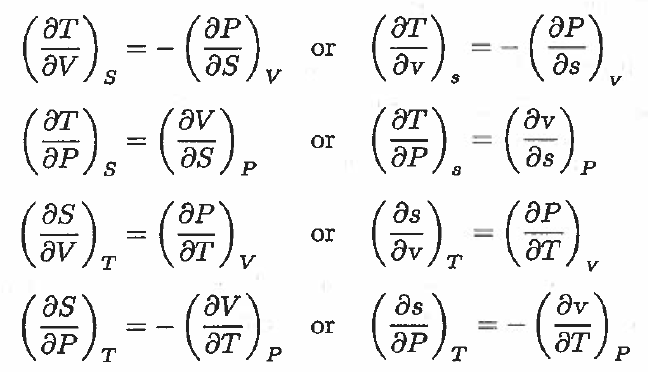
\includegraphics[width=0.5\linewidth]{Appendices//Ideal Gas Law/Maxwell_relations.png}
    \caption{Maxwell relations, taken from~\cite{EracleousPSU}. Quantities in lowercase denote specific (per unit mass) versions of general quantities. For example, $S$ is entropy, while $s$ is specific entropy.}
    \label{fig:MW_relations}
\end{figure}

\subsection{Thermodynamic Properties} \label{ap:ideal_gas_thermo_prop}
The ideal gas law comes in many forms for use in different fields or contexts. As an equation of state, it is frequently expressed as

\begin{equation}
    P = n k_\mathrm{B}T = \frac{\mathcal{R}}{\mu} \rho T = \frac{\rho}{\mu m_a} k_B T
\end{equation}
%
where $P$ is pressure, $n$ is number density, $k_\mathrm{B}$ is the Boltzmann constant, $T$ is temperature, $\mathcal{R}$ is the universal gas constant (units of energy per Kelvin per unit mass), $\mu$ is the mean molecular weight, $m_a$ is the atomic mass unit, and $\rho$ is the mass density.

The isothermal compressibility coefficient for an ideal gas is 

\begin{equation}
    \alpha = \frac{P}{\rho}\bigparenthesis{\pderiv{\rho}{P}}_{T,\mu} =  \frac{\mathcal{R}\rho T/\mu}{\rho} \bigparenthesis{\frac{\mu}{\mathcal{R}T}} = 1.
\end{equation}
%
The coefficient of expansion for an ideal gas is

\begin{equation}
    \delta = -\frac{T}{\rho} \bigparenthesis{\pderiv{\rho}{T}}_{T,\mu} = -\frac{T}{P\mu/(\mathcal{R}T)} \bigparenthesis{-\frac{P\mu}{\mathcal{R}T^2}} = 1.
\end{equation}
%
We can find the specific heats (or heat capacities) of an ideal gas using relations equivalent to those in Appendix \ref{ap:equations} given by

\begin{align}
    c_P &\equiv \bigparenthesis{\pderiv{q}{T}}_{P} = T\bigparenthesis{\pderiv{s}{T}}_{P}\text{ and} \\
    c_V &\equiv \bigparenthesis{\pderiv{q}{T}}_V = T\bigparenthesis{\pderiv{s}{T}}_V
\end{align}
%
where $q$ is specific heat content, $s$ is specific entropy, $P$ is pressure, $V$ is volume, and $c$ are specific heats. The ratio of specific heats,

\begin{equation}
    \gamma \equiv \frac{c_P}{c_V},
\end{equation}
%
is known as the adiabatic index. For a classical gas, the adiabatic index can be determined by the number of degrees of freedom $f$ available to the particles of the gas:

\begin{equation}
    \gamma = 1 + \frac{2}{f}
\end{equation}
%
For a monatomic gas with three translational degrees of freedom, $\gamma = 5/3$.

The specific heats can be related starting from the second law of thermodynamics:

\begin{equation}
    dq = T ds
\end{equation}
%
After making the assumption that entropy is a function of temperature and pressure, we can write the second law as

\begin{equation}
    dq = T \left(\bigparenthesis{\pderiv{s}{T}}_P dT + \bigparenthesis{\pderiv{s}{P}}_T dP \right).
\end{equation}
%
If we also assume that pressure is a function of temperature and (specific) volume $v$, we can write

\begin{equation}
    dP = \bigparenthesis{\pderiv{P}{T}}_v dT + \bigparenthesis{\pderiv{P}{v}}_T dv.
\end{equation}
%
Inserting the above equation into the second law of thermodynamics, we obtain

\begin{equation}
    dq = T \left(\bigparenthesis{\pderiv{s}{T}}_T dT + \bigparenthesis{\pderiv{s}{P}}_T \bigparenthesis{\pderiv{P}{T}}_v dT + \bigparenthesis{\pderiv{s}{P}}_T \bigparenthesis{\pderiv{P}{v}}_T dv \right).
\end{equation}
%
In looking for the specific heat at constant volume, we may set $dv = 0$ and divide the above equation by dT. This works out as

\begin{equation}
    \bigparenthesis{\pderiv{q}{T}}_v = T\bigparenthesis{\pderiv{s}{T}}_P + T \bigparenthesis{\pderiv{s}{P}}_T \bigparenthesis{\pderiv{P}{T}}_v. \label{eq:ap_ideal_gas_algebra1}
\end{equation}
%
From the definitions of thermodynamic quantities and the usual Maxwell's relations, we can identify three expressions in the above equation,

\begin{align}
    \bigparenthesis{\pderiv{q}{T}}_v &= c_V, \\
    T \bigparenthesis{\pderiv{s}{T}}_P &= c_P,\text{ and} \\
    \bigparenthesis{\pderiv{s}{P}}_T &= -\bigparenthesis{\pderiv{v}{T}}_P,
\end{align}
%
which we can then replace in Equation \ref{eq:ap_ideal_gas_algebra1} to obtain

\begin{equation}
    c_P - c_V = T\bigparenthesis{\pderiv{v}{T}}_P \bigparenthesis{\pderiv{P}{T}}_v. \label{eq:ap_ideal_gas_heat_algebra}
\end{equation}
%
The first differential can be rewritten in terms of the coefficient of expanison:

\begin{equation}
    T\bigparenthesis{\pderiv{v}{T}}_P = v\delta = \frac{\delta}{\rho}.
\end{equation}
%
To rewrite the second differential, we again keep in mind that volume is kept constant:

\begin{align}
    dv = 0 &= \bigparenthesis{\pderiv{v}{T}}_P + \bigparenthesis{\pderiv{v}{P}}_T \\
    \bigparenthesis{\pderiv{v}{T}}_P &= -\bigparenthesis{\pderiv{v}{P}}_T \\
    \bigparenthesis{\pderiv{P}{T}}_v &= -\bigparenthesis{\pderiv{v}{T}}_P \big/ \bigparenthesis{\pderiv{v}{P}}_T \label{eq:ap_ideal_gas_algebra2}
\end{align}
%
where, again, we can identify 

\begin{align}
    \bigparenthesis{\pderiv{v}{T}}_P &= \frac{\delta}{\rho T}\text{ and} \\
    \bigparenthesis{\pderiv{v}{P}}_T &= \alpha.
\end{align} 
%
to plug in Equation \ref{eq:ap_ideal_gas_algebra2} to obtain

\begin{equation}
    \bigparenthesis{\pderiv{P}{T}}_v = \frac{P\delta}{T\alpha}.
\end{equation}
%
When combining the above with Equation \ref{eq:ap_ideal_gas_heat_algebra}, we arrive at

\begin{equation}
    c_P - c_V = \frac{P\delta^2}{T\rho \alpha}. \label{eq:ap_ideal_gas_heat_algebra2}
\end{equation}
%
For an ideal gas, the equation of state can be expressed as 

\begin{equation}
    P = \frac{\rho}{\mu m_a} k_B T
\end{equation}
%
Which, when substituted into Equation \ref{eq:ap_ideal_gas_heat_algebra}, gives

\begin{equation}
    c_P - c_V = \frac{k_B}{\mu m_a} = \mathscr{R},
\end{equation}
%
where $\mathscr{R}$ is the \textit{molar} gas constant, used in the well-known $PV = N\mathscr{R}T$ equation for the ideal gas law.

Reintroducing the adiabatic index, we can write

\begin{equation}
    c_P - c_V = \left(\frac{c_P}{c_V} - 1 \right) = \left(\gamma - 1 \right) c_V.
\end{equation}
%
which allows for finally obtaining expressions for the specific heats:

\begin{align}
    c_V &= \frac{1}{\gamma-1} \frac{k_\mathrm{B}}{\mu m_a} \\
    c_P &= \frac{\gamma}{\gamma - 1} \frac{k_\mathrm{B}}{\mu m_a}
\end{align}

\subsection{Adiabatic Equation of State} 
Here I reproduce a derivation of the equation of state for a gas undergoing an adiabatic process.

The second law of thermodynamics states

\begin{equation}
    dq = Tds = du + Pdv = du - \frac{P}{\rho^2}d\rho.
\end{equation}
%
For a gas that is conserving its heat content, $dv = 0$, giving

\begin{equation}
    du = dq = c_V dT. \label{eq:ap_ad_eos1}
\end{equation}
%
Furthermore, the second law also relates

\begin{equation}
    du = Tds + \frac{P}{\rho^2} d\rho.
\end{equation}
%
For an adiabatic process, $ds = 0$ and so

\begin{equation}
    du = \frac{P}{\rho^2} d\rho. \label{eq:ap_ad_eos2}
\end{equation}
%
Setting Equations \ref{eq:ap_ad_eos1} and \ref{eq:ap_ad_eos2} equal,

\begin{equation}
    c_V dT = \frac{P}{\rho^2} d\rho.  \label{eq:ap_ad_eos3}
\end{equation}
%
Starting from the equation of state of an ideal gas, we can find an expression for $dT$:

\begin{align}
    P &= \frac{\rho}{\mu m_a} k_\mathrm{B} T \\
    T &= \frac{P\mu m_a}{\rho k_\mathrm{B}} \\
    dT &= \frac{\mu m_a}{k_\mathrm{B}} \left(\frac{dP}{\rho} - P\frac{d\rho}{\rho^2} \right) \label{eq:ap_ad_eos4}
\end{align}
%
Combining Equations \ref{eq:ap_ad_eos3} and \ref{eq:ap_ad_eos4}, we obtain

\begin{align}
    c_V \bigparenthesis{\frac{\mu m_a}{k_\mathrm{B}}} \bigparenthesis{\frac{dP}{\rho} - P\frac{d\rho}{\rho^2}} = \frac{P}{\rho^2} d\rho \\
    c_V \bigparenthesis{dP - P\frac{d\rho}{\rho}} - \frac{k_\mathrm{B}}{\mu m_a} P \frac{d\rho}{\rho} = 0 \\
    c_V dP - c_V P \frac{d\rho}{\rho} - \frac{k_\mathrm{B}}{\mu m_a} P \frac{d\rho}{\rho} = 0.
\end{align}
%
Since $c_P - c_V = \frac{k_\mathrm{B}}{\mu m_a}$,

\begin{align}
    c_V dP - c_V P \frac{d\rho}{\rho} - \left(c_P - c_V\right) P \frac{d\rho}{\rho} - 0 \\
    c_V dP - c_V P \frac{d\rho}{\rho} - c_P P \frac{r\rho}{\rho} + c_V P \frac{d\rho}{\rho} = 0 \\
    c_V dP - c_P P \frac{d\rho}{\rho} = 0 \\
    \frac{dP}{P} = \frac{c_P}{c_V} \frac{d\rho}{\rho} \\
    \frac{dP}{P} = \gamma \frac{d\rho}{\rho}. \label{eq:ap_eos_diffyq}
\end{align}
%
In Equation \ref{eq:ap_eos_diffyq} we have serendipitously arrived at a separated differential equation relating pressure and density. Upon integration, one obtains

\begin{equation}
    P \propto \rho^\gamma.
\end{equation}
%
If one is in need of the adiabatic equation of state in terms of specific internal energy $u$,

\begin{align}
    du &= c_V dT \\
    du &= \frac{1}{\gamma - 1}\frac{k_\mathrm{B}}{\mu m_a} dT \\
    du &= \frac{1}{\gamma - 1} \bigparenthesis{\frac{dP}{\rho} - P\frac{d\rho}{\rho^2}} \\
    du &= \frac{1}{\gamma - 1} d\bigparenthesis{\frac{P}{\rho}}.
\end{align}
%
Upon integration, we obtain

\begin{equation}
    P = (\gamma - 1) \rho u.
\end{equation}

\subsection{Adiabatic Temperature Gradient} \label{ap:nabla_ad_ideal}
Useful to the discussion of energy transport is the adiabatic temperature gradient given by

\begin{equation}
    \nabla_\mathrm{ad} = \frac{P\delta}{T\rho c_P}.
\end{equation}
%
By plugging in

\begin{align}
    P &= \frac{\rho}{\mu m_a} k_\mathrm{B} T, \\
    \delta &= 1 \text{ (for an ideal gas), and} \\
 c_P &= \frac{\gamma}{\gamma - 1} \frac{k_\mathrm{B}}{\mu m_a},    
\end{align}
%
one obtains

\begin{equation}
    \nabla_\mathrm{ad} = \frac{\gamma - 1}{\gamma}.
\end{equation}
%
For a monatomic ideal gas with $\gamma = \frac{5}{3}$,

\begin{empheq}[box=\fbox]{equation}
\nabla_\mathrm{ad} = \frac{2}{5}.
\end{empheq}

\pagebreak

\setcounter{equation}{0}
\section{Nuclear Fusion} \label{ap:fusion}
This Appendix contains additional details regarding nuclear fusion reactions.

\subsection{Nuclear Reactions in the Sun} \label{ap:nucReac}

Figure \ref{fig:pp_reactions_psu} showcases the main nuclear reactions of the pp chain, the energy per nucleon liberated from the termination of each sub-chain, and the characteristic timescale for each reaction. 

\begin{figure}[H]
    \centering
    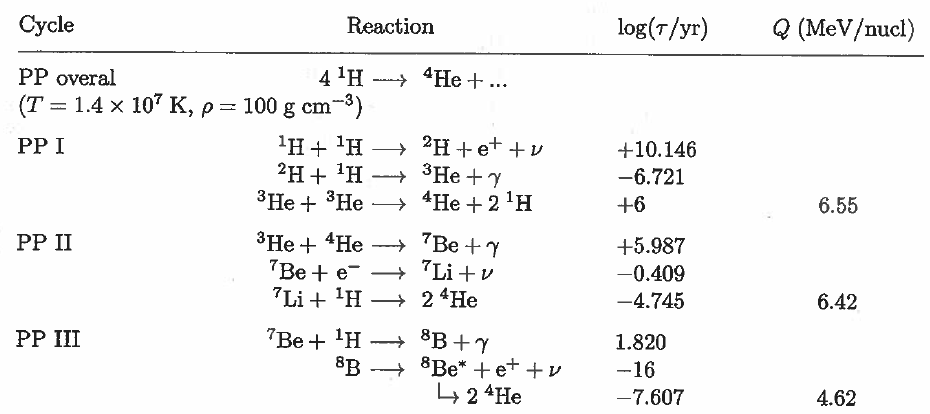
\includegraphics[width=0.6\linewidth]{Appendices//Nuclear Fusion/PP_reactions.png}
    \caption{Table of selected reactions of the pp chain taken from~\cite{EracleousPSU}.}
    \label{fig:pp_reactions_psu}
\end{figure}

\begin{figure}[H]
    \centering
    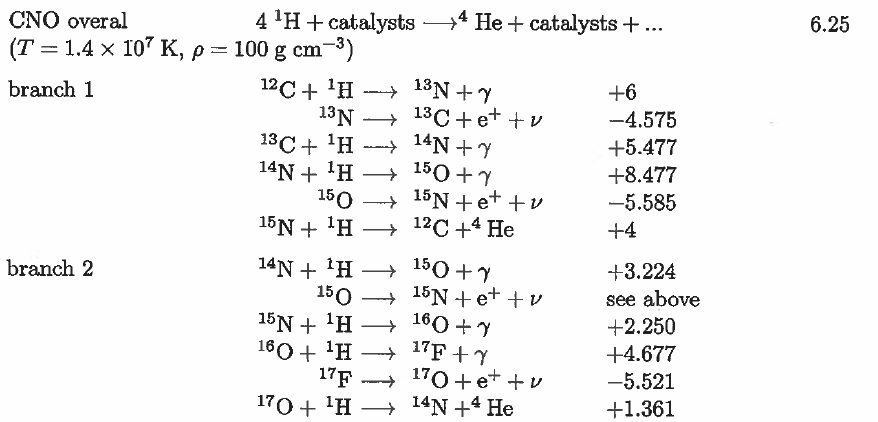
\includegraphics[width=0.6\linewidth]{Appendices//Nuclear Fusion/CNO_reactions.png}
    \caption{Same as Figure \ref{fig:pp_reactions_psu} but for the CNO bi-cycle.}
    \label{fig:CNO_reactions_psu}
\end{figure}

For a species $a$ involved in reactions with species $b$, one may define a characteristic lifetime for $a$ specific to reactions with $b$ via

\begin{equation}
    \deriv{n_a}{t} = \Gamma_{ab} = -\frac{n_a}{\tau_{ab}}
\end{equation}
%
where $\Gamma_\mathrm{ab}$ is the reaction rate between $a$ and $b$. The lifetimes quoted in Figures \ref{fig:pp_reactions_psu} and \ref{fig:CNO_reactions_psu} correspond to harmonic sums of species on the left-hand-side of each reaction in the Sun.

One may consider the many orders of magnitude in timescales spanned by the various reactions, and note that the fusion of two protons ($^{1}$H + $^{1}$H $\rightarrow$ $^{2}$H + e$^{+} + \nu$) limits the overall rate of the pp chain. This is because a short-lived intermediate state is formed, the diproton ($^2$He), during which a beta decay must occur for the reaction to proceed:

\begin{equation}
    ^1 \mathrm{H} +\text{} ^1\mathrm{H} \longleftrightarrow \text{} ^2\mathrm{He} \stackrel{\beta+}{\longrightarrow}\text{} ^2\mathrm{H} + e^+ + \nu_\mathrm{e}
\end{equation}
%
The beta decay actually occurs in one out of $10^{27}$ diprotons formed~\cite{Cox_Giuli_vol1}, a consequence of the weak interaction. This is reflected in the extremely small value for the astrophysical $S_{11}$ factor compared to the rest of the pp chain and CNO bi-cycle, showcased in Figure \ref{fig:s_table} from Ref.~\cite{Acharya2024}.

\begin{figure}[H]
    \centering
    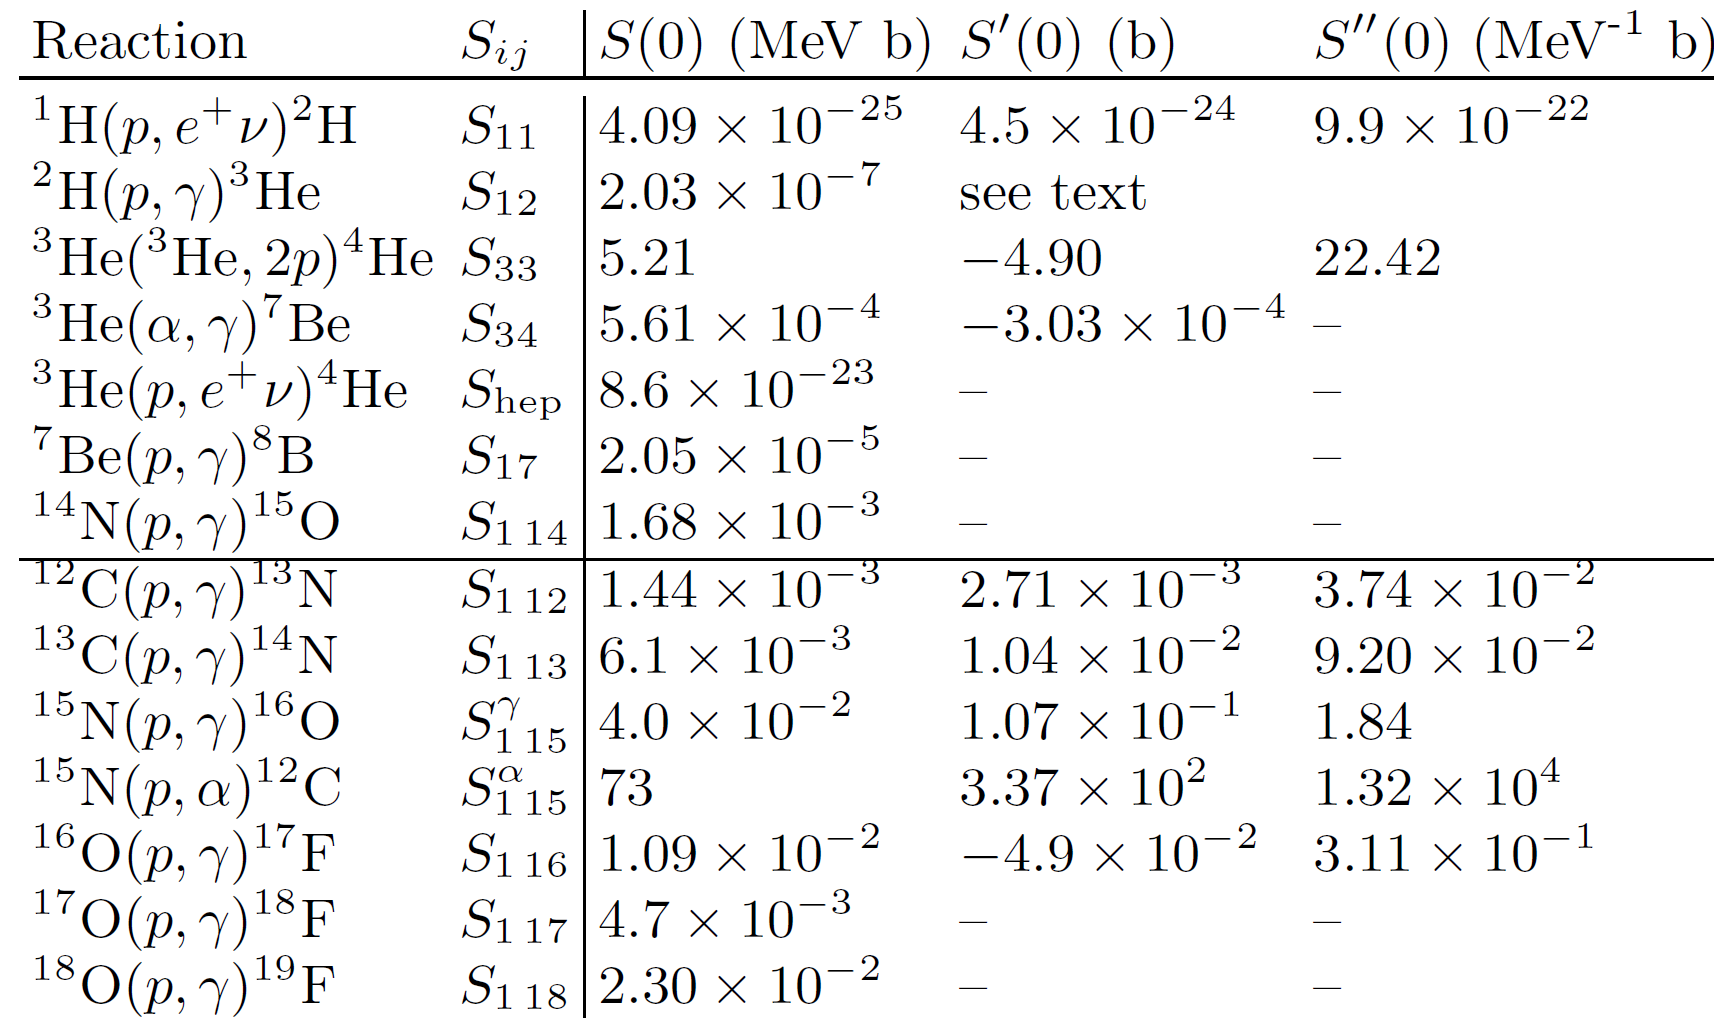
\includegraphics[width=0.75\linewidth]{Appendices//Nuclear Fusion/S_factors.png}
    \caption{S factors and derivatives for the reactions of the pp chain and CNO cycle taken from~\cite{Acharya2024}.}
    \label{fig:s_table}
\end{figure}

Note that the \textit{hep} reaction also proceeds via the weak interaction, having a much smaller value of $S$ than other reactions. For the purposes of generating figures in the main text of this report, any values of $S$, $S'$, and $S''$ not provided in Figure \ref{fig:s_table} were set equal to zero.

\subsection{Details of Nuclear Reaction Rates} \label{ap:rates}
In this subsection, I provide more details regarding the computation of nuclear reaction rates as described in the main text. I follow along with the arguments in Chapter 4 of Ref.~\cite{Phillips1999}, Chapter 6 of Ref.~\cite{HK_book}, Chapter 3 of Ref.~\cite{Rolfs1988}, and others.

Consider an interaction between two nuclei with atomic numbers $Z_a$ and $Z_b$ and masses $m_a$ and $m_b$. The electrostatic potential energy between the nuclei separated by a distance $r$ is given by

\begin{equation}
    E = \frac{Z_a Z_b e^2}{4\pi \epsilon_0 r}.
\end{equation}
%
This energy is positive, and so is a potential barrier which particles must overcome in order to fuse. The strong nuclear interaction is very attractive on length scales comparable to size of nuclei $r_N$, which may be estimated by

\begin{equation}
    r_N \approx 1.4 \times 10^{-15} A^{1/3}  \text{ m}
\end{equation}
%
where $A$ is the mass number of a nucleus. When $r \sim r_N$, the strong nuclear interaction takes over, and fusion occurs. The minimum interpacticle separation between nuclei, $R$, is given by

\begin{equation}
    R = 1.4 (A_a^{1/3} + A_X^{1/3}) \text{ fm}
\end{equation}
%
corresponding to a Coulomb barrier height of 

\begin{equation}
    E_C = \frac{Z_a Z_b e^2}{4\pi \epsilon_0 R} = 1.44 Z_a Z_b \bigparenthesis{\frac{R}{1 \text{ fm}}}^{-1} \text{ MeV}.
\end{equation}
%
In the Sun, the central temperature is of order $10^7$ K, which corresponds to thermal energies $E \sim k_\mathrm{B}T \approx 900$ eV, far below the height of the Coulomb barrier. Using the Maxwell-Boltzmann distribution, we can determine the proportion of particles in the Sun that may have such energies. The distribution is given by

\begin{equation}
    f(E) = 2\sqrt{\frac{E}{\pi}} \bigparenthesis{\frac{1}{k_\mathrm{B}T}}^{3/2} \exp\bigparenthesis{-\frac{E}{k_\mathrm{B}T}},
\end{equation}
%
and the fraction $f'$ of particles which have the necessary energy is given by

\begin{equation}
    f' = \int_{E_C}^{\infty} dE f_E(E).
\end{equation}
%
For the fusion of two protons with $Z_a = Z_b = 1$ and $A = 1$, $E_C \approx 1.02$ MeV, $f' \approx 2 \times 10^{-481}$. There are not nearly enough particles in the universe to even write out such a number.

Consider Figure \ref{fig:fusion_potential}.

\begin{figure}[H]
    \centering
    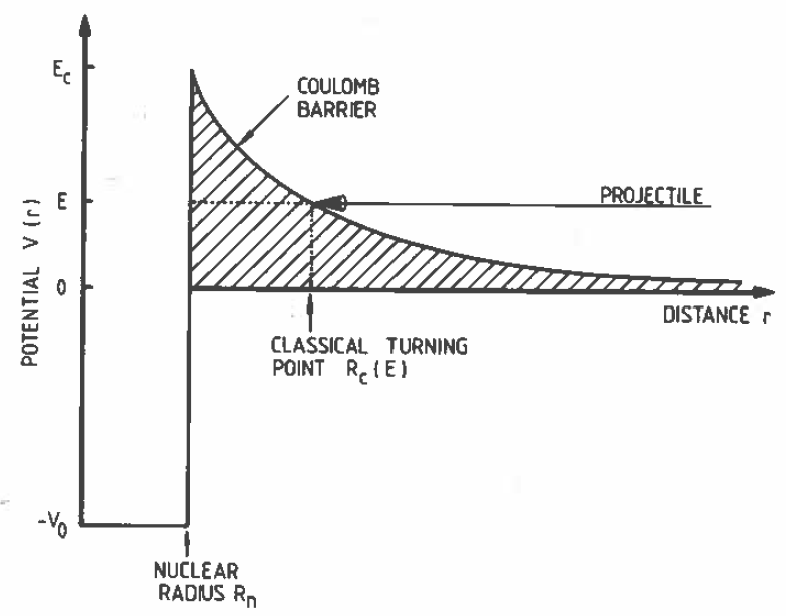
\includegraphics[width=0.5\linewidth]{Appendices//Nuclear Fusion/potential_barrier.png}
    \caption{Schematic representation of the potential experienced by a projectile when interacting with a target to fuse~\cite{Rolfs1988}.}
    \label{fig:fusion_potential}
\end{figure}

In a one-dimensional quantum mechanical treatment of this problem, a projectile nucleus with energy $E$ can reach a distance $R_c$ from a target called the classical turning point, given by the formula for electrostatic potential energy. The probability to find the projectile within some small window $\delta$ of $R_c$ is given by

\begin{equation}
    \text{p}(R_c - \delta \leq r \leq R_c + \delta) = \int_{R_c - \delta}^{R_c + \delta} |\psi(r)|^2 dr
\end{equation}
%
where $\psi(r)$ is the position space wave function of the projectile. On the other side of the Coulomb barrier, the strong nuclear force takes over at a distance $R_N$, at which the wave function has a value $\psi(R_c)$. The ratio of the probability amplitude at the nuclear radius to that at the classical turning point gives the probability that the target tunnels through the Coulomb barrier and fuses:

\begin{equation}
    \text{p}(\text{tunnel}) = \frac{|\psi(R_n)|^2}{|\psi(R_c)|^2}
\end{equation}
%
Solving the Schr{\"o}dinger equation produces this probability~\cite{Rolfs1988}, giving

\begin{equation}
    \text{p}(\text{tunnel}) =  \exp \bigparenthesis{-2\bigparenthesis{\frac{2m_r}{\hbar^2}(E_C - E)}^{1/2} R_c \left[\frac{\arctan(R_c/R_n - 1)^{1/2}}{(R_c/R_n - 1)^{1/2}} - \frac{R_n}{R_c} \right]},
\end{equation}
%
where $m_r$ is the reduced mass of the projectile and target. If $R_c >> R_n$, or equivalently, $E<<E_c$, the tunneling probability reduces to 

\begin{equation}
    \text{p}(\text{tunnel}) \approx \exp\bigparenthesis{-\sqrt{\frac{E_G}{E}}}
\end{equation}
%
where $E_G = 2m_r c^2 (\pi \alpha Z_a Z_b)$ is the Gamow energy in the CGS units ($\alpha = e^2/\hbar c$). In the literature, the tunneling probability is usually written as

\begin{equation}
    \exp\bigparenthesis{-\sqrt{\frac{E_G}{E}}} = \exp\bigparenthesis{-2\pi\eta}, \label{eq:gamow_Factor}
\end{equation}
%
where $\eta = Z_a Z_b \frac{e^2}{h} \sqrt{\frac{m_r}{2E}}$ is the Sommerfield parameter, and the right-hand-side of Equation \ref{eq:gamow_Factor} is called the Gamow factor.

Below the Coulomb barrier, the cross section for charged-particle induced nuclear reactions drops rapidly~\cite{Rolfs1988} as

\begin{equation}
    \sigma(E) \propto \exp \bigparenthesis{-2\pi\eta}.
\end{equation}
%
In addition, cross sections also depend on the energetics outside of the realm of nuclear physics. One can write an energy-dependent cross section in terms of the de Broglie wavelength 

\begin{equation}
\lambda = \frac{\hbar}{\sqrt{2m_a E_a}}    
\end{equation}
%
of the projectile particle as

\begin{equation}
    \sigma(E) \propto \pi \lambda^2 \propto \frac{1}{E}.
\end{equation}
%
The remaining nuclear physics to be measured via experiment is packaged into the astrophysical S factor $S(E)$, arriving at

\begin{equation}
    \sigma(E) = \frac{S(E)}{E}\exp\bigparenthesis{-2\pi\eta}.
\end{equation}
%
I now derive the expression for the rate of nuclear reactions from simple arguments. Within a region of interest there may be $n_a$ particles per cubic centimeter of nuclear species $a$ and $n_b$ particles per cubic centimeter of nuclear species $b$. These particles have relative velocities $v$, and the center-of-mass velocities are not relevant for nuclear reactions. As such, either species of particle may be treated as a ``projectile" in motion, with the other at rest as a ``target".

We may arbitrarily choose species $a$ as the projectiles, which stream along and ``see" an effective reaction area $F$ given by

\begin{equation}
    F = \sigma(v)n_b.
\end{equation}
%
This may be understood as an inverse mean-free-path, i.e., the typical length scale that a projectile travels before interacting with a target. Each projectile in the region of interest experiences an identical effective reaction area, and so the number of nuclear reactions must depend on the flux of incident particles $J$ given by

\begin{equation}
    J = n_a v.
\end{equation}
%
The rate of nuclear reactions $\Gamma$ is finally the product of the reaction area and the flux of incident projectiles:

\begin{equation}
    \Gamma = FJ = n_a n_b v \sigma(v)
\end{equation}
%
For identical particle pairs, this product is a factor of two too large, which may be solved by the inclusion of a $(1 + \delta_{ab})$ factor in the denominator. Still, since the velocities of particles takes a range of values at finite temperature, the reaction rate per particle pair must be averaged over the velocity distribution as 

\begin{equation}
    \sigma(v)v \longrightarrow \left< \sigma v\right> = \int_0^\infty f(v) v \sigma(v) dv
\end{equation}
%
where $f(v)$ is the Maxwell-Boltzmann velocity distribution. 

Combining everything in terms of the center of mass energy, the rate of nuclear reactions per cubic centimeter per second is given by

\begin{empheq}[box=\fbox]{equation}
    \Gamma_{ab}  = \frac{n_a n_b}{1 + \delta_{ab}}\bigparenthesis{\frac{8}{\pi m_r}}^{1/2} \frac{1}{(k_\mathrm{B}T)^{3/2}} \int_0^\infty S(E) \exp\bigparenthesis{-\frac{E}{k_\mathrm{B}T} - 2\pi\eta} dE. \label{abba}
\end{empheq}


\subsection{Reaction Rate Approximation in the Sun} \label{ap:SunRates}
In the main text of my report I compute non-resonant contributions to nuclear reaction rates in the Sun from an approximate formula presented in Ref.~\cite{bahcall1989neutrino}. For a discussion on how to derive such an approximation, see Chapters 17.13 and 17.15 in Ref.~\cite{Cox_Giuli_vol1}.

A convenient form for the reaction rate per particle pair is given by

\begin{equation}
    \left<\sigma v\right> = 1.3005\times10^{-15} \left[ \frac{Z_a Z_b}{A T_6^2}\right]^{1/3} f_0 S_\mathrm{eff} \exp(-\tau) \text{ cm}^3 \text{ s}^{-1}.
\end{equation}
%
I provide definitions of each quantity below.

\begin{itemize}
    \item $Z_i$ are the atomic numbers of the species involved,
    \item $A$ is the reduced atomic mass of the species in amu, given by $A = (A_a A_b)/(A_a + A_b)$
    \item $T_6 = T/(10^6\text{ K})$, the temperature $T$ in units of millions of Kelvin,
    \item $f_0 = \exp\bigparenthesis{0.188Z_a Z_b \zeta \rho^{1/2} T_6^{-3/2}}$ is a factor accounting for the screening of electrons,
    \item $\zeta = \left[\sum_i (X_i Z_i^2 /A_i + X_i Z_i/A_i) \right]^{1/2}$ has no particular name,
    \item $\rho$ is the mass density expressed in implicit units of g cm$^{-3}$,
    \item $S_\mathrm{eff} = S_\mathrm{eff}(E_0) \approx S(0) \left[1 + \frac{5}{12\tau} + \frac{S' (E_0 + \frac{35}{36}k_\mathrm{B}T)}{S} + \frac{S'' E_0}{S} \left(\frac{E_0}{2} + \frac{89}{72}k_\mathrm{B}T \right) \right]_{E = 0}$ is the effective astrophysical S factor,
    \item $E_0 = 1.2204 \left(Z_1^2 Z_2^2 A T_6^2\right)^{1/3} \text{ keV}$ is the most probable energy of interaction corresponding to the tip of the Gamow peak,
    \item $E$ is the center of mass energy of the reaction,
    \item $\tau = 3E_0/(k_\mathrm{B}T) = 42.487 \left(Z_1^2 Z_2^2 A T_6^2\right)^{1/3}$ is a dimensionless parameter convenient for the power series expansion of the S factor
    \item $S(0) = S(E=0)$ is the astrophysical S factor for the reaction at zero energy, typically given in tables such as the one in Figure \ref{fig:s_table}, and
    \item $S' \equiv dS/dE$ and $S'' \equiv d^2 S/dE^2$ are derivatives of the astrophysical S factor, here evaluated at $E = 0$. These are also frequently given in tables.
\end{itemize}

The above approach does not work well for reactions that involve the weak interaction. For example, the so-called \textit{pep} reaction, $\mathrm{p} + \mathrm{e}^{-} + \mathrm{p} \rightarrow \mathrm{d} + \nu_e$, proceeds via an electron capture. The rate of this reaction is described~\cite{Acharya2024} by

\begin{equation}
    \Gamma_\mathrm{pep} = 1.13 \times 10^{-4} (\rho/\mu_e) \times T_6^{-1/2} \times [1 + 0.02(T_6 - 16)] \Gamma_\mathrm{pp}
\end{equation}

where $\rho$ is the usual mass density in implicit cgs units, $\mu_e$ is the mean molecular weight per free electron, and $\Gamma_\mathrm{pp}$ is the reaction rate of the fusion of two protons. Similarly, the electron capture of $^7$Be has an overall rate parameterized~\cite{Acharya2024} by

\begin{equation}
    R_{^7\mathrm{Be} + e^{-}} = 5.60 \times 10^{-9} (\rho/\mu_e) \times T_6^{-1/2} [1 + 0.004(T_6 - 16)] \text{ s}^{-1},
\end{equation}

which is not a volumetric reaction rate like the expressions for $\Gamma$, but can be still calculated throughout the Sun. The literature does not straightforwardly describe why this is not presented as a volumetric reaction rate, and so it is not plotted in the main text of this report.

For fully ionized Hydrogen and Helium, an expression for the average number of free electrons per 1 amu is $\frac{1}{\mu_\mathrm{e}} = \approx \frac{1}{2}(1 + X_\mathrm{H})$, where $X_\mathrm{H}$ is the mass fraction of Hydrogen.

\pagebreak

\setcounter{equation}{0}
\section{Radiative Diffusion and Transport} \label{ap:rad_diff}
This Appendix contains additional details regarding the transport of energy by radiation.
\subsection{Diffusion of Particles}
Consider the diagram in Figure \ref{fig:diff_diagram}.

\begin{figure}[H]
    \centering
    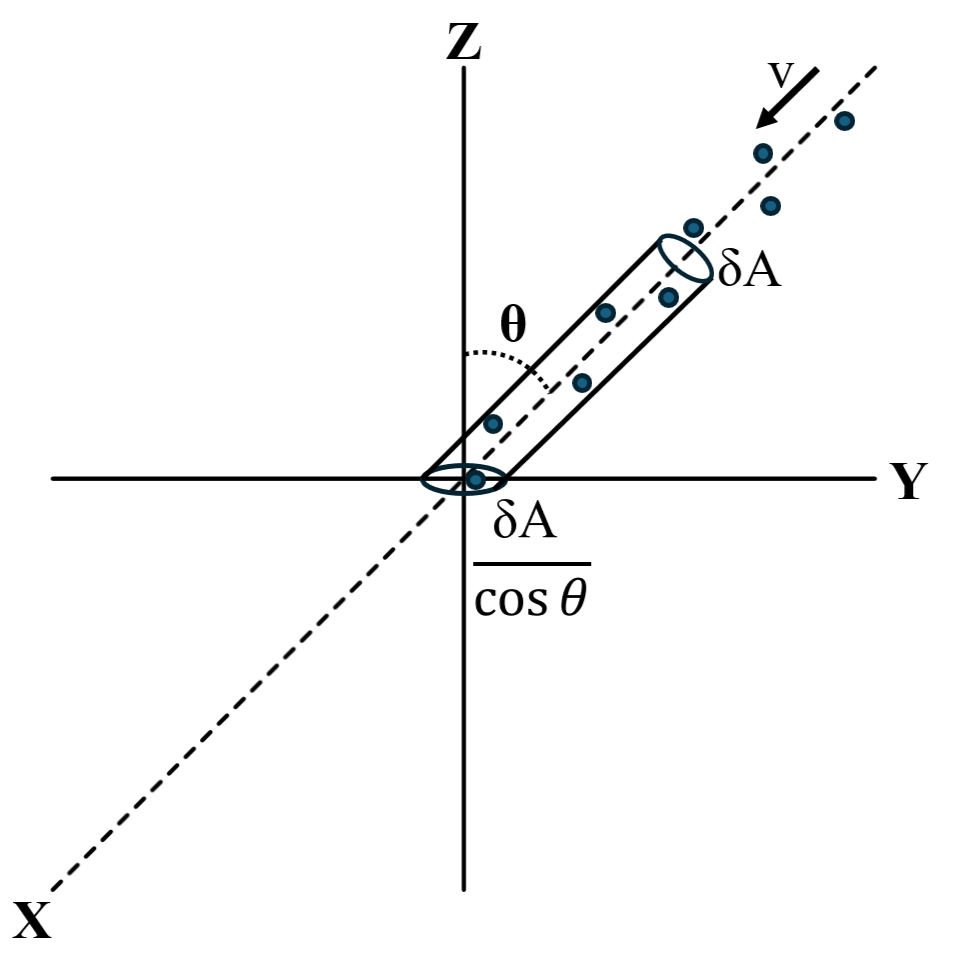
\includegraphics[width=0.5\linewidth]{Appendices//Rad Transport/diffusion.png}
    \caption{A stream of particles with number density $n$ travel at velocity $v$ at an angle $\theta$ with the z-axis and impinge on a target in the x-y plane. The cross sectional area of a fiducial cylinder oriented at angle $\theta$ is $\delta A$, and the area of the target in the x-y plane is $\delta A/\cos\theta$. The length of the fiducial cylinder is $v\delta t$, where $\delta t$ is the time for a particle to reach the target after entering the cylinder.}
    \label{fig:diff_diagram}
\end{figure}

In this setup, the number of particles within the cylinder at a given time is

\begin{equation}
   N_\mathrm{cylinder} = v \text{ } \delta t \text{ } \delta A \text{ } n.
\end{equation}
%
The time required for the particles to reach the target and cross the cylinder is given by

\begin{equation}
    t_\mathrm{cross} = \frac{v \text{ } \delta t}{v\cos\theta}
\end{equation}
%
where the denominator captures the fact that the particles cross the target obliquely. Since the area of the target perpendicular to the x-y plane is $\delta A/\cos\theta$, the flux of particles through the target is given by

\begin{equation}
    \phi = \frac{\text{\# of particles}}{\text{area}\times\text{time}} = \frac{v \text{ } \delta t \text{ } \delta A \text{ } n}{\bigparenthesis{\frac{v \text{ } \delta t}{v\cos\theta}} \bigparenthesis{\frac{\delta A}{\cos\theta}}} = n v \cos^2 \theta.
\end{equation}
%
This flux is for a single orientation of the cylinder, in reality, for particles impinging on the target from a single direction. Integrating over all down-going directions, the total number flux through the target is

\begin{equation}
    \Phi_N = nv \int_0^{\pi/2} \cos^2(\theta) \sin(\theta) d\theta = \frac{1}{3} nv.
\end{equation}

I now move to consider the diffusion of particles within a material. Consider the diagram in Figure \ref{fig:diffusion_mfp}.

\begin{figure}[H]
    \centering
    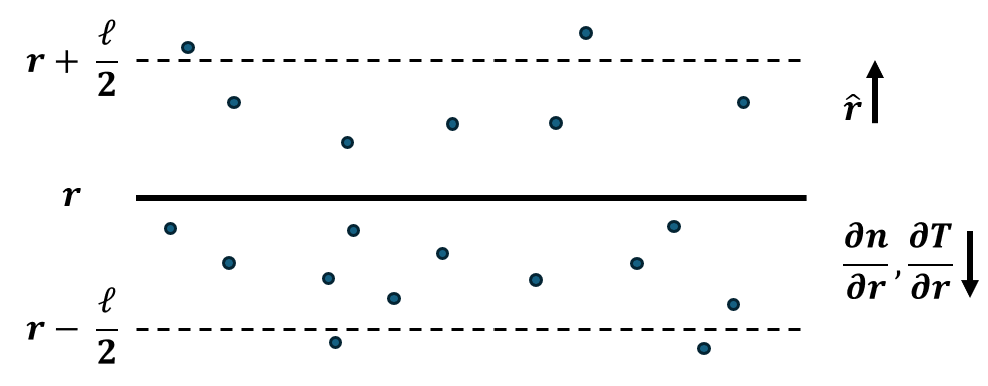
\includegraphics[width=0.5\linewidth]{Appendices//Rad Transport/diffusion2.png}
    \caption{A fiducial surface at radial coordinate $r$ corresponds to a radial shell within a star. Particles in the vicinity of the radial shell move isotropically with a mean velocity $\bar{v}$ and have a number density $n$. Particles typically travel a distance equal to their mean free paths $\ell$ before interacting. Upwards moving particles start at $r - \ell/2$ and travel towards $r + \ell/2$, and vice versa for downward moving particles. The radial direction points up in this figure, meaning temperature $T$ and the number density $n$ of particles increase downwards into the star.}
    \label{fig:diffusion_mfp}
\end{figure}

It is reasonable to imagine that there is a gradient in the quantity $\left<nv\right>$, which may be caused by a gradient in $n$, a gradient in $v$ (due to a temperature gradient), or both. As such, the net flux of particles moving up perpendicular to the surface is given by

\begin{align}
    \Phi_N(r) &= \Phi_\mathrm{up} - \Phi_\mathrm{down} = \frac{1}{3}\left<nv\right>_{r - \ell/2} - \frac{1}{3}\left<nv\right>_{r + \ell/2} \\
    &= \frac{1}{3}\left[\left(\left<nv\right>_r - \frac{\ell}{2}\deriv{}{r}\left<nv\right>_r \right) - \left(\left<nv\right>_r + \frac{\ell}{2}\deriv{}{r}\left<nv\right>_r \right)  \right] \\
    &= -\frac{1}{3}\ell \deriv{}{r}\left<nv\right>.
\end{align}
%
If we assume that the mean velocity of particles $\bar{v}$ changes negligibly around r, 

\begin{equation}
    \Phi_N (r) = -\frac{1}{3} \ell \bar{v} \deriv{n}{r},
\end{equation}
%
which is known as Fick's first law of diffusion with a diffusion coefficient of $D = -\frac{1}{3}\ell \bar{v}$. The resulting flux of energy is obtained by swapping density for energy density $u$:

\begin{equation}
    \Phi_E(r) = -\frac{1}{3} \ell \bar{v} \deriv{u}{r}
\end{equation}
%
The form of $u$ depends on the particles which transport energy.

\subsection{Radiative Transport Equation}
The fundamental quantity describing a radiation field is the specific intensity (also called spectral radiance) $I_\nu$, here parameterized in terms of photon frequency $\nu$. The energy $dE_\nu$ flowing across an area element $dA$ at some position $\vec{r}$ at some time $t$ in a solid angle element $d\Omega$ about a direction $\hat{n}$ in a frequency interval $d\nu$ is given by

\begin{equation}
    dE_\nu  = I_\nu (\vec{r},\hat{n},t) \cos\theta \text{ } d\nu \text{ } dA \text{ } d\Omega \text{ } dt
\end{equation}
%
where $\theta$ is the angle between $\hat{n}$ and the normal direction of the area element. When describing changes in a beam of radiation, one typically uses an equation of radiative transfer. One possible formulation of such an equation is

\begin{equation}
    \frac{1}{c}\pderiv{}{t}I_\nu + \hat{\Omega} \cdot \nabla I_\nu + (\kappa_{\nu, s} + \kappa_{\nu, a})\rho I_\nu = j_\nu \rho + \frac{1}{4\pi} \kappa_{\nu, s} \rho \int_\Omega I_\nu d\Omega \label{eq:ap_transport_eq}
\end{equation}
%
where $c$ is the speed of light, $\hat{\Omega}$ is the normal vector to the area element, $\nabla$ is the gradient operator, $\kappa_{\nu, s}$ is the scattering opacity, $\kappa_{\nu, a}$ is the absorption opacity, $\rho$ is the mass density of the medium in which the beam travels, and $j_\nu$ is the emission coefficient. Starting from the left-hand-side, the first two terms correspond to the continuity of beam and the next describes the scattering and absorption of the beam. On the right-hand-side, the first term describes emission of the medium which adds to the beam, and the final term represents radiation scattered from other directions.

Equation \ref{eq:ap_transport_eq} and similar forms are useful in a careful treatment of radiation in a three-dimensional system with many sources and sinks. For my purposes, I'll consider what happens to a beam in a simple system. Beams can be attenuated by absorption over a distance $s$:

\begin{align}
    dI_\nu &= -a_\nu I_\nu ds \text{, or} \\
    \text{amount lost} &= \text{absorption coefficient} \times \text{beam intensity} \times \text{distance}
\end{align}
%
In this parameterization, the absorption coefficient is a fractional energy loss per unit distance. For an absorbing medium with number density $n$ and cross section with radiation $\sigma_\nu$, one can write the absorption coefficient as

\begin{equation}
    a_\nu = n\sigma_\nu.
\end{equation}
%
The inverse of this quantity is recognizable as the mean free path $\ell_\nu$:

\begin{equation}
    \ell_\nu = \frac{1}{a_\nu}
\end{equation}
%
One can also express the loss of radiation intensity in terms of the opacity $\kappa_\nu$:

\begin{equation}
    \kappa_\nu = \frac{\sigma_\nu}{\mu m_a} = \frac{1}{n\ell_\nu \mu m_a} = \frac{1}{\rho \ell_\nu} = \frac{a_\nu}{\rho}
\end{equation}
%
To describe the degree of which radiation is attenuated within a medium, it is practical to define the optical depth $\tau_\nu$ as

\begin{equation}
    \tau_\nu = \frac{s}{\ell_\nu} = s\rho\kappa_\nu = sn\sigma_\nu = sa_\nu.
\end{equation}
%
to be used to describe how much of the original intensity $I_{\nu,0}$ remains once a beam has traveled through a medium:

\begin{align}
    \deriv{I_\nu}{\tau_\nu} = -I_\nu \\
    I_\nu (\tau) = I_{\nu,0} e^{-\tau}
\end{align}
%
While quantities in this section have been parameterized in terms of frequency, the same relations hold for energy, wavelength, or other variables.

\subsection{Energy Transport via Radiation} \label{ap:rad_transport}
The net energy flux $\Phi_\mathrm{rad}$ per area per time of photons crossing perpendicular to a surface is given by 

\begin{equation}
    \Phi_\mathrm{rad} = -\frac{c \ell}{3} \deriv{u}{r}
\end{equation}
%
where $c$ is the speed of light, $\ell$ is the photon mean free path, and $u = \sigma_\mathrm{SB} T^4$ is the energy density of a blackbody photon field. Rewriting in terms of opacity $\kappa = 1/(\ell \rho)$ and differentiating $u$, we obtain

\begin{equation}
    \Phi_\mathrm{rad} = -\frac{4\sigma_\mathrm{SB}cT^3}{3\kappa\rho} \pderiv{T}{r} \label{eq:ap_rad_phiE}
\end{equation}
%
where $a$ is the radiation constant. A net energy flux of photons through some layer is no different than the luminosity $l$ produced over a spherical shell, and so we may equate $\Phi_\mathrm{rad} = l/4\pi r^2$ to obtain

\begin{equation}
    \pderiv{T}{r} = -\frac{3\kappa\rho l}{16\pi \sigma_\mathrm{SB} c r^2 T^3}
\end{equation}
%
which allows us to arrive at an expression for the radiative temperature gradient using Equation \ref{eq:Main_thermal},

\begin{equation}
    \nabla_\mathrm{rad} = \bigparenthesis{\pderiv{\ln T}{\ln P}}_\mathrm{rad} = \frac{P}{T} \frac{\partial T/ \partial r}{\partial P/\partial r} = \frac{3\kappa l P}{16\pi \sigma_\mathrm{SB} c G m T^4}, \label{eq:nabla_rad_core}
\end{equation}
%
so that the radiative flux is

\begin{empheq}[box=\fbox]{equation}
 \Phi_\mathrm{rad} = \frac{4\sigma_\mathrm{SB}cGmT^4}{3\kappa r^2 \rho} \nabla_\mathrm{rad}.
\end{empheq}

\subsection{Rosseland Mean Opacity}
The temperature gradients in the preceeding subsection contain opacities which must be carefully considered. In obtaining $u = \sigma_\mathrm{SB}T^4$, the blackbody radiation spectrum was integrated over frequency. As such, any opacities that appear in the subsequent equations must be some kind of monochromatic opacity or mean opacity. 

The frequency-dependent energy flux from radiation is given by

\begin{equation}
    \Phi_{\nu, E} = -\frac{1}{3}\frac{c}{\kappa_\nu \rho} \deriv{u_\nu}{r}
\end{equation}
%
where $u_\nu = \frac{4\pi}{c} B_\nu (T)$. From the Planck function,

\begin{equation}
    \deriv{u_\nu}{r} = \frac{4\pi}{c}\pderiv{B_\nu}{T}\pderiv{T}{r}
\end{equation}
%
so that the energy flux is

\begin{equation}
    \Phi_{\nu, E} = -\frac{4\pi}{3\kappa_\nu \rho} \pderiv{B_\nu}{T} \pderiv{T}{\nu}.
\end{equation}
%
Integrating the above equation over all frequencies gives the monochromatic energy flux back:

\begin{equation}
    \Phi_E = \int_0^{\infty} \Phi_{\nu, E} d\nu = -\frac{4\pi}{3\rho} \pderiv{T}{r} \int_0^{\infty} \frac{1}{\kappa_\nu} \pderiv{B_\nu}{T} d\nu.
\end{equation}
%
For the above expression to be equivalent to Equation \ref{eq:ap_rad_phiE}, we must have

\begin{empheq}[box=\fbox]{equation}
    \frac{1}{\kappa} = \frac{\pi}{\sigma_\mathrm{SB}cT^3} \int_0^{\infty} \frac{1}{\kappa_\nu} \pderiv{B_\nu}{T}d\nu \equiv \frac{1}{\bar{\kappa}}
\end{empheq}
%
where $\bar{\kappa}$ has been defined as the Rosseland mean opacity. This monochromatic opacity is used for describing radiative transport.

\subsection{Sources of Opacity} \label{ap:opacity}
These approximations for Rosseland mean opacity come from Ref.~\cite{EracleousPSU} and are to be used in specific temperature regimes. All quantities are in cgs units, ex., $\rho$ is in g cm$^{-3}$ and $T$ is in Kelvin. The simplest source of opacity is Compton scattering which has mean opacity

\begin{equation}
    \bar{\kappa}_\mathrm{e} \approx 0.2(1 + X_\mathrm{H}) \text{ cm}^2 \text{ g}^{-1}
\end{equation}
%
and is most relevant above 10,000 K. Free electrons in the field of an ion can absorb photons, in a process known as free-free absorption (inverse to bremsstrahlung) with mean opacity

\begin{equation}
    \bar{\kappa}_\mathrm{ff} \approx 4 \times 10^{24}\text{ } \frac{1}{\mu_\mathrm{e}} \left(\frac{Z^2}{\mu_\mathrm{I}} \right) \rho T^{-7/2} \text{ cm}^2 \text{ g}^{-1},
\end{equation}
%
where $\mu_\mathrm{e,I}$ are the mean molecular weights of electrons and ions respectively and again $Z$ is the mass fraction of metals. Going one step further, photons can be attenuated to ionize atoms and ions in a process referred to as bound-free absorption. This process has mean opacity given by

\begin{equation}
    \bar{\kappa}_\mathrm{bf} \approx 4 \times 10^{25} \text{ } Z (1 + X) \rho T^{-7/2} \text{ cm}^2 \text{ g}^{-1}
\end{equation}
%
and should be used above $10^4$ K. Energy level transitions caused by photons produce a ``dense picket fence" of resonances for opacity. This bound-bound absorption process is negligible except for very cool stars~\cite{EracleousPSU}.

Finally, stellar envelopes contain conditions to form negative Hydrogen ions which while fragile, have large cross sections. The mean opacity due to H$^{-}$ is given by

\begin{equation}
    \bar{\kappa}_{\mathrm{H}^-} \sim 2.5 \times 10^{-31} \left(\frac{Z}{0.02}\right) \sqrt{\rho} \text{ } T^9 \text{ cm}^2 \text{ g}^{-1}
\end{equation}
%
which can be used in the range of 3000--6000 K.
%
\pagebreak

\setcounter{equation}{0}
\section{Convective Transport} \label{ap:convection}
This Appendix contains additional details regarding the transport of energy by convective motion. The description of convection here follows from Chapter 5 of~\cite{HK_book} and Ref.~\cite{EracleousPSU}, with details from~\cite{Cox_Giuli_vol1}.

\subsection{Mixing-Length Treatment}
A precise and careful physical description of convection is complex and distinctly three-dimensional. The physics of convection is a very deep topic which is broad enough to warrant its own entire candidacy exam. In lieu of going into the fine details of an accurate model of convective energy transport, I reproduce the main arguments of the mixing-length treatment (MLT) of convection here.

The general idea of the MLT is that the stellar interior is composed of ``bubbles" or ``parcels" of gas which move throughout the star to regions of lower heat content. Equivalently, these parcels are capable of transporting heat to different layers of the star. Parcels of gas may rise or fall due to some instabilities in the surrounding gas and share similar (but not necessarily identical) properties with the rest of the star. Buoyancy conditions local to a parcel must allow it to rise by some characteristic distance $\ell$ after which it may dissolve into the surroundings. Throughout this process, hydrostatic equilibrium is maintained.  While these parcels may lose heat as they rise, or instead may sink, the net effect is that heat is transported outwardly. Since temperature decreases with increasing radial distance, convective cells effectively carry energy towards the star's outer layers.

This is a neat and picturesque model of convection that is computationally reasonable since it depends only on the local conditions of gas parcels. In practice, realistic treatments of convection require balancing energy over the entire convective zone~\cite{Christensen_Dalsgaard_2021}. Following with Ref~\cite{HK_book}, the general assumptions for this model of convection are

\begin{enumerate}
    \item Gas parcels have characteristic dimensions of the same order as the mixing length $\ell$.
    \item The mixing length is negligible compared to any other length scales within the star, such as scale heights.
    \item Gas parcels have the same internal pressure as their surroundings. Any timescale associated with convective motion are long enough that hydrostatic equilibrium is maintained. 
    \item Acoustic phenomena may be ignored.
    \item Temperatures and densities of the gas parcels differ only slightly from the surrounding gas.
\end{enumerate}
The above list is known as the Boussinesq approximation of convection. I will make the additional assumption that the star is chemically homogeneous and uniform in ionization for now.

\pagebreak

Consider the diagram in Figure \ref{fig:convec_diagram} as a representation of convection.

\begin{figure}[H]
    \centering
    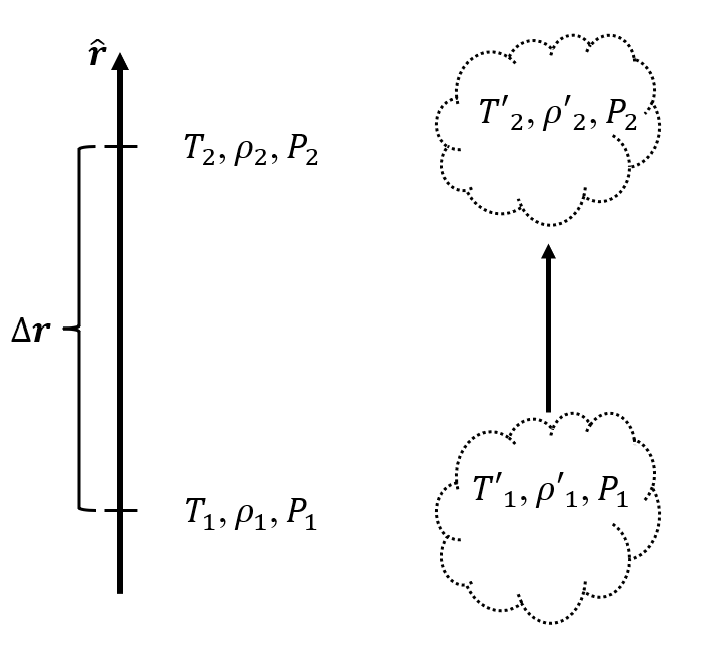
\includegraphics[width=0.5\linewidth]{Appendices//Convec Transport/convection.png}
    \caption{Two points of interest are considered within a plane parallel region of a star. The gas in the surroundings of the star has temperature $T$, density $\rho$, and pressure $P$, while quantities within the gas parcel are primed. Note that $P' = P$ since the gas parcel is assumed to have the same pressure as its surroundings. During convective motion, the gas parcel rise from position 1 to position 2 adiabatically, then dissolves. The distance between position 1 and position 2, $\Delta r$, is of order the mixing length.}
    \label{fig:convec_diagram}
\end{figure}

Suppose that the temperature within the gas parcel is greater than that of the surroundings: $T' > T$. Since pressures are balanced, $\rho' < \rho$. Archimedes' principle states that the parcel experiences a net upwards force

\begin{equation}
    F_\mathrm{buoyancy} = \rho V g - \rho' V g
\end{equation}
%
where  $V$ is the parcel's volume and $g$ is the local gravitational acceleration. Ideally, the parcel starts to rise adiabatically. This strict condition is not realistic, see Chapter 5.1.2 in Ref.~\cite{HK_book} for radiative leakage from convective parcels. The next step depends on the conditions inside the star. The parcel may either continue to rise and eventually dissolve into its new surroundings, or may drop back down. The former outcome is known as convective instability, with the latter indicative of conditions that are stable to convective motion.

\subsection{Convective Stability} \label{ap:convec_stability}
Reviewing assumption (2) in the previous section, the mixing length over which a gas parcel may rise is much smaller than the scale heights within stellar interiors. The pressure scale height given by

\begin{equation}
    \lambda_P = - \frac{P}{dP/dr} = - \bigparenthesis{\pderiv{\ln P}{r}}^{-1} = \frac{P}{g\rho}
\end{equation}

which encapsulates the e-folding distance over which the density changes appreciably. Since $\ell << \lambda_P$, we may assume that the acceleration due to gravity $g$ also does not change appreciably over the mixing length. As such, for a parcel of gas to cease experiencing a net buoyant force upwards, the following condition must be satisfied:

\begin{equation}
    \bigparenthesis{\pderiv{\rho}{r}}_\mathrm{parcel} > \bigparenthesis{\pderiv{\rho}{r}}_\mathrm{star}
\end{equation}
%
Note that $\partial \rho / \partial r$ is a negative quantity. The goal is to express the above condition in terms of local properties. I begin from the differential density, which has dependencies on temperature and pressure via the ideal gas equation of state:

\begin{equation}
    d\rho = \bigparenthesis{\pderiv{\rho}{P}}dP + \bigparenthesis{\pderiv{\rho}{T}} dT
\end{equation}
%
In order to rewrite the various terms in the above equation in terms of thermodynamic quantities, one can divide both sides by $\rho$ and multiply each term by the corresponding quantity:

\begin{align}
    \frac{d\rho}{\rho} &= \frac{1}{\rho} \frac{P}{P}\pderiv{\rho}{P} dP + \frac{1}{\rho}\frac{T}{T} \pderiv{\rho}{T} dT \\
    &= \frac{P}{\rho} \pderiv{\rho}{P}\frac{dP}{P} + \frac{T}{P}\pderiv{\rho}{T}\frac{dT}{T} \\
    &= \alpha \frac{dP}{P} - \delta \frac{dT}{T}
\end{align}
%
As such, the density gradient can be obtained by dividing by the differential $dr$:

\begin{equation}
    \frac{1}{\rho} \pderiv{\rho}{r} = \frac{\alpha}{P} \pderiv{P}{r} - \frac{\delta}{T} \pderiv{T}{r}
\end{equation}
%
The condition for convective stability now reads

\begin{equation}
    \bigparenthesis{\frac{\alpha}{P} \pderiv{P}{r} - \frac{\delta}{T} \pderiv{T}{r}}_\mathrm{parcel} > \bigparenthesis{\frac{\alpha}{P} \pderiv{P}{r} - \frac{\delta}{T} \pderiv{T}{r}}_\mathrm{star}
\end{equation}
%
since pressure in the gas parcel is in balance with the surrounding gas, the first term on each side drops out.

\begin{equation}
    \bigparenthesis{\frac{\delta}{T} \pderiv{T}{r}}_\mathrm{parcel} < \bigparenthesis{\frac{\delta}{T} \pderiv{T}{r}}_\mathrm{star}
\end{equation}
%
Rewriting this condition in terms of logarithmic derivatives, we can multiply by the pressure scale height and cancel $\delta$:

\begin{align}
    \bigparenthesis{-\frac{P}{dP/dr} \frac{1}{T} \pderiv{T}{r}}_\mathrm{parcel} &> \bigparenthesis{-\frac{P}{dP/dr}\frac{1}{T} \pderiv{T}{r}}_\mathrm{star} \\
    \bigparenthesis{\pderiv{\ln T}{\ln P}}_\mathrm{parcel} &> \bigparenthesis{\pderiv{\ln T}{\ln P}}_\mathrm{star}
\end{align}
%
The left-hand-side is merely the adiabatic temperature gradient $\nabla_\mathrm{ad}$, while the right-hand-side requires explanation. This quantity is, in theory, also a temperature gradient. In the absence of convection, radiative diffusion is the mechanism via which energy is transported. Since we seek a condition wherein convection sets in, we assume that radiative transport is happening by default, and label the right-hand-side as $\nabla_\mathrm{rad}$. Finally, we arrive at the Schwarzschild stability criterion:

\begin{empheq}[box=\fbox]{equation}
    \nabla_\mathrm{rad} < \nabla_\mathrm{ad}
\end{empheq}
%
That is, convection kicks in once the radiative temperature gradient exceeds its adiabatic counterpart. If one relaxes the assumption of chemical homogeneity and uniform ionization, the Ledoux stability criterion applies,

\begin{equation}
 \nabla_\mathrm{rad} - \frac{\varphi}{\delta}\bigparenthesis{\pderiv{\ln\mu}{\ln P}} < \nabla_\mathrm{ad},    
\end{equation}
%
where $\varphi = \bigparenthesis{\pderiv{\ln \rho}{\ln \mu}}_{\mathrm{P,T}}$ is the chemical potential and $\mu$ is the mean molecular weight.

\subsection{Energy Transport via Convection}
I now end with the transport of energy by convection. The temperature change in the ambient stellar gas resulting from heat deposited by the parcel is given by

\begin{equation}
    \Delta T = \left[\bigparenthesis{\pderiv{T}{r}}_\mathrm{star} - \bigparenthesis{\pderiv{T}{r}}_\mathrm{parcel} \right] \ell.
\end{equation}
%
We also know that the temperature gradient is given by

\begin{equation}
    \pderiv{T}{r} = \frac{T}{P} \bigparenthesis{\pderiv{\ln T}{\ln P}} \pderiv{P}{r},
\end{equation}
%
giving

\begin{equation}
    \Delta T = \left[ \bigparenthesis{\pderiv{\ln T}{\ln P}}_\mathrm{star} - \bigparenthesis{\pderiv{\ln T}{\ln P}}_\mathrm{parcel} \right] \frac{T}{P} \pderiv{P}{r} \ell.
\end{equation}
%
Replacing the corresponding quantities in the above Equation with $\nabla$s and the pressure scale height, we obtain

\begin{equation}
    \frac{\Delta T}{T} = -\left(\nabla_\mathrm{rad} - \nabla_\mathrm{ad}\right) \omega
\end{equation}
%
where $\omega = \ell/\lambda_P$, the ratio between the mixing length and the pressure scale height creatively labeled the ``mixing length parameter". We can now define the rate of heat transport by convection across a fiducial surface as

\begin{equation}
    \Phi_\mathrm{conv} = \rho c_P \Delta T v_\mathrm{parcel}
\end{equation}
%
where $c_P$ is the specific heat at constant pressure, $\rho$ is the density of the gas parcel, and $v_\mathrm{parcel}$ is the typical speed of a rising parcel. All that remains is to determine this speed. The local buoyant acceleration of the parcel may be written as

\begin{equation}
    g' = g\left|\frac{\Delta \rho}{\rho}\right|,
\end{equation}
%
which, via conservation of energy (per unit mass), relates

\begin{align}
    v_\mathrm{parcel}^2 &= g' \ell \\
    v_\mathrm{parcel} &= \sqrt{g\left|\frac{\Delta \rho}{\rho}\right|\ell} \\
    v_\mathrm{parcel} &= \sqrt{\omega \frac{P}{\rho} \left|\frac{\Delta T}{T}\right|}
\end{align}
%
where the final equality follows from the ideal gas equation of state and the definition of the mixing length parameter $\omega$. Combining everything, we arrive at the expression for convective flux:

\begin{empheq}[box=\fbox]{equation}
\Phi_\mathrm{conv} = \omega^2 \rho c_P T \sqrt{\frac{P}{\rho}} \left(\nabla_\mathrm{rad} - \nabla_\mathrm{ad} \right)^{3/2}
\end{empheq}
%
The quantity in parentheses must be positive for convective motion. The parameter $\omega$ is free and tweaked according to stellar models. When evaluating energy transport in stellar model codes, the following heuristic~\cite{EracleousPSU} is used:
\begin{enumerate}
    \item Assume radiative diffusion is the default mode of energy transport.
    \item Calculate the stellar model.
    \item Check the convective stability throughout the model.
    \begin{enumerate}
        \item For regions that are stable, do nothing.
        \item For regions that are unstable, replace $\Phi_\mathrm{rad}$ with $\Phi_\mathrm{conv}$ and recalculate the model.
    \end{enumerate}
\end{enumerate}

\end{document}
